%-------------------------------PPT Title-------------------------------------
\title{分子动力学概要}
%----------------------------Author & Date------------------------------------

%\author[\textrm{Jun\_Jiang}]{姜\;\;骏\inst{}} %[]{} (optional, use only with lots of authors)
%% - Give the names in the same order as the appear in the paper.
%% - Use the \inst{?} command only if the authors have different
%%   affiliation.
\institute[BCC]{\inst{}%
%\institute[Gain~Strong]{\inst{}%
\vskip -20pt 北京市计算中心~云平台事业部}
%\vskip -20pt {\large 格致斯创~科技}}
\date[\today] % (optional, should be abbreviation of conference name)
{%	{\fontsize{6.2pt}{4.2pt}\selectfont{\textcolor{blue}{E-mail:~}\url{jiangjun@bcc.ac.cn}}}
\vskip 45 pt {\fontsize{8.2pt}{6.2pt}\selectfont{%清华大学\;\;物理系% 报告地点
	\vskip 5 pt \textrm{2023.11}}}
}

%% - Either use conference name or its abbreviation
%% - Not really information to the audience, more for people (including
%%   yourself) who are reading the slides onlin%%   yourself) who are reading the slides onlin%%   yourself) who are reading the slides onlineee
%%%%%%%%%%%%%%%%%%%%%%%%%%%%%%%%%%%%%%%%%%%%%%%%%%%%%%%%%%%%%%%%%%%%%%%%%%%%%%%%%%%%%%%%%%%%%%%%%%%%%%%%%%%%%%%%%%%%%

\subject{}
% This is only inserted into the PDF information catalog. Can be left
% out.
%\maketitle
\frame
{
%	\frametitle{\fontsize{9.5pt}{5.2pt}\selectfont{\textcolor{orange}{“高通量并发式材料计算算法与软件”年度检查}}}
\titlepage
}
%-----------------------------------------------------------------------------

%------------------------------------------------------------------------------列出全文 outline ---------------------------------------------------------------------------------
\section*{}
\frame[allowframebreaks]
{
  \frametitle{Outline}
%  \frametitle{\textcolor{mycolor}{\secname}}
  \tableofcontents%[current,currentsection,currentsubsection]
}
%%在每个section之前列出全部Outline
%%类似的在每个subsection之前列出全部Outline是\AtBeginSubsection[]
%\AtBeginSection[]
%{
%  \frame<handout:0>%[allowframebreaks]
%  {
%    \frametitle{Outline}
%%全部Outline中,本部分加亮
%    \tableofcontents[current,currentsection]
%  }
%}

%-----------------------------------------------PPT main Body------------------------------------------------------------------------------------
\small
\section{晶格振动与分子动力学}
\frame
{
	\frametitle{原子间相互作用力的表示}
	\textcolor{blue}{质点运动发生在一个几何空间里,所以力学可以看成是某个几何空间里的动力系统}。正因此,力学常被冠以``动力学''的称呼
\vskip 1pt
	分子动力学模拟中最主要因素是\textcolor{purple}{原子间相互作用力}
\begin{itemize}
	\item 经典分子动力学模拟中,原子间相互作用力是根据经验势函数得到的\footnote{\fontsize{6.2pt}{4.2pt}\selectfont{经验势函数也称为力场,是参数化形式给出的原子间相互作用,一般通过对实验数据拟合或小体系的第一原理计算得到}}。构建一套高精度的经验势函数代价很高,而且经验势函数一般不具备可移植性
\end{itemize}
\vskip 5pt
	当动力学过程必须考虑量子效应(如电子影响的贡献不可忽略时),必须采用第一原理分子动力学\textrm{(Ab initio~MD,~AIMD)}
	\begin{itemize}
		\item 所谓第一原理分子动力学,就是在计算原子运动时,将电子结构变化的贡献考虑进来,因此在每一时间步长,体系实时构型下的原子受力计算,都必须伴随电子结构计算
	\end{itemize}
	一般电子结构计算采用\textrm{DFT}计算,不难想见,第一原理分子动力学模拟的代价极高
}

\subsection{晶格振动与简谐振动}
\frame
{
	\frametitle{晶格振动}
		晶体中的格点表示原子的平衡位置,晶格振动是原子在格点附近的振动
\begin{figure}[h!]
\centering
%\hspace*{-10pt}
\vspace*{-0.1in}
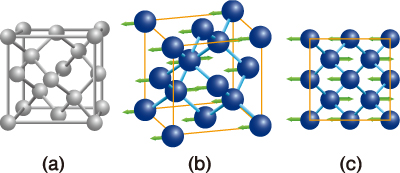
\includegraphics[height=1.9in,width=4.0in,viewport=0 0 400 185,clip]{Figures/Schematic-diagrams-of-the-crystal-structures-and-longitudinal-optical-lattice-vibration-modes-(LO_modes)-of-diamonds.jpg}
\caption{\tiny \textrm{Schematic diagrams of the crystal structures and longitudinal optical lattice vibration modes (LO modes) of diamonds. (a) Crystal structure of a diamond. (b) 3D view of a LO mode. (c) Top view of a LO mode.}}%
\label{lattice-virbration}
\end{figure} 
}

\frame
{
	\frametitle{简谐近似}
	\begin{itemize}
		\item 红外、\textrm{Raman}光谱、中子衍射谱,热容、热导,电阻、超导和电-声耦合等都与晶格振动有关
		\item 绝热近似%(\textrm{Born-Oppenheimer}近似)
			下,原子核是在电子能量函数$E(\mathbf{R})$构成的势能面上运动
	\end{itemize}
	含有$N$个原子,平衡位置是$\mathbf{R}_i^0$,偏移位置矢量$\mathbf{\mu}_i(t)$,体系的势能函数在平衡位置作\textrm{Taylor~}级数展开
	\begin{displaymath}
%		\begin{aligned}
		V=V_0+\sum_{i=1}^{3N}\left( \frac{\partial V}{\partial \mu_i} \right)_0\mu_i+\underline{\textcolor{red}{\frac12\sum_{i,j=1}^{3N}\left( \frac{\partial^2V}{\partial\mu_i\partial\mu_j} \right)_0\mu_i\mu_j}}+\mbox{高阶项}
%		\end{aligned}
	\end{displaymath}
	平衡位置$\left( \frac{\partial V}{\partial\mu_i} \right)_0=0$\\
	\textcolor{blue}{简谐近似}保留到$\mu_i$的二次项\\
	引入高阶项,则势函数可以包括\textcolor{purple}{非简谐近似}的贡献
}

\frame
{
	\frametitle{简谐振动与简正坐标}
	$N$原子体系的动能函数
	\begin{displaymath}
		T=\frac12\sum_{i=1}^{3N}m_i\dot{\mu}_i^2
	\end{displaymath}
	引入简正坐标,\textcolor{blue}{与原子位移坐标$\mu_i$正交变换}
	\begin{displaymath}
		\sqrt{m_i}\mu_i=\sum_{j=1}^{3N}a_{ij}Q_j
	\end{displaymath}
	\textcolor{red}{目的}:~系统的势能函数与动能函数有简单形式(只有平方项)
	\begin{displaymath}
%		\begin{aligned}
			T=\frac12\sum_{i=1}^{3N}\dot{Q}_i^2\quad
			V=\frac12\sum_{i=1}^{3N}\omega_i^2Q_i^2
%		\end{aligned}
	\end{displaymath}
	由此可得谐振方程
	\begin{displaymath}
		\ddot{Q}_i+\omega_i^2Q_i=0\quad i=1,2,3,\cdots,3N
	\end{displaymath}

}

\frame
{
	\frametitle{简谐振动与振动模式}
	任意简正坐标解
	\begin{displaymath}
		Q_i=A\sin(\omega_it+\delta)
	\end{displaymath}
	由此得到原子位移坐标
	\begin{displaymath}
		\mu_i=\frac{a_{ij}}{\sqrt{m_i}}A\sin(\omega_it+\delta)
	\end{displaymath}
\begin{figure}[h!]
\centering
%\hspace*{-10pt}
\vspace*{-0.1in}
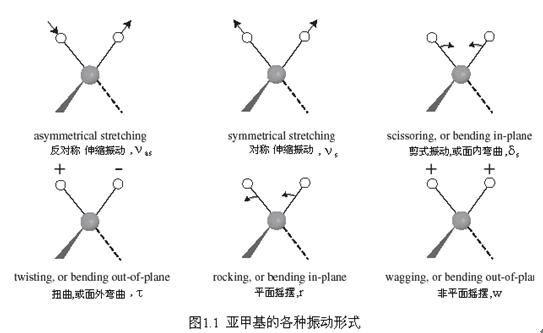
\includegraphics[height=1.in,width=2.in,viewport=0 20 420 250,clip]{Figures/RF_vir.jpg}
\caption{\tiny \textrm{Schematic example of vibration model of dimethyl.}}%
\label{virbration_model}
\end{figure} 
\textcolor{red}{简谐振动不表示某个原子的振动,表示整个体系所有原子参与的振动。这种体系中所有原子一起参加的集体运动常称为振动模}
}

\frame
{
	\frametitle{简谐振动与振动模式}
\begin{figure}[h!]
\centering
%\hspace*{-10pt}
\vspace*{-0.05in}
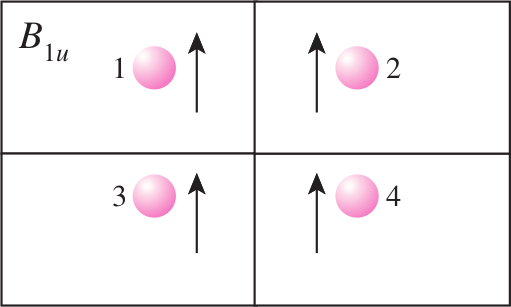
\includegraphics[height=1.1in,width=1.95in,viewport=0 0 520 310,clip]{Figures/Viberation_of_B1u.png}
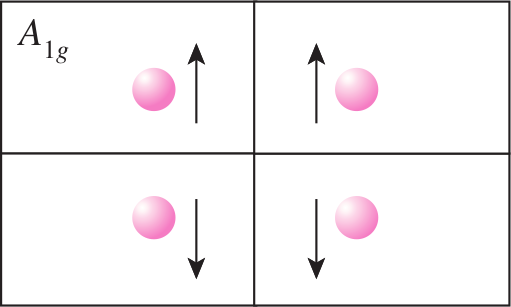
\includegraphics[height=1.1in,width=1.95in,viewport=0 0 515 310,clip]{Figures/Viberation_of_A1g.png}
\vskip 4pt
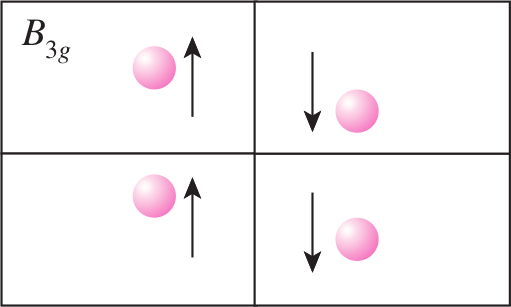
\includegraphics[height=1.1in,width=1.95in,viewport=0 0 520 310,clip]{Figures/Viberation_of_B3g.png}
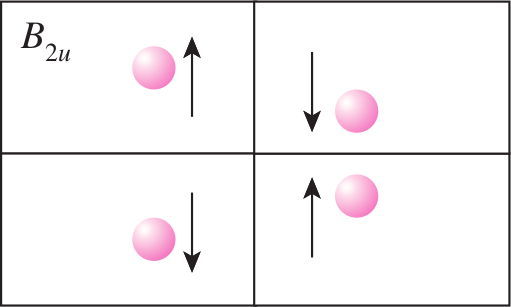
\includegraphics[height=1.1in,width=1.95in,viewport=0 0 515 310,clip]{Figures/Viberation_of_B2u.png}
\caption{\tiny \textrm{Schematic example of the symmetry of vibration model.}}%
\label{virbration_model-symmetry}
\end{figure} 
}

\frame
{
	\frametitle{一维单原子链}
\begin{figure}[h!]
\centering
%\hspace*{-10pt}
\vspace*{-0.25in}
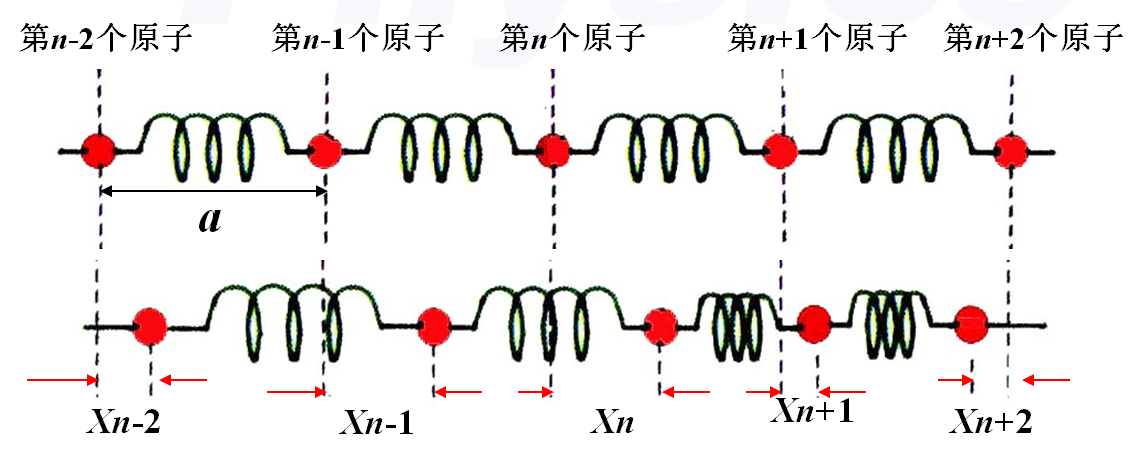
\includegraphics[height=1.0in,width=2.8in,viewport=0 0 1400 500,clip]{Figures/virbration.png}
\caption{\tiny \textrm{Schematic example of vibration of 1D-atomic chain.}}%
\label{virbration}
\end{figure} 
单原子链可以视为最简单的晶格,平衡时相邻原子距离为$\mathbf{a}$,原子限制在沿链方向运动,偏离格点位置用$\cdots,\mathbf{X}_{n-1},\mathbf{X}_{n},\mathbf{X}_{n+1},\cdots$,原子的振动可以表示为
\begin{displaymath}
	\mu_{nq}=A\mathrm{e}^{\mathrm{i}(\omega t-qx)}
\end{displaymath}
其中振幅$A$是常数,$\omega$是圆频率,$q=\tfrac{2\pi}{\lambda}$是波数,$\lambda$是波长
\vskip 5pt
\textcolor{blue}{根据量子理论,每种简谐振动的能量是量子化的,可以用声子表示}
\begin{displaymath}
	\varepsilon_{nq}=\left( n+\frac12 \right)\hbar\omega_q
\end{displaymath}
}

\frame
{
	\frametitle{谐振子模型}
\begin{figure}[h!]
\centering
%\hspace*{-10pt}
\vspace*{-0.15in}
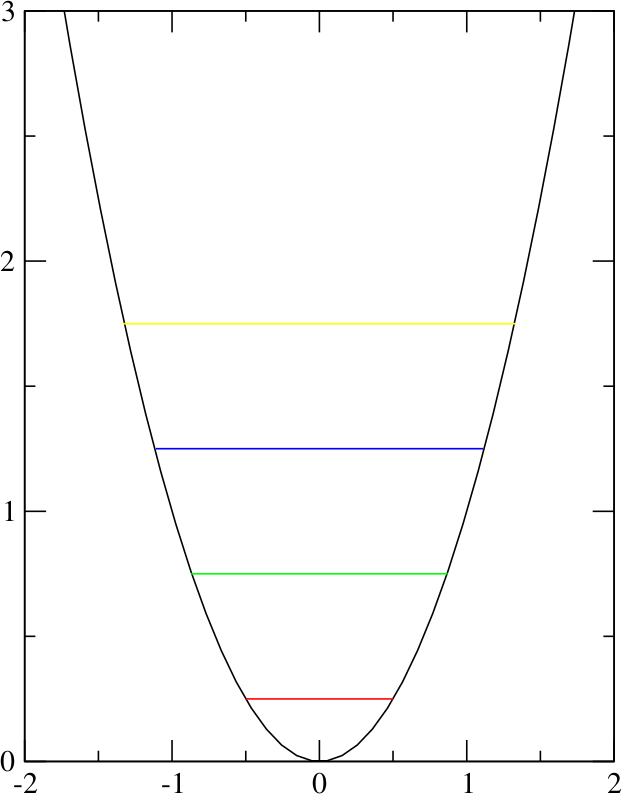
\includegraphics[height=2.7in,width=2.9in,viewport=0 0 650 800,clip]{Figures/Quantum-viberation.png}
\caption{\tiny \textrm{Schematic example of quantization of  harmonic oscillator model.}}%
\label{Harmonic-oscillator-model}
\end{figure} 
}

\frame
{
	\frametitle{双原子链与光学支和声学支}
\begin{figure}[h!]
\centering
%\hspace*{-10pt}
\vspace*{-0.20in}
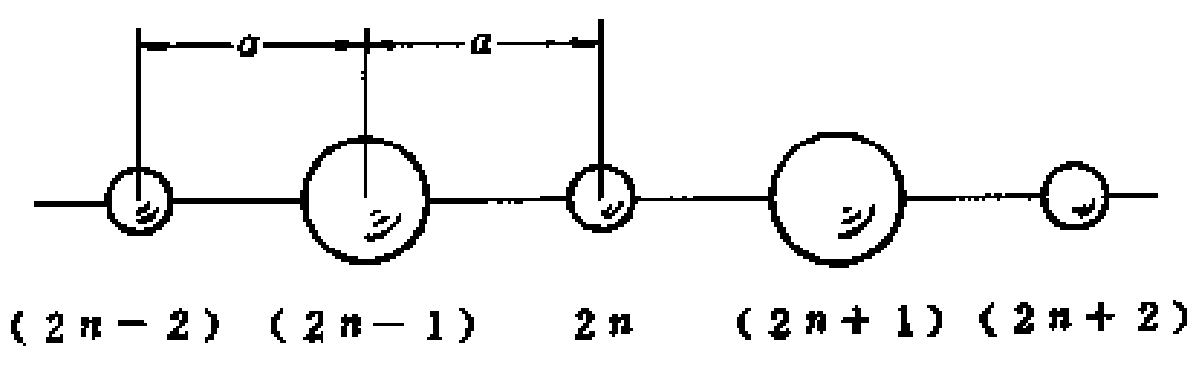
\includegraphics[height=0.7in,width=2.6in,viewport=0 0 1400 400,clip]{Figures/virbration-2.png}
\caption{\tiny \textrm{Schematic example of vibration of 1D-diatomic chain.}}%
\label{virbration-2D}
\end{figure} 
一维双原子链是最简单的复式晶格,平衡时相邻原子间距为$\mathbf{a}$,每个原胞含有两个不同原子\textrm{P}和\textrm{Q},质量分别是$m$和$M$,原子现在在沿链方向运动,偏离位移用$\cdots,\mu_{2n},\mu_{2n+1},\cdots$\\原子的运动方程
\begin{displaymath}
	\begin{aligned}
		&\mbox{\textrm{P}原子:~}m\ddot{\mu}_{2n}=-\beta(2\mu_{2n}-\mu_{2n+1}-\mu_{2n-1})\\
		&\mbox{\textrm{Q}原子:~}M\ddot{\mu}_{2n+1}=-\beta(2\mu_{2n+1}-\mu_{2n+2}-\mu_{2n})
	\end{aligned}
\end{displaymath}
可得关于振动频率$\omega$的两组解
\begin{displaymath}
	\omega^2\left.
	\begin{aligned}
		&\nearrow\omega_+^2\\
		&\searrow\omega_-^2
	\end{aligned}\right\}
	=\beta\frac{m+M}{mM}\left\{ 1\pm\left[ 1-\frac{4mM}{(m+M)^2}\sin^2aq \right]^{1/2} \right\}
\end{displaymath}
}

\frame
{
	\frametitle{光学支和声学支的长波极限}
\begin{figure}[h!]
\begin{minipage}[t]{0.3\linewidth}
\centering
\vspace*{-0.3in}
%\hspace*{-10pt}
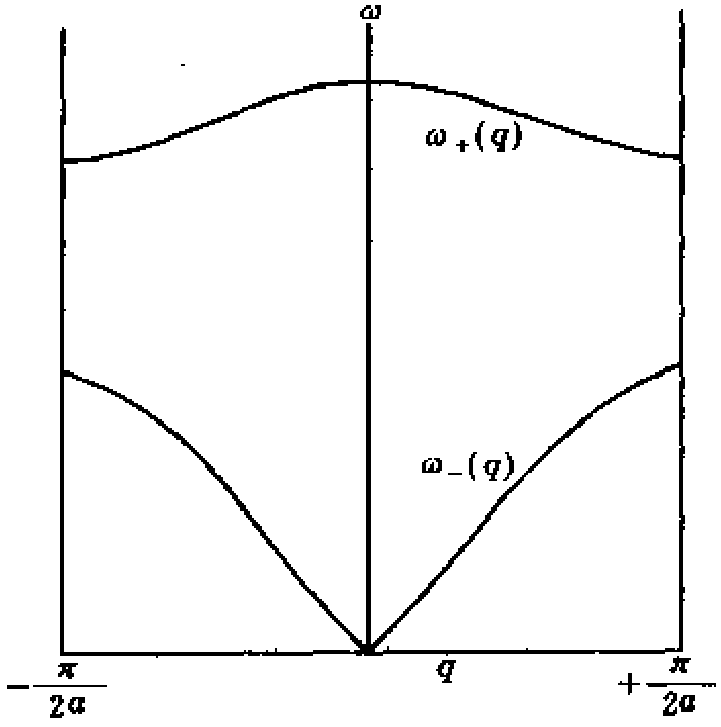
\includegraphics[height=1.in,width=1.in,viewport=0 0 700 800,clip]{Figures/Optic-Acous.png}
\label{optic_acous}
\end{minipage}
\hfill
\begin{minipage}[t]{0.67\linewidth}
%\vspace*{-0.3in}
	\begin{itemize}
		\item \textcolor{blue}{光学支}:~属于频率$\omega_+$的晶格简谐振动
		\item \textcolor{blue}{声学支}:~属于频率$\omega_-$的晶格简谐振动
	\end{itemize}
\end{minipage}
\caption{\tiny \textrm{The acoustic branch and optical branch.}}%
\end{figure} 
声学支的长波极限($q\rightarrow0$):
\begin{displaymath}
	\omega_-\approx a\sqrt{\frac{2\beta}{m+M}}q\quad\mbox{\textcolor{blue}{一维链看成连续介质的弹性波}}
\end{displaymath}
光学支的长波极限($q\rightarrow0$):
\begin{displaymath}
	\omega_+\approx a\sqrt{\frac{2\beta}{\left( \frac{mM}{m+M} \right)}}\quad\mbox{\textcolor{blue}{两种原子具有相反的相位,质心保持不动}}
\end{displaymath}
}

\frame
{
	\frametitle{声子振动模式的横向传播与纵向传播}
\begin{figure}[h!]
\centering
%\hspace*{-10pt}
\vspace*{-0.30in}
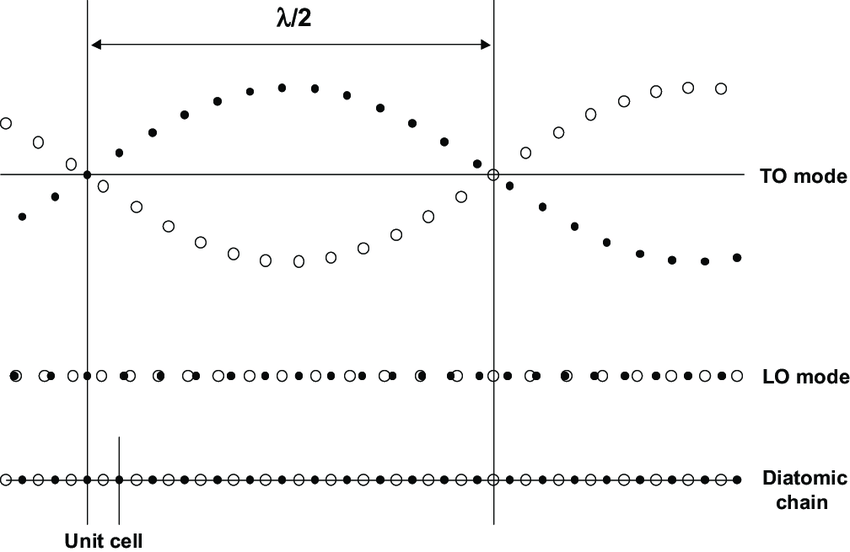
\includegraphics[height=2.5in,width=4.0in,viewport=0 0 850 610,clip]{Figures/examples-of-transverse-optical-to-and-longitudinal-optical-lo-phonons-in-1d.png}
\caption{\tiny \textrm{Schematic examples of transverse optical to and longitudinal optical phonons in 1d diatomic lattice.}}%
\label{To-Lo-1D}
\end{figure} 
}

\frame
{
	\frametitle{声学支和光学支的长波极限}
\begin{figure}[h!]
\centering
%\hspace*{-10pt}
\vspace*{-0.10in}
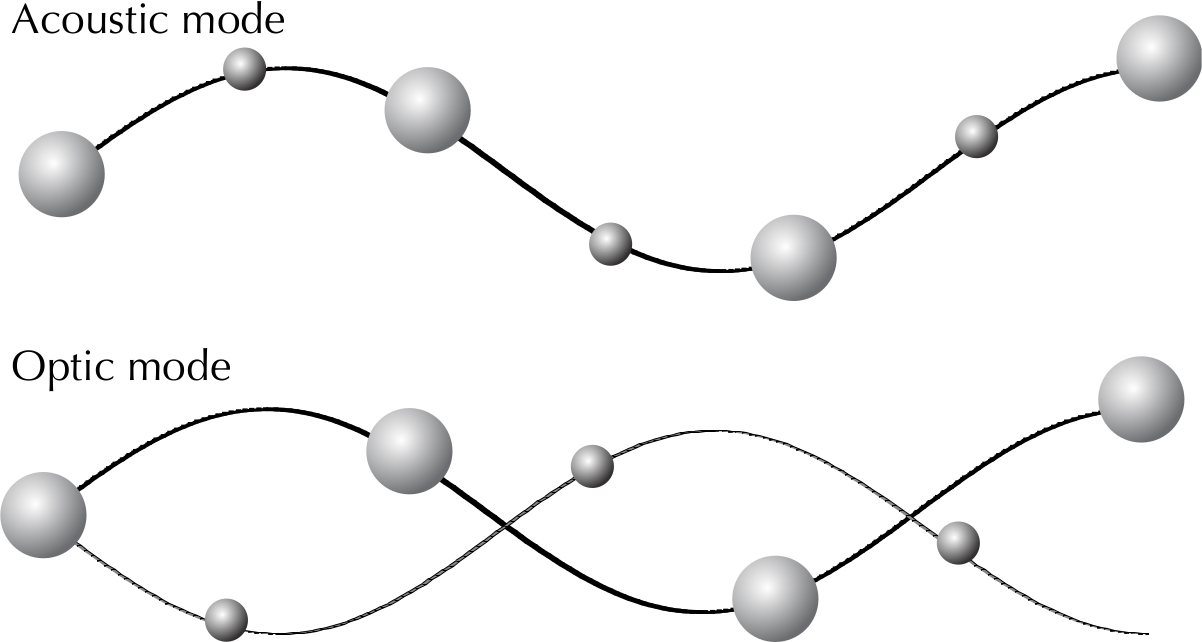
\includegraphics[height=2.3in,width=4.0in,viewport=0 0 1210 650,clip]{Figures/Phonon-Acoutic-Optic.png}
\caption{\tiny \textrm{Representation of the difference between acoustic and optic modes in the limit of wave vector $\vec q\rightarrow0$ for the model diatomic chain: acoustic (in-phase) and optic (out-of-phase) modes.}}%
\label{Aucous-Optic}
\end{figure} 
}

\frame
{
	\frametitle{经典三维振动模式}
	位于$\mathbf{R}_I(t)$的原子核运动的经典力学描述
			\begin{displaymath}
				M_I\frac{\partial^2\mathbf{R}_I}{\partial t^2}=\vec F_I(\mathbf{R})=-\frac{\partial}{\partial\mathbf{R}_I}E(\mathbf{R})
			\end{displaymath}
			晶格平衡位置$\{\mathbf{R}_I^0\}=\mathbf R^0$由原子核受力平衡确定
			\begin{displaymath}
				\vec F_I(\mathbf R^0)=0
			\end{displaymath}
			\textcolor{blue}{对平衡位置偏移的受力方程为}
			\begin{displaymath}
				C_{I,\alpha;J,\beta}=\frac{\partial^2E(\mathbf{R})}{\partial\mathbf{R}_{I,\alpha}\partial\mathbf{R}_{J,\beta}}
			\end{displaymath}
			其中$\alpha,\beta\cdots$是\textrm{cartesian}坐标

			\textcolor{blue}{谐振子近似下},频率为$\omega$的谐振模式下,晶格对平移位置的偏移为
			\begin{displaymath}
				\mathbf{u}_I(t)=\mathbf{R}_I(t)-\mathbf{R}_I^0\equiv\mathbf{u}_I\mathrm{e}^{\mathrm{i}\omega t}
			\end{displaymath}
}

\frame
{
	\frametitle{三维晶格振动模式}
			对位于$I$的原子核(质量为$M_I$),有
			\begin{displaymath}
				-\omega^2M_Iu_{I\alpha}=-\sum_{J\beta}C_{I,\alpha;J\beta}u_{J\beta}
			\end{displaymath}
			因此振动频率$\omega$,由经典谐振方程确定
%			\begin{displaymath}
%				\det\left|\frac1{\sqrt{M_IM_J}}C_{I,\alpha;J\beta}-\omega^2\right|=0
%			\end{displaymath}
%	对于周期性的晶格振动,根据\textrm{Bl\"och~}定理,振动引起的位置偏移
%			\begin{displaymath}
%				\mathbf{u}_s(\vec T_n)\equiv\mathbf{R}_s(\vec T_n)-\mathbf{R}_s^0(\vec T_n)=\mathrm{e}^{\mathrm{i}\vec k\cdot\vec T_n}\mathbf{u}_s(\vec k)
%			\end{displaymath}
%			由此得谐振方程
			\begin{displaymath}
				\det\left|\frac1{\sqrt{M_sM_{s^{\prime}}}}C_{s,\alpha;s^{\prime}\alpha^{\prime}}-\omega_{i\vec k}^2\right|=0
			\end{displaymath}
			这里原子标记$s=1,\cdots,s$,对应的谐振模式$i=1,\cdots,3s$

			每个$\vec k$的约化力常数矩阵可表示为
			\begin{displaymath}
				\begin{aligned}
				C_{s,\alpha;s^{\prime}\alpha^{\prime}}(\vec k)=&\sum_{\vec T_n}\mathrm{e}^{\mathrm{i}\vec k\cdot\vec T_n}\frac{\partial^2 E(\mathbf{R})}{\partial\mathbf{R}_{s,\alpha}(0)\partial\mathbf{R}_{s^{\prime},\alpha^{\prime}}(\vec T_n)}\\
				=&\frac{\partial^2E(\mathbf{R})}{\partial\mathbf{u}_{s,\alpha}(\vec k)\partial\mathbf{u}_{s^{\prime},\alpha^{\prime}}(\vec k)} 
				\end{aligned}
			\end{displaymath}
}

\section{经典分子动力学提要}
\frame
{
	\frametitle{分子动力学\textrm{(MD)}}
	分子动力学\textrm{(Molecular dynamics,~MD)}主要用于各类化学反应、合金与复杂材料状态方程研究,着重关注体系的反应或状态随温度、压力变化规律和动力学性质
\vskip 5pt
\textcolor{blue}{分子动力学模拟的基本框架}
	\begin{itemize}
		\item 结构优化:~根据体系的初始构型\textrm{(initial configuration)},遵从能量最低原理,得到体系基态结构(确定基态时原子的位置)
		\item 原子运动计算:~在一定环境(温度、压力等)条件下,计算各原子的受力,并依据运动方程得到设定时间步长下的原子的运动,进而获得得体系的当前构型
		\item 径迹计算:~在设定的时间范围内,根据原子运动和体系构型的变化,组合成体系随时间演化的径迹\textrm{(the trajectory of time evolution)}
		\item 结果分析:~分析体系的径迹变化规律,得到体系的动力学和热力学性质
	\end{itemize}
}

\subsection{经典分子动力学简介}
\frame
{
	\frametitle{经典分子动力学}
	装有$N$个经典粒子的$L_1\times L_2\times L_3$容器内,假设粒子间只有简单的二体相互作用\footnote{\fontsize{7.2pt}{6.2pt}\selectfont{二体作用是粒子间多体相互作用的简化,只考虑粒子两两间彼此相互作用。}}$\vec F(r)$,力的大小仅与粒子间间距$r$相关
	\begin{displaymath}
		\vec F(R_i)=\sum_{\substack{j=1\\j\neq i}}^N F(|\vec r_i-\vec r_j|)\hat{\vec r}_{ij}
	\end{displaymath}
	{\fontsize{7.2pt}{6.2pt}\selectfont{这里$R$代表全部原子坐标$\vec r_i$,$\hat{\vec r}_{ij}$是表示粒子$i$指向粒子$j$的矢量($\vec r_j-\vec r_i$)的单位矢量}}

	在经典力学框架下,粒子$i$的受力运动方程是:~
	\begin{displaymath}
		\dfrac{\mathrm{d}^2\vec r_i(t)}{\mathrm{d}t^2}=\dfrac{\vec F_i(R)}{m_i}
	\end{displaymath}
	粒子$i$的质量是$m_i$\\
	\textcolor{purple}{经典分子动力学,就是应用数值模拟对大量粒子求解该方程,基于统计力学原理,研究物质的状态和热力学性质}
}

\frame[allowframebreaks]
{
	\frametitle{经典分子动力学力场}
	原子间受力一般用\textcolor{red}{力场}(\textrm{Force Field},也就是“\textcolor{blue}{相互作用势}”)描述,力场的形式有很多种,典型力场的有
	\begin{itemize}
		\item \textrm{Lennard-Jones}对势
	\begin{displaymath}
		U(r)=4\varepsilon\bigg[\bigg(\dfrac{\sigma}{r}\bigg)^{12}-\bigg(\dfrac{\sigma}{r}\bigg)^6\bigg]
	\end{displaymath}
	{\fontsize{7.2pt}{6.2pt}\selectfont{这里$\varepsilon$和$\sigma$是和原子有关的参数
	\textrm{L-J}势能的最低点在$r_{\min}=2^{(1/6)}\sigma\approx1.12\sigma$,$r<r_{\min}$时为排斥力,$r>r_{\min}$时为吸引力
\begin{figure}[h!]
\centering
\vspace*{-0.30in}
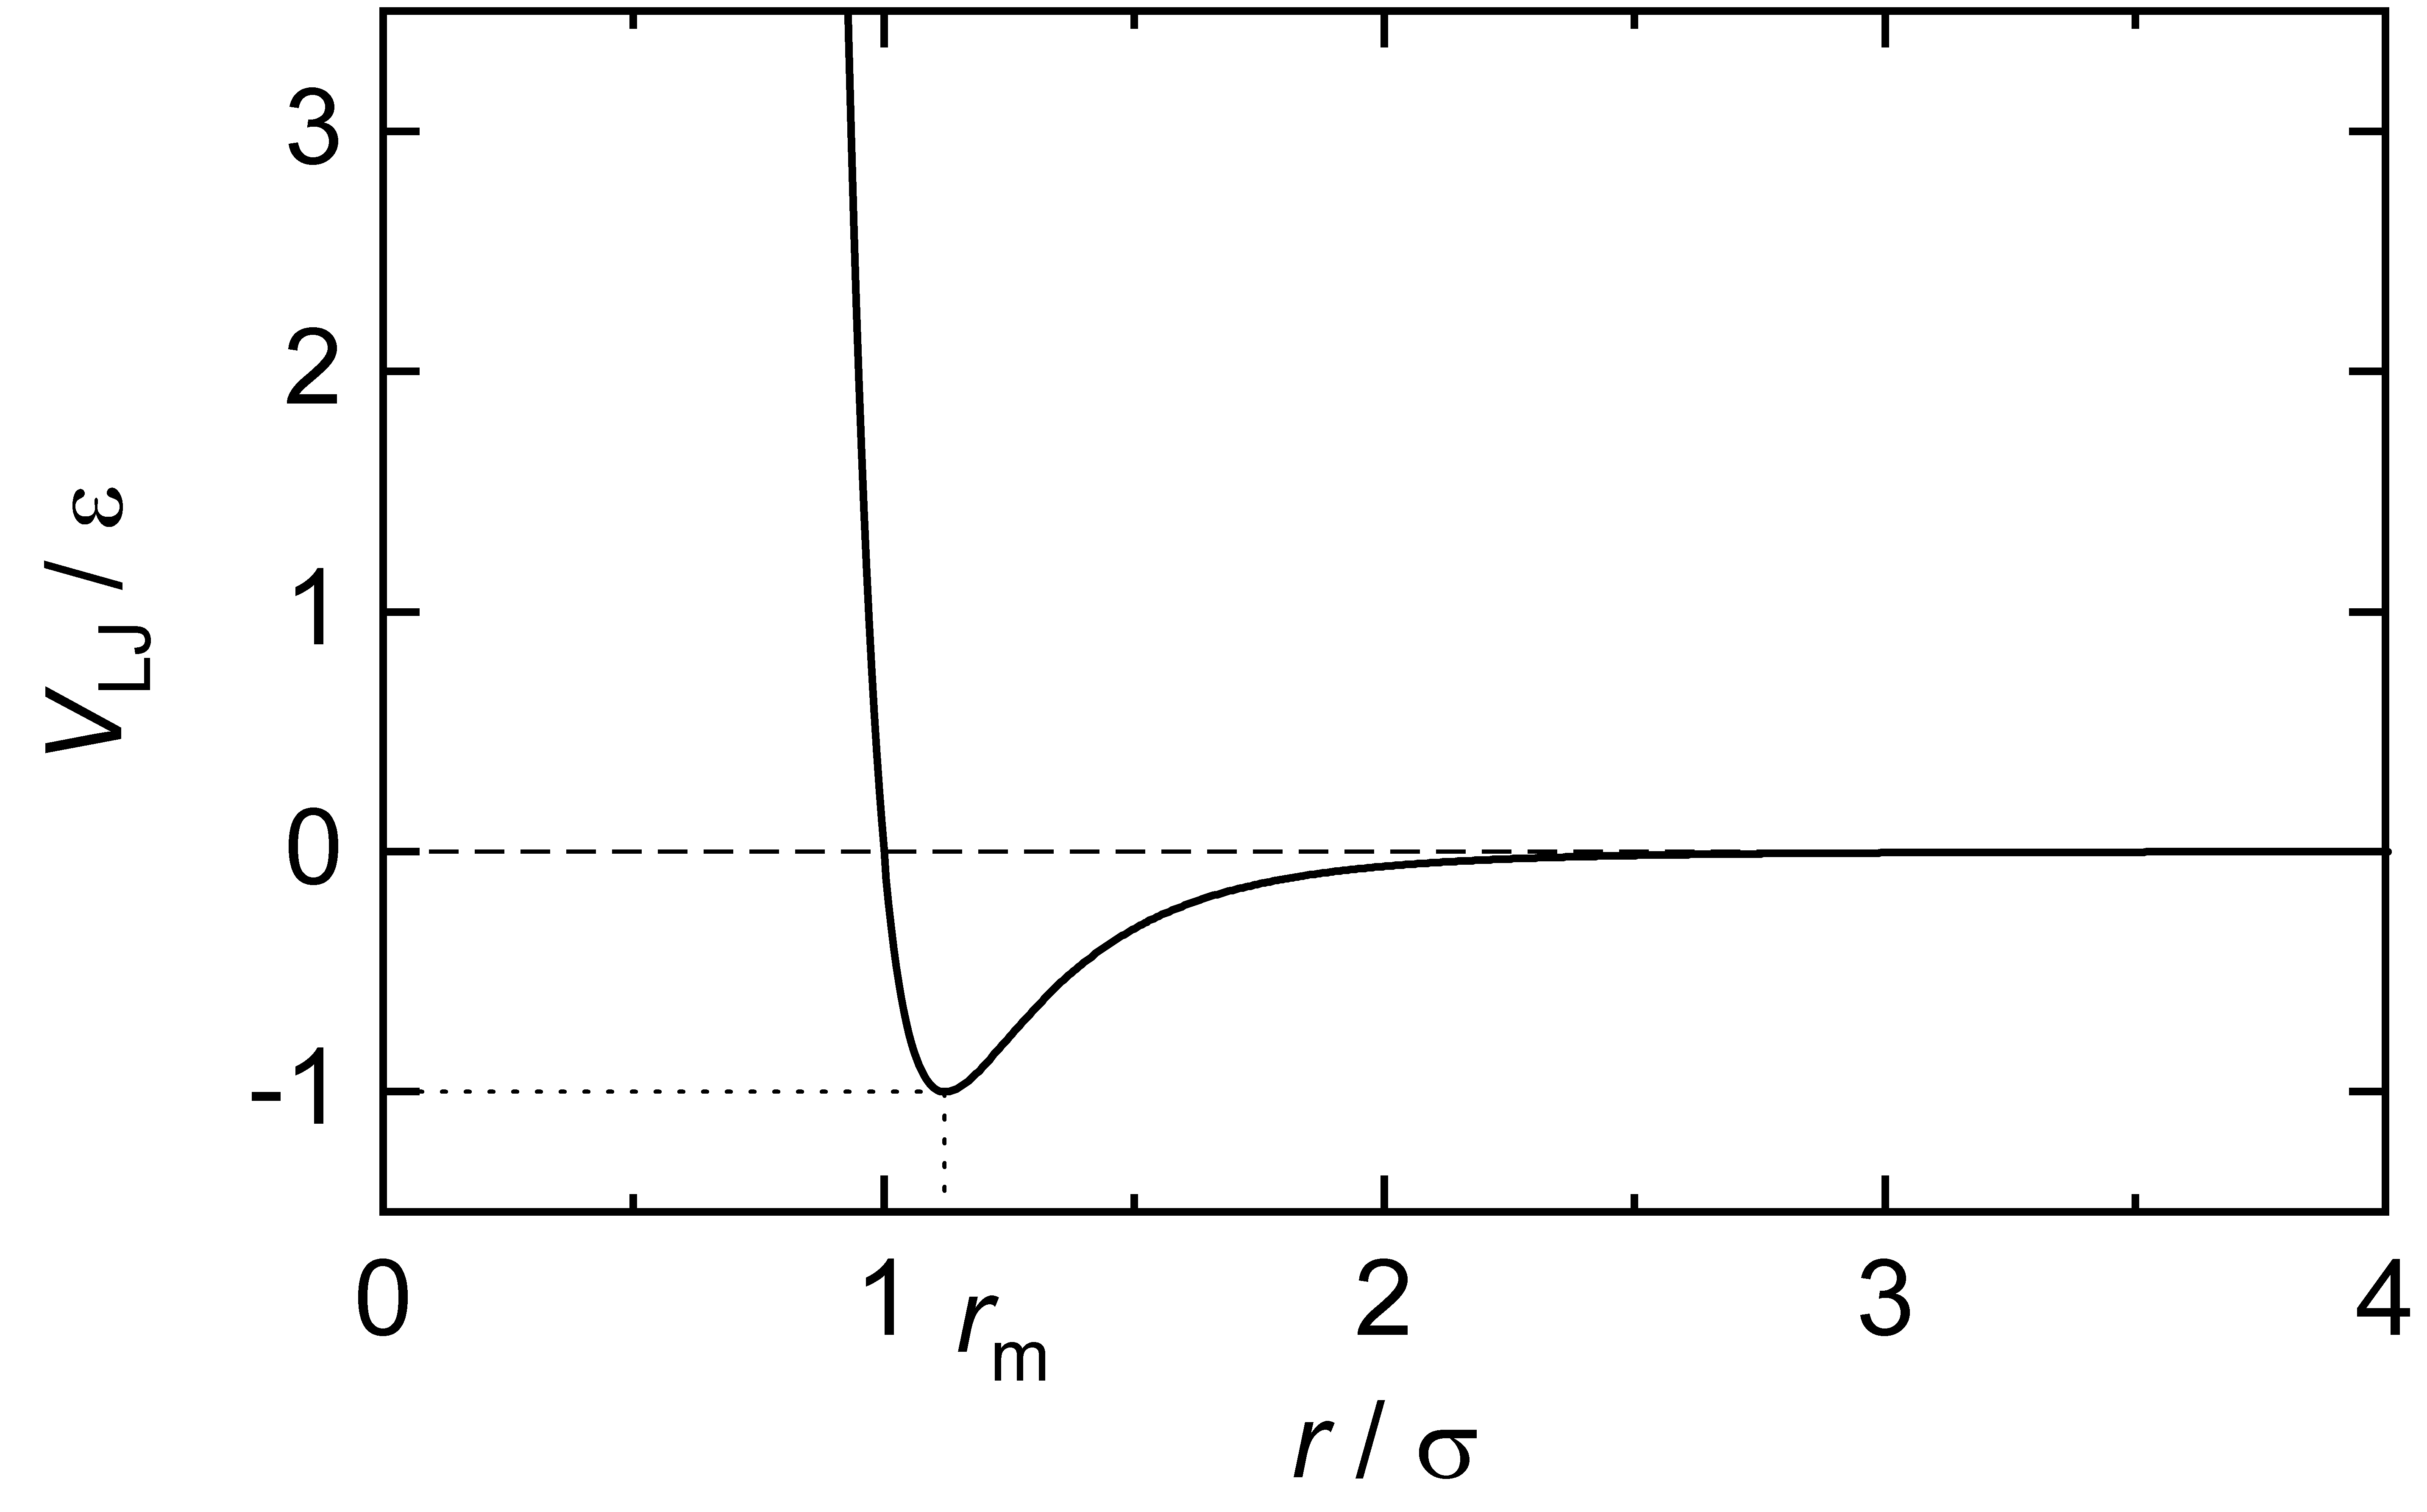
\includegraphics[height=1.00in,width=1.35in,viewport=0 0 340 270,clip]{Figures/Lennard-Jones_potential.png}
\caption{\tiny \textrm{The Lennard-Jones Potential.}}%(与文献\cite{EPJB33-47_2003}图1对比)
\label{Potential-Lennard-Jones}
\end{figure}
\vskip -20pt
	由\textrm{L-J}势改造,可以得到\textrm{WCA}势和\textrm{PHS}势}}
\item \textrm{Morse}势
	\begin{displaymath}
		U(r)=-D_{\mathrm{e}}+D_{\mathrm{e}}\bigg(1-\mathrm{e}^{-a(r-r_{\mathrm{e}})}\bigg)^2
	\end{displaymath}
	{\fontsize{7.2pt}{6.2pt}\selectfont{这里$D_{\mathrm{e}}$是\textrm{Morse}势的势阱深,参数$a$确定势阱宽度,$r_{\mathrm{e}}$是原子处于平衡位置的平衡键长
\begin{figure}[h!]
\centering
\vspace*{-0.15in}
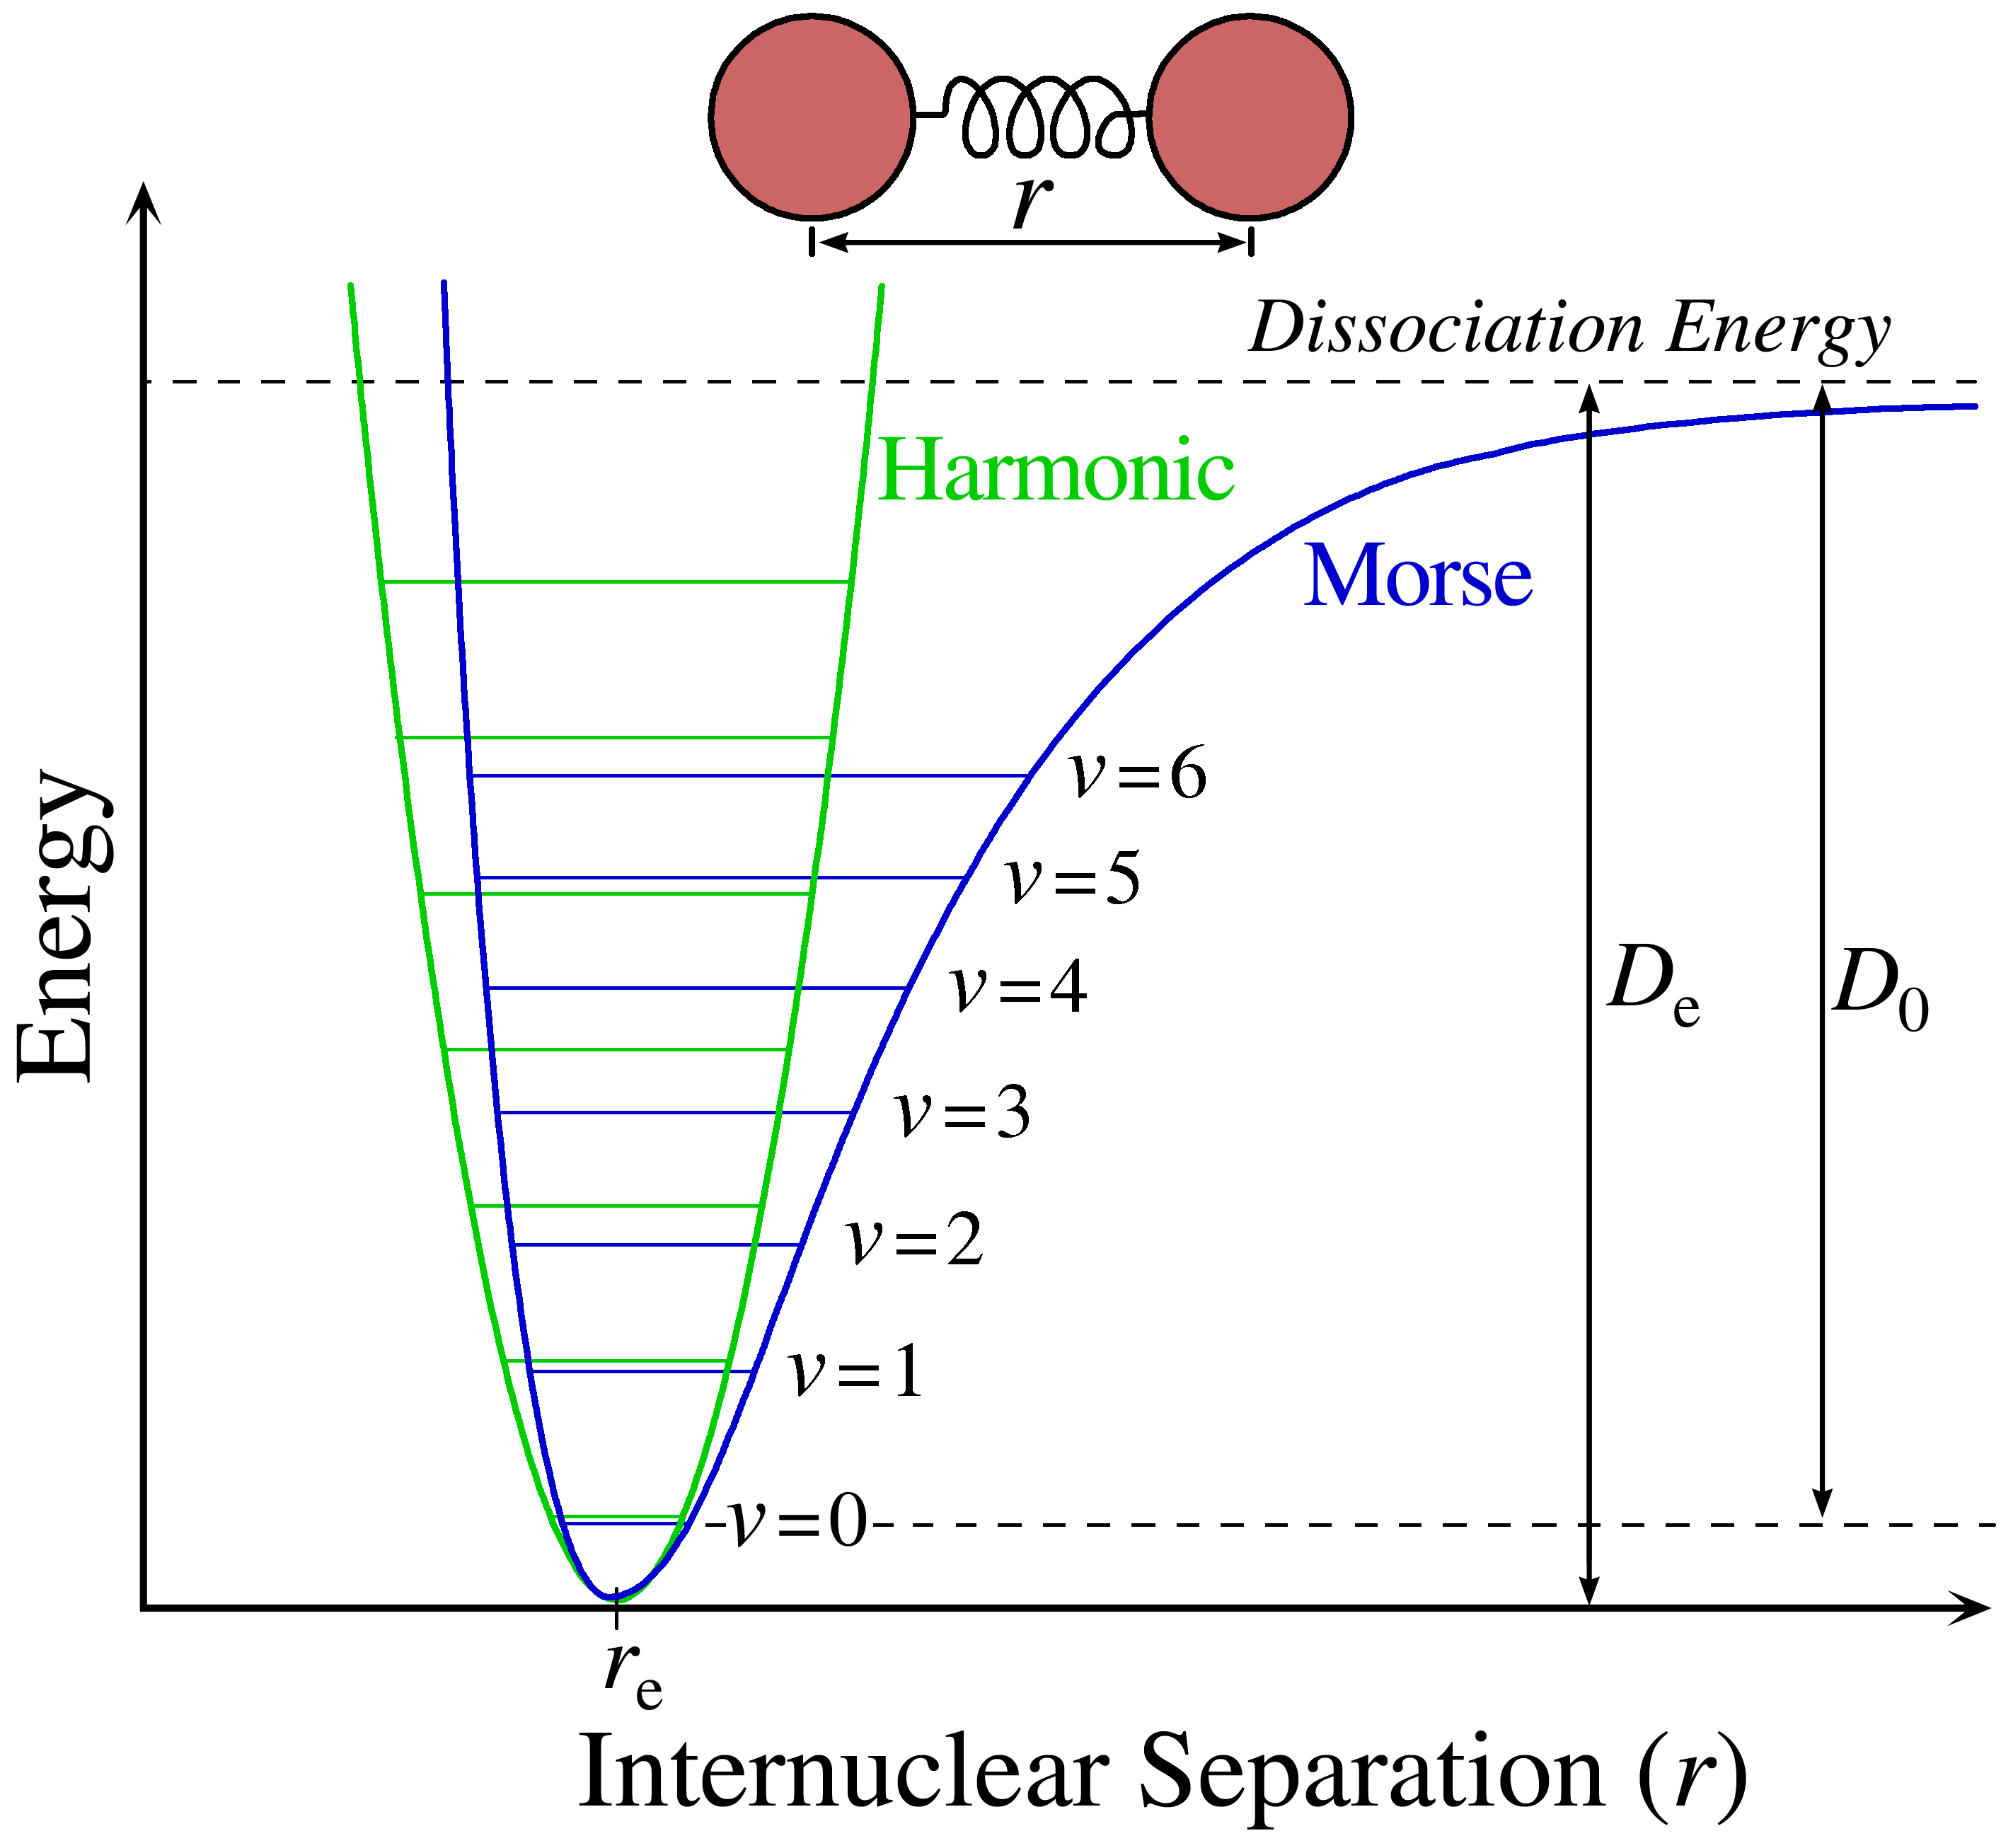
\includegraphics[height=1.30in,width=1.85in,viewport=0 0 3540 2770,clip]{Figures/Morse-potential.png}
\caption{\tiny \textrm{The Morse potential (blue) and harmonic oscillator potential (green).}}%(与文献\cite{EPJB33-47_2003}图1对比)
\label{Potential-Morse}
\end{figure}
}}
\item \textrm{EAM}势\\
	{\fontsize{9.5pt}{6.2pt}\selectfont{对于金属晶体,内能虽可以表示为对相互作用之和,但拟合原子受力非常困难\footnote{\fontsize{5.2pt}{3.2pt}\selectfont{应用二体势计算金属弹性常数时必须涉及对体积很敏感的能量项,因为涉及缺陷、表面的体积很难确定。}}:
	\vskip 2pt
	\textcolor{red}{从物理上说金属原子处于电子海洋中,电子密度来自多个原子的贡献,这是自由电子气带来的多体效应}}
	\vskip 2pt
	\textrm{EAM}将金属中原子的势能表示为二体势和多体势之和
	\begin{displaymath}
		E_i=F_{\alpha}\bigg(\sum_{j\neq i}\rho_{\beta}(r_{ij})\bigg)+\dfrac12\sum_{j\neq i}\phi_{\alpha\beta}(\vec r_{ij})
	\end{displaymath}}
	{\fontsize{7.2pt}{6.2pt}\selectfont{$\alpha$和$\beta$分别为位置$i$、$j$处的原子类型\\
		$\phi$是二体势,是原子$\alpha$和$\beta$和原子间距$r_{ij}$的函数\\
		$F$是多体势,是其余原子在位置$i$处的电荷密度与位置$i$处原子$\alpha$的相互作用能,由原子类型$\alpha$和位置$i$处的电子密度确定\\
		位置$j$原子在位置$i$处产生的电荷密度$\rho$只与位置$j$处原子类型$\beta$和原子间距$r_{ij}$有关,与方向无关}}
	\vskip 1pt
	{\fontsize{8.5pt}{6.2pt}\selectfont{各类\textrm{EAM}势中,$\phi(r)$、$\rho(r)$和$F(\rho)$都不是解析的,以数值形式存储}}
	\end{itemize}
}

\frame
{
	\frametitle{经典分子动力学与\textrm{Verlet}算法}
	分子动力学模拟研究的对象是平衡态体系
	\begin{itemize}
		\item 初始化
		\item 开始分子运动模拟,直到模拟体系达到平衡
		\item 继续模拟体系的物理性质,保存计算结果
	\end{itemize}
	\textcolor{blue}{标准\textrm{Verlet}算法:~}求解作用力$\vec F$下单个粒子运动的积分
	\begin{displaymath}
		\vec r(t+h)=2\vec r(t)-\vec r(t-h)+h^2\vec F(\vec r(t))/m
	\end{displaymath}
	{\fontsize{7.2pt}{6.2pt}\selectfont{这里$h$是时间步长,$t=nh$是模拟累积时间,$\vec r(t)$是粒子在时间$t$时的位置\\
	\textcolor{magenta}{每个时间步长的误差为$h^4$,在模拟时间范围内的累积误差是$h^2$}
\vskip 5pt
	{\fontsize{7.2pt}{6.2pt}\selectfont{如果已知模拟粒子的初始速度$\vec v$和时间,取初始态时间$t=0$}}
	\begin{displaymath}
		\vec r(h)=\vec r(0)=h\vec v(0)+\dfrac{h^2}2\vec F[\vec r(t=0)]~\qquad~ (m\equiv1)
	\end{displaymath}
误差为$h^3$,速度随时间变化的函数
\begin{displaymath}
	\vec v(t)=\dfrac{\vec r(t+h)-\vec r(t-h)}{2h}+\mathscr{O}(h^2)
\end{displaymath}
}}
}

\frame
{
	\frametitle{经典分子动力学与\textrm{Verlet}算法}
	\textrm{Verlet}算法有两种被普遍应用的变体形式,相比于标准\textrm{Verlet}算法,这两种方法误差累积效应更小
	\begin{itemize}
		\item \textcolor{blue}{蛙跳(\textrm{Leap-Frog})法}
			\begin{displaymath}
				\begin{aligned}
					\vec v(t+h/2)=&\vec v(t-h/2)+h\vec F[\vec r(t)]\\
					\vec r(t+h)=&\vec r(t)+h\vec v(t+h/2)
				\end{aligned}
			\end{displaymath}
		\item \textcolor{blue}{速度-\textrm{Verlet}算法}
			\begin{displaymath}
				\vec v(t)=\dfrac{\vec r(t+h)-\vec r(t-h)}{2h}
			\end{displaymath}
			\begin{displaymath}
				\begin{aligned}
					\vec r(t+h)=&\vec r(t)+h\vec v(t)+h^2\vec F(t)/2\\
					\vec v(r+h)=&\vec v(t)+h[\vec F(t+h)+\vec F(t)]/2
				\end{aligned}
			\end{displaymath}
			速度-\textrm{Verlet}算法更稳定也更方便,但需要保存$\vec F(t)$和$\vec F(t+h)$两个力的数组
	\end{itemize}
}

\frame
{
	\frametitle{经典分子动力学与\textrm{Verlet}算法}
	以下算法与速度-\textrm{Verlet}算法完全等价,但只需要保留$\vec F(t)$一个数组
	\begin{displaymath}
		\begin{aligned}
			\tilde{\vec v}(t)=&\vec v(t)+h\vec F(t)/2\\
			\vec r(t+h)=&\vec r(t)+h\tilde{\vec v}(t)\\
			\vec v(t+h)=&\tilde{\vec v}(t)+h\vec F(t+h)/2
		\end{aligned}
	\end{displaymath}
	而粒子受力$\vec F(t+h)$则在第二步、第三步之间临时计算
\vskip 5pt
	{\fontsize{6.2pt}{4.2pt}\selectfont{一般地,作用在粒子$i$上的力,是所有与粒子$i$的相互作用的“合成”结果
	\begin{displaymath}
		\vec F_i(R)=-\dfrac{\partial U(\{\vec r_i\})}{\partial \vec r_i}
	\end{displaymath}
	通常总的势能$U(\{\vec r_i\})$拆解为各部分贡献
	\begin{displaymath}
		U(\{\vec r_i\})=\sum_iU_1(\vec r_i)+\sum_i\sum_{j>i}U_2(\vec r_i,\vec r_j)+\sum_i\sum_{j>i}\sum_{k>j}U_3(\vec r_i,\vec r_j,\vec r_k)+\cdots
	\end{displaymath}
	这里$U_1(\vec r_i)$是单体势,一般是单个粒子在外场(如重力场、电场)中的势能,与材料性质无关\\
$U_2(\vec r_i,\vec r_j)$是双体势,$U_3(\vec r_i,\vec r_j,\vec r_k)$是描述粒子间对相互作用的主要函数}}

	在分子动力学计算中,力的计算需要更多的时间,因为其计算耗时步数是$\mathscr{O}(N^2)$,\textcolor{blue}{对于周期体系,这种力的计算尤其需要谨慎}
}

\begin{frame}
	\frametitle{\textrm{Hamilton}运动方程与辛几何}
	经典粒子随时间的演化:~\textcolor{blue}{基于\textrm{Verlet}算法求解积分运动方程}\\
	{\fontsize{7.2pt}{4.2pt}\selectfont{考虑数值计算的累积误差\textrm{(accumulated error)},随着模拟步数的增长,误差可能越来越大}}

	在相空间$(\vec p,\vec r)$中,一维粒子的\textrm{Hamiltonian}可以表示为:
	\begin{displaymath}
		\mathcal{H}(p,x)=\dfrac{p^2}2+V(x)
	\end{displaymath}
	因此粒子运动的\textrm{Hamilton}运动方程可以表示为
	\begin{displaymath}
		\begin{aligned}
			\dot p=&\dfrac{\partial\mathcal{H}(p,x)}{\partial x}\\
			\dot x=&\dfrac{\partial\mathcal{H}(p,x)}{\partial p}
		\end{aligned}
	\end{displaymath}
	相空间中,粒子运动的\textrm{Hamilton}方程具有的几何结构称为\textcolor{red}{辛几何\textrm{(Symplectic geometry)\footnote{\fontsize{6.2pt}{4.2pt}\selectfont{不同的力学,对应着的是不同的几何观点:~\textrm{Newton}力学对应着$\mathbb{R}^3$上的经典外蕴微分几何,\textrm{Lagrange}力学对应着流形上的微分几何,\textrm{Hamilton}力学则对应着辛几何}}}}
\end{frame}

\begin{frame}
	\frametitle{\textrm{Hamilton}运动方程的解析形式}
	{\fontsize{8.5pt}{4.2pt}\selectfont{如果记动量-位置坐标为 $z=(p,x)$,则运动方程可以表示为
		\begin{displaymath}
			\dot z=\mathbf{J}\nabla\mathcal{H}(z)
		\end{displaymath}
		这里$\mathbf{J}$是矩阵
		\begin{displaymath}
			\mathbf{J}= \begin{pmatrix}
				0 &-1\\
				1 &0
			\end{pmatrix}
		\end{displaymath}
并有
\begin{displaymath}
	\nabla\mathcal{H}(z)=\bigg(\frac{\partial\mathcal{H}(z)}{\partial p},\frac{\partial\mathcal{H}(z)}{\partial x}\bigg)
\end{displaymath}
可知相空间点$z$随时间演化的递推关系为
\begin{displaymath}
	z(t+h)=z(t)+h\mathbf{J}\nabla_z\mathcal{H}[z(t)]
\end{displaymath}
并有运动方程的解析形式为
\begin{displaymath}
	\textcolor{blue}{z(t)=\mathrm{exp}(t\mathbf{J}\nabla_z\mathcal{H})[z(0)]}
\end{displaymath} }}
\end{frame}

\begin{frame}[allowframebreaks]
	\frametitle{\textrm{Liouvill}定理的导出}
	{\fontsize{7.5pt}{4.2pt}\selectfont{如果相空间局域点$z=(p,x)$附近,存在无穷小量$\delta z^a$和$\delta z^b$,则其面积$\delta A$可以写成
		\begin{displaymath}
			\delta A=\delta z^a\times\delta z^b=\delta z^a\cdot(\mathbf{J}\delta z^b)
		\end{displaymath}
		不难看出,面积$\delta A$表示的就是相空间点$z(t)$

		作为初值条件,要求$t=0$,$\delta A$的时间导数为0,此后相空间点随时间演化可表示为
		\begin{displaymath}
			\begin{aligned}
				\left.\dfrac{\mathrm{d}\delta A}{\mathrm{d}t}\right|_{t=0}=&\dfrac{\mathrm{d}}{\mathrm{d}t}\{[\mathrm{e}^{t\mathbf{J}\nabla_z\mathcal{H}(\delta z^a)}]\cdot[\mathbf{J}\mathrm{e}^{t\mathbf{J}\mathcal{H}}(\delta z^b)]\}_{t=0}\\
				=&[\mathbf{J}\nabla_z\mathcal{H}(\delta z^a)]\cdot(\mathbf{J}\delta z^b)+(\delta z^a)\cdot[\mathbf{J}\mathbf{J}\nabla_z\mathcal{H}(\delta z^b)]
			\end{aligned}
		\end{displaymath}
		利用\textrm{Taylor}展开
		\begin{displaymath}
			\mathcal{H}(\delta z^a)=\mathcal{H}(z+\delta z^a)-\mathcal{H}(z)=\delta z^a\cdot\nabla_z\mathcal{H}(z)
		\end{displaymath}
		可有
		\begin{displaymath}
			\left.\dfrac{\mathrm{d}\delta A}{\mathrm{d}t}\right|_{t=0}=-(\mathbf{L}^T\delta z^a)\cdot(\mathbf{J}\delta z^b)-(\delta z^a)(\mathbf{JL}^{T}\delta z^b)
		\end{displaymath}
		这里$\mathbf{L}$是算子$\mathbf{J}\nabla_z\mathcal{H}$的\textrm{Jacobian}矩阵:
		\begin{displaymath}
			L_{ij}=\sum_k J_{ik}[\nabla^2\mathcal{H}(z)/\nabla z_k\nabla z_j]=
			\begin{pmatrix}
				-\mathcal{H}_{px} &-\mathcal{H}_{xx} \\
				\mathcal{H}_{pp} &\mathcal{H}_{px} 
			\end{pmatrix}
		\end{displaymath}
		因此矩阵$\mathbf{L}$满足
		\begin{displaymath}
			\textcolor{blue}{\mathbf{L}^T\mathbf{J}+\mathbf{JL}=0}
		\end{displaymath}
		由此可以推论出相空间的点$\delta A$随时间变化的守恒特征,这就是\textrm{Liouvill}定理\footnote{\fontsize{6.2pt}{4.2pt}\selectfont{给定一个系统点,在相空间遍历过程中,该点邻近的系统点的密度是关于时间的常数}}

		如果将$\mathrm{exp}(t\mathbf{J}\nabla H)$的\textrm{Jacobi}矩阵$\mathbf{S}$写成一般形式
		\begin{displaymath}
			\mathbf{S}=\mathrm{exp}(t\mathbf{L})
		\end{displaymath}}}
		$\mathbf{S}$矩阵有等式
		\begin{displaymath}
			\textcolor{red}{\mathbf{S}^T\mathbf{J}\mathbf{S}=\mathbf{J}}
		\end{displaymath}
		满足该条件的矩阵称为\textcolor{red}{保辛结构}\\

		这些矩阵构成\textrm{Lie}群,该\textrm{Lie}群的\textrm{Lie}代数服从矩阵$\mathbf{L}$要求满足的等式形式
\end{frame}

\begin{frame}
	\frametitle{\textrm{Hamilton}体系的相空间守恒}
	当体系在相空间的自由度超过二维,同样有类似的相空间守恒
\begin{figure}[h!]
\centering
\vspace*{+0.05in}
%\hspace*{-10pt}
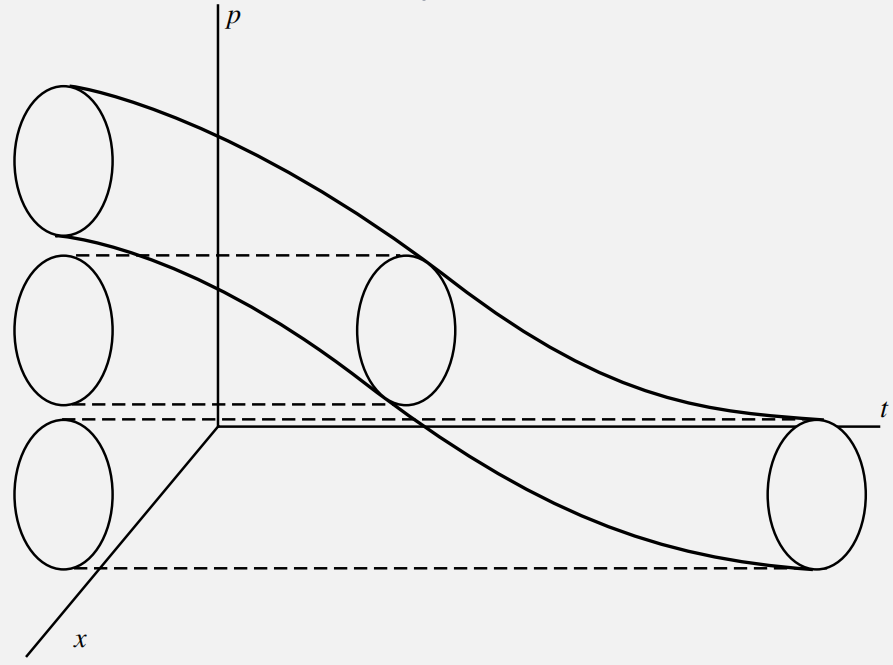
\includegraphics[height=2.15in,width=3.6in,viewport=0 0 893 655,clip]{Figures/Area-conservation-law-symplectic-flow.png}
%\caption{\fontsize{5.2pt}{4.2pt}\selectfont{\textrm{The Area conservation law for a sympletic flow.}}}%
\label{Area-conservation-law-symplectic-flow}
\end{figure}
\end{frame}

\begin{frame}
	\frametitle{相空间的粒子随时间演化:~积分}
	{\fontsize{8.5pt}{4.2pt}\selectfont{如果\textrm{Hamiltonian}可以表示为
	\begin{displaymath}
		\mathcal{H}=\mathbf{T}(p)+U(x)
	\end{displaymath}
	对相空间点$z=(p,x)$,则有
	\begin{displaymath}
		\begin{aligned}
			\dfrac{\mathrm{d}z}{\mathrm{d}t}=&\bigg(-\dfrac{\partial\mathcal{H}}{\partial x},\dfrac{\partial\mathcal{H}}{\partial p}\bigg)=\bigg(-\dfrac{\partial U(x)}{\partial x},\dfrac{\partial\mathbf{T}(p)}{\partial p}\bigg)\\
			=&\mathbf{J}\nabla\mathcal{H}(z)\equiv \tilde{\mathbf{T}}(z)+\tilde{U}(z)
		\end{aligned}
	\end{displaymath}
	其中
	\begin{displaymath}
		\begin{aligned}
			\tilde{\mathbf{T}}(z)=&\bigg(0,\dfrac{\partial\mathbf{T}(p)}{\partial p}\bigg)\\
			\tilde{U}(z)=&\bigg(\dfrac{\partial U(x)}{\partial x},0\bigg)
		\end{aligned}
	\end{displaymath}
	因此,粒子在相空间的解析形式为
	\begin{displaymath}
		\textcolor{blue}{z(t)=\mathrm{exp}(t\mathbf{J}\nabla\mathcal{H})[z(0)]=\mathrm{exp}[t(\tilde{\mathbf{T}}+\tilde{U})][z(0)]}
	\end{displaymath}
	$\mathrm{exp}(t\mathbf{J}\nabla\mathcal{H})$是时间演化算子,是保辛结构的,因此$\mathrm{exp}(t\tilde{\mathbf{T}})$和$\mathrm{exp}(t\tilde{U})$也是保辛结构的
}}
\end{frame}

\section{第一原理分子动力学简介}
\frame
{
	\frametitle{第一原理分子动力学\textrm{AIMD}中的近似}
	由于分子动力学模拟的复杂性,必须做出适当的近似。具体到第一原理分子动力学,一般有两类重要的近似:
	\begin{itemize}
		\item \textcolor{blue}{绝热近似\textrm{(adiabatic approximation)}}\\
			{\fontsize{6.2pt}{4.2pt}\selectfont{假设电子-原子核在能量层面上完全分离,彼此间没有能量传递}}
		\item \textcolor{blue}{\textrm{Born-Oppenheimer}近似}\\
			{\fontsize{6.2pt}{4.2pt}\selectfont{假设电子和原子核的运动完全解耦,对应每个时间步长的原子构型,电子可以实时处于基态\footnote{\fontsize{5.2pt}{4.2pt}\selectfont{\textrm{B-O}近似也是一种绝热近似,\textcolor{red}{但\textrm{B-O}近似下的绝热强调电子对核运动的瞬时响应}。讨论电子计算时,\textrm{B-O}近似下假设原子核是固定不动的;~在分子动力学讨论中,绝热近似强调的是电子-核运动在能量上的完整分离,而\textrm{B-O}近似则明确要求电子-核运动彼此完全解耦,且电子实时处于基态}}}}
	\end{itemize}
\begin{figure}[h!]
\centering
\vspace*{-0.25in}
%\hspace*{-10pt}
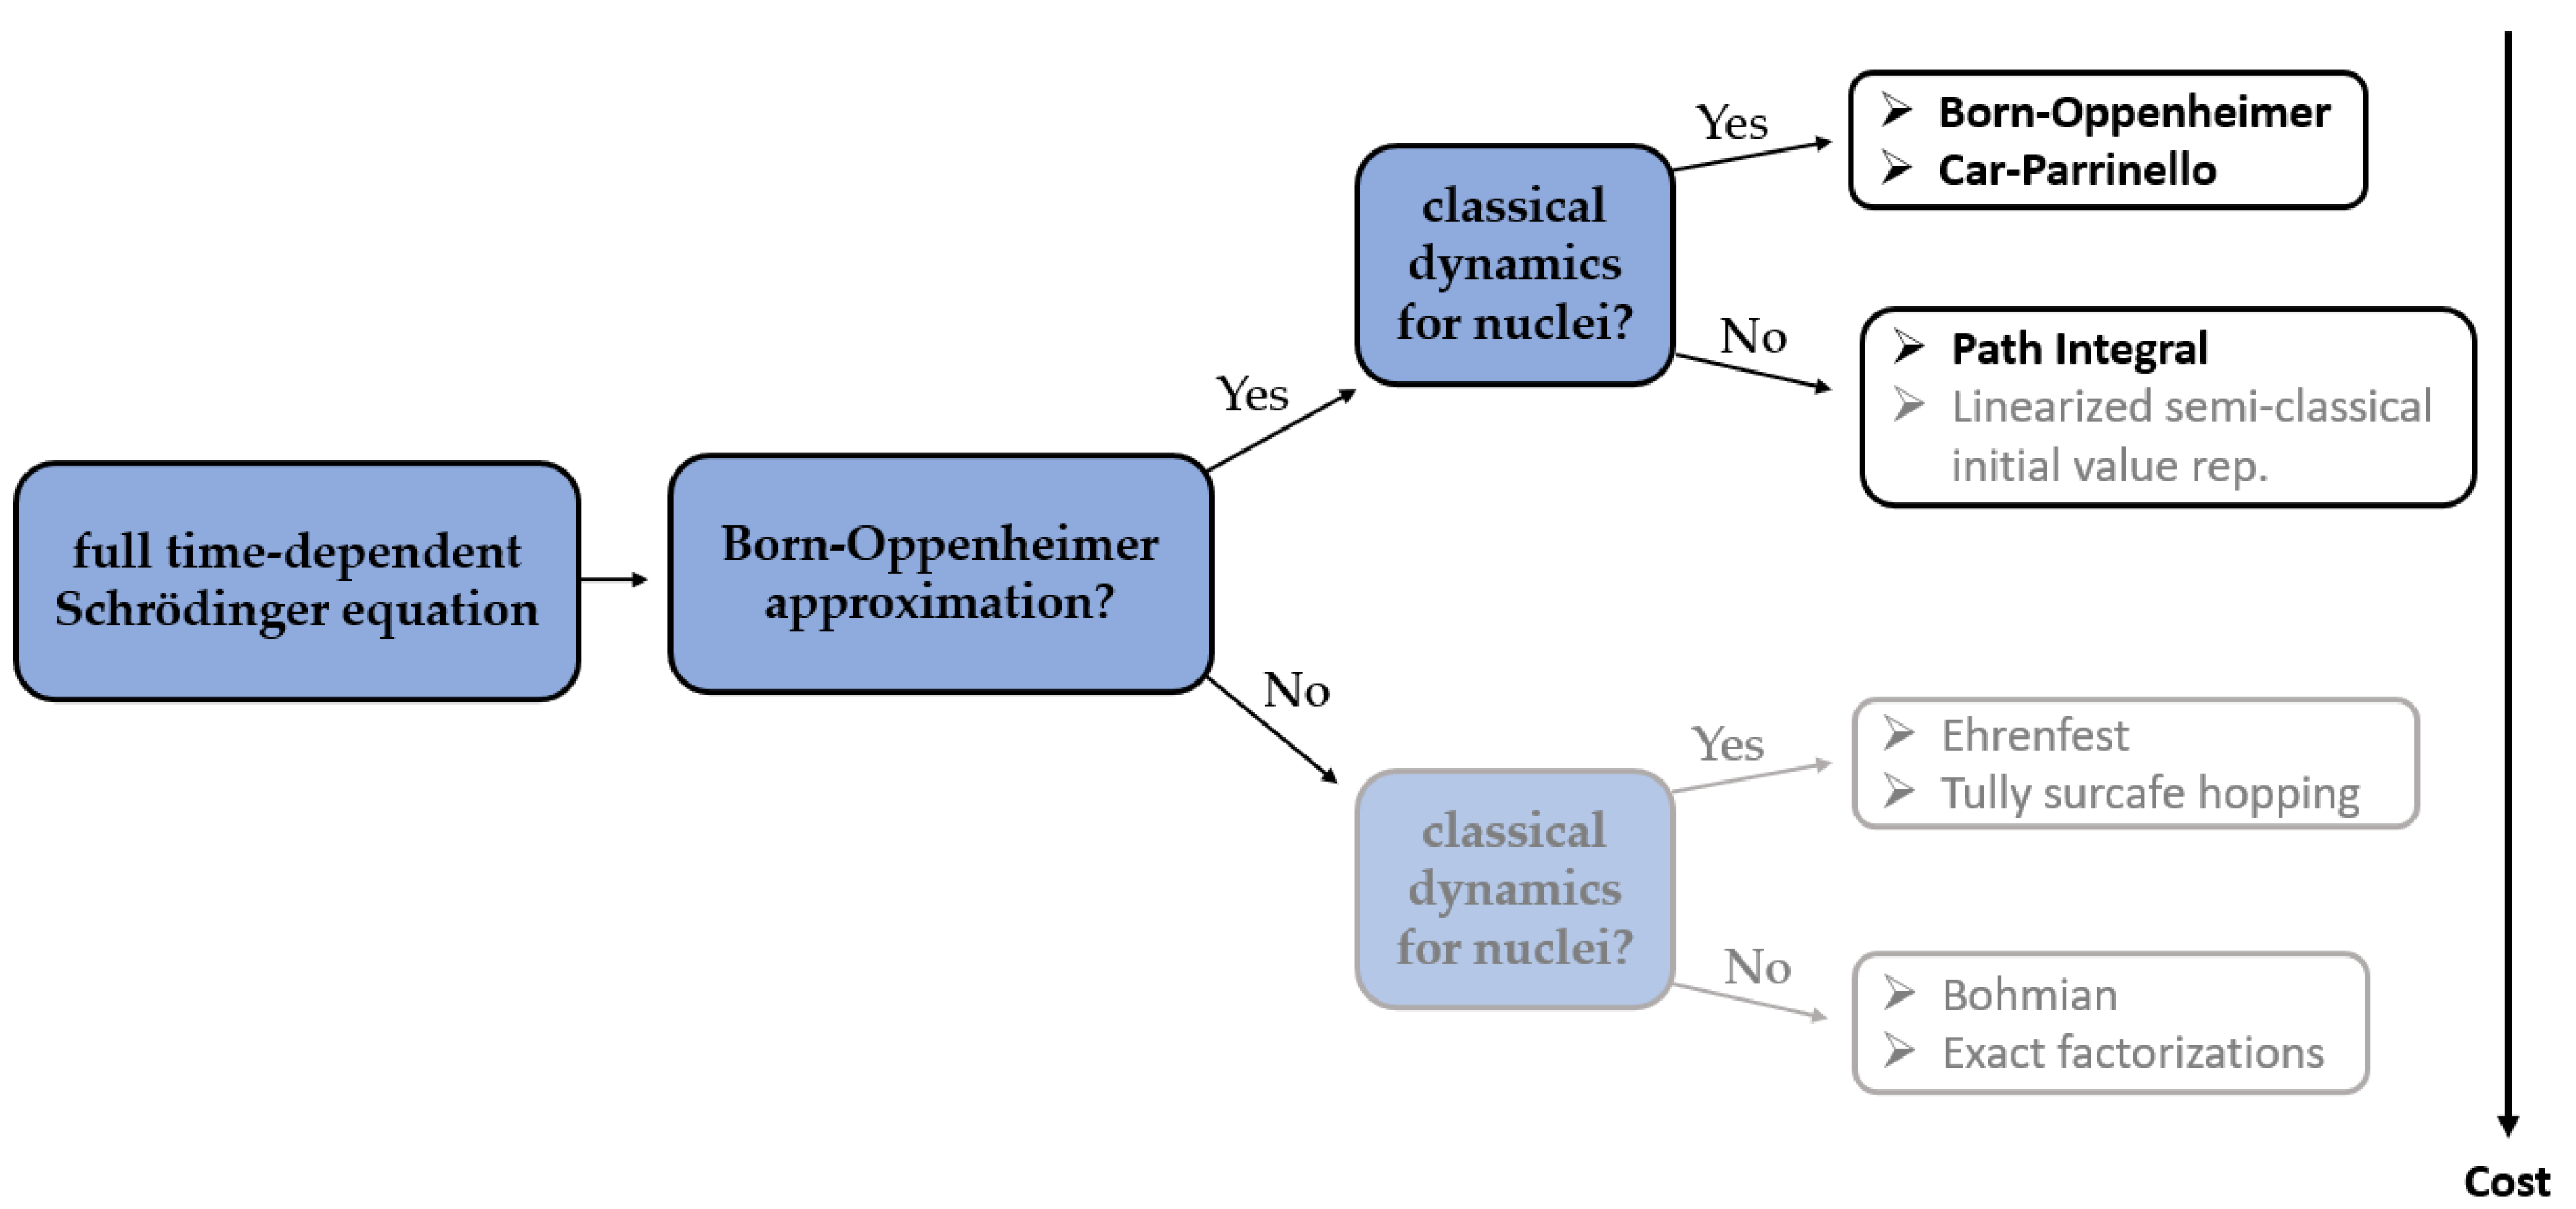
\includegraphics[height=1.55in,width=2.6in,viewport=0 0 440 230,clip]{Figures/Molecular-dynamics_Claaified.png}
%\caption{\fontsize{5.2pt}{4.2pt}\selectfont{\textrm{The major differences between the methods of aiMD simulations.}}}%
\label{Molecular-dynamics_Classified}
\end{figure}
}

\frame
{
	\frametitle{第一原理分子动力学}
	\begin{itemize}
		\item \textrm{AIMD}将电子结构与原子和经典轨迹计算在同一基础上完成
		\item 每个原子运动步的受力都是在电子结构计算基础上获得的
		\item 基于\textrm{B-O}方法:\\\textcolor{purple}{在计算原子运动径迹的每一步,都要求电子态都收敛到基态}
		\item 扩展的\textrm{Lagrangian}方法:~\textcolor{purple}{根据体系几何结构构造体系波函数}\\
			\textcolor{blue}{\textrm{Car-Parinello}}:\\
			平面波基,构成分子轨道\\
			\textcolor{blue}{\textrm{Atom-centered Density Matrix Progation~(ADMP)}}:\\
			原子中心基,构成密度矩阵
	\end{itemize}
	\textrm{AIMD}计算内容
	\begin{itemize}
		\item 可用于复杂体系的电子结构计算
		\item 几何结构优化(能量最小化)
		\item 描述系统演化
		\item 模拟时长规模$\approx{\mathrm{ps}}(10^{-12}\mathrm{s})$~(经典分子动力学 $\approx\mathrm{ns}(10^{-9}\mathrm{s})$)
	\end{itemize}
}


%\frame
%{
%	\frametitle{第一原理分子动力学的分类}
%\begin{figure}[h!]
%\centering
%\vspace*{-0.05in}
%%\hspace*{-10pt}
%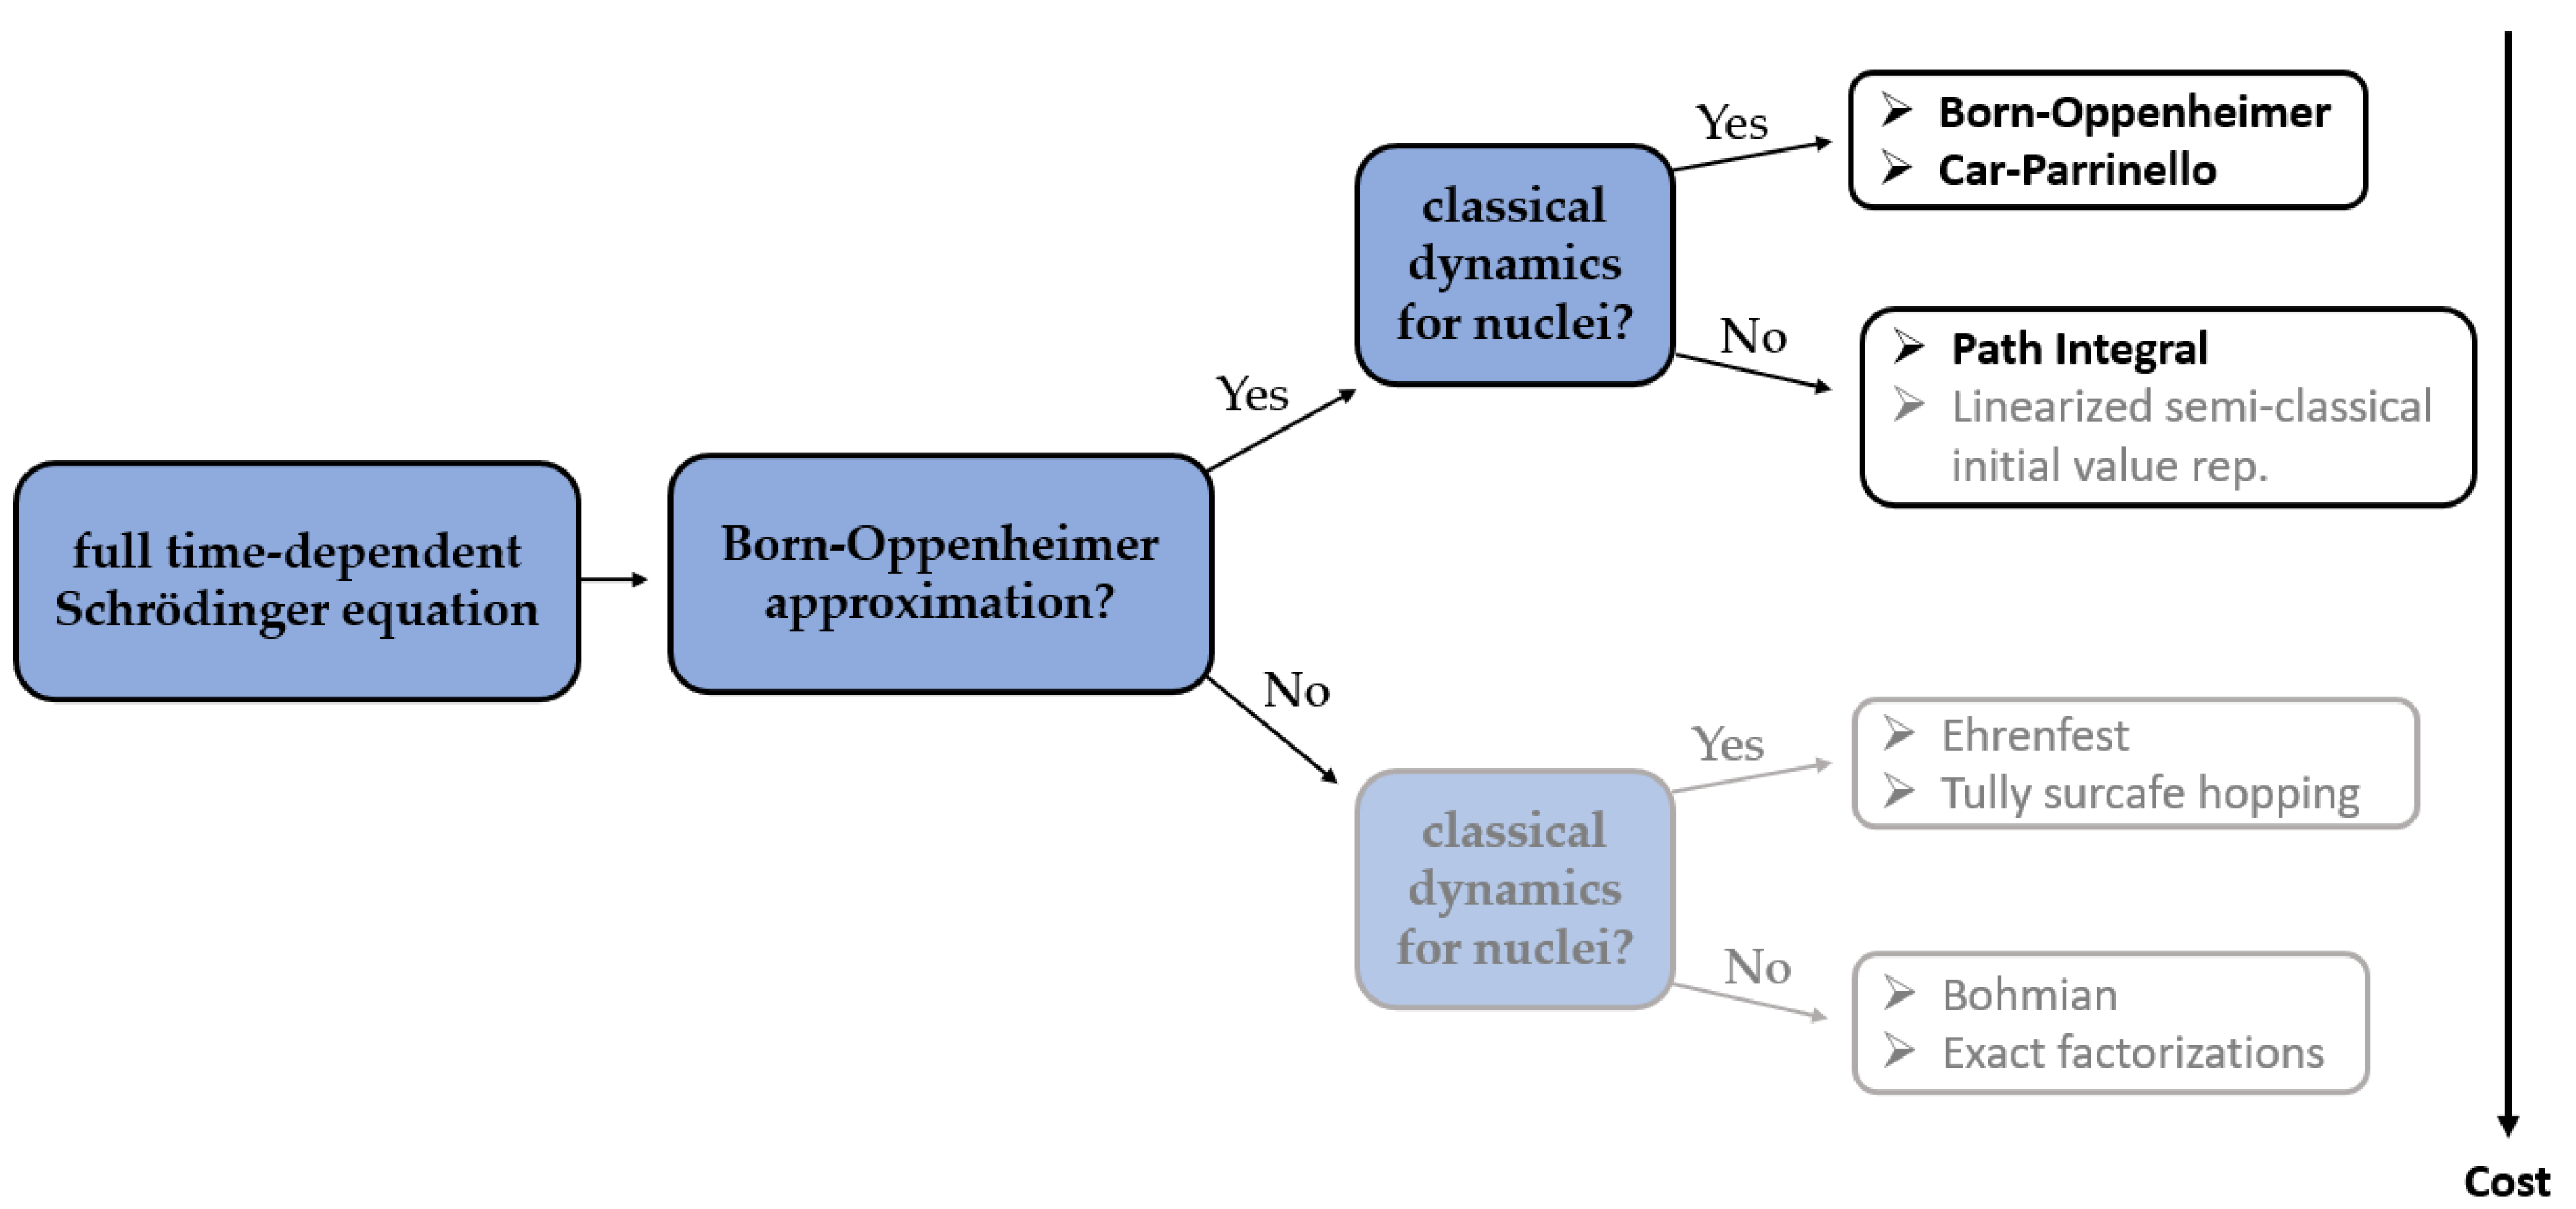
\includegraphics[height=2.3in,width=4.0in,viewport=0 0 440 230,clip]{Figures/Molecular-dynamics_Claaified.png}
%\caption{\fontsize{5.2pt}{4.2pt}\selectfont{\textrm{The major differences between the methods of aiMD simulations.}}}%
%\label{Molecular-dynamics_Claaified}
%\end{figure}
%}
%
\subsection{绝热近似:~{\rm Hellmann-Feynman}定理与电-声耦合}
%\frame
%{
%	\frametitle{第一原理分子动力学}
%	电子结构计算时,体系总能是基于\textrm{Born-Oppenheimer}近似得到,如果变化原子位置,可以得到体系总能随原子位置变化的规律\\
%	作为原子位置$\vec R_i$函数的电子态总能量$E(\vec R_1,\vec R_2,\cdots,\vec R_N)$称\textcolor{red}{势能面}~(\textrm{potential surface})
%
%	对于一套给定原子核位置$\mathbf{S}=(\vec R_1,\cdots,\vec R_N)$,$\vec R_i$表示第$i$个原子核的位置;~如果电子的基态波函数是$\psi_{\mathrm{G}}$则\\电子态能量为
%	\begin{displaymath}
%		E=\dfrac{\langle\psi_{\mathrm{G}}|\mathbf{H}(\mathbf{S})|\psi_{\mathrm{G}}\rangle}{\langle\psi_{\mathrm{G}}|\psi_{\mathrm{G}}\rangle}
%	\end{displaymath}
%作用在原子核$n$上的经典作用力,可由电子态能量对原子位置$\vec R_n$的梯度$\nabla_n$的负值给出
%\begin{displaymath}
%	\vec F_n=-\nabla_nE(\mathbf{S})=-\nabla_n\bigg[\dfrac{\langle\psi_{\mathrm{G}}|\mathbf{H}(\mathbf{S})|\psi_{\mathrm{G}}\rangle}{\langle\psi_{\mathrm{G}}|\psi_{\mathrm{G}}\rangle}\bigg]
%\end{displaymath}
%}
%
%\frame
%{
%	\frametitle{\textrm{Hellmann-Feynman}定理}
%	如果$\psi_{\mathrm{G}}$是\textrm{Hamiltonian}的本征态,有
%	\begin{displaymath}
%		\begin{aligned}
%			&(\langle\psi_{\mathrm{G}}|\psi_{\mathrm{G}}\rangle)^2\nabla_nE\\
%			=&\big[\langle(\nabla_n\psi_{\mathrm{G}}|\mathbf{H}|\psi_{\mathrm{G}}\rangle+\langle\psi_{\mathrm{G}}|(\nabla_n\mathbf{H})|\psi_{\mathrm{G}}\rangle+\langle\psi_{\mathrm{G}}|\mathbf{H}|(\nabla_n\psi_{\mathrm{G}})\rangle\big]\langle\psi_{\mathrm{G}}|\psi_{\mathrm{G}}\rangle\\
%			&-\langle\psi_{\mathrm{G}}|\mathbf{H}|\psi_{\mathrm{G}}\rangle\big[\langle(\nabla_n\psi_{\mathrm{G}})|\psi_{\mathrm{G}}\rangle+\langle\psi_{\mathrm{G}}|(\nabla_n\psi_{\mathrm{G}})\rangle\big]
%		\end{aligned}
%	\end{displaymath}
%	{\fontsize{6.2pt}{5.2pt}\selectfont{这里暂不考虑$\mathbf{H}$对原子核位置$\mathbf{S}$的依赖}}\\
%	\vskip 5pt
%	\textrm{Hellmann-Feynman}定理指出:~如果\textrm{Hamiltonian}量$\mathbf{H}$是\textrm{Hermitian}的,并且有
%	\begin{displaymath}
%		\mathbf{H}\psi_{\mathrm{G}}=E_{\mathrm{G}}\psi_{\mathrm{G}}
%	\end{displaymath}
%则上述表达式中,除了$\langle\psi_{\mathrm{G}}|(\nabla_n\mathbf{H})|\psi_{\mathrm{G}}\rangle$之外,等式右侧其余各项彼此抵消。由此得到能量梯度的表达式
%\begin{displaymath}
%	\nabla_nE=\dfrac{\langle\psi_{\mathrm{G}}|(\nabla_n\mathbf{H})|\psi_{\mathrm{G}}\rangle}{\langle\psi_{\mathrm{G}}|\psi_{\mathrm{G}}\rangle}
%\end{displaymath}
%}
%
\frame
{
	\frametitle{绝热近似}
	绝热近似下,电子-原子核的运动能量上完全分离,原子核运动的影响,在电子的本征态(本征值$E_i\{\mathbf{R}\}$,波函数$\Psi_i(\{\mathbf{r}\};\{\mathbf{R}\})$)中表现为含有原子核位置参数$\{\mathbf{R}\}$

	如果考虑核与电子体系,\textrm{Hamiltonian~}算符可以写成
	\begin{displaymath}
		\hat H=\hat T_N+\hat T_e+\hat U
	\end{displaymath}
	$U$是全部相互作用,可由\textcolor{blue}{电子坐标$\{\mathbf{r}\}$}和\textcolor{blue}{原子核位置$\{\mathbf{R}\}$}表示
\vskip 5pt
	电子态运动的本征态由下式确定
	\begin{displaymath}
		H_e(\mathbf{R})\psi_s(\{\mathbf{r};\mathbf{R}\})=E_s(\mathbf{R})\psi_s(\{\mathbf{r};\mathbf{R}\})
	\end{displaymath}
	这里$s=1,2,3,\cdots$
	电子运动\textrm{Hamiltonian}可由本征态表示为
	\begin{displaymath}
		\langle\psi_m(\mathbf{r};\mathbf{R})|\hat H_e(\mathbf{R})|\psi_n(\mathbf{r};\mathbf{R})\rangle=E_s(\mathbf{R})\delta_{mn}
	\end{displaymath}
	这里利用了电子本征态波函数的正交关系
	\begin{displaymath}
		\langle\psi_m(\mathbf{r};\mathbf{R})|\psi_n(\mathbf{r};\mathbf{R})\rangle=\delta_{mn}
	\end{displaymath}
}

\frame
{
	\frametitle{\textrm{Hellmann-Feynman}定理}
	根据电子波函数的正交关系,电子波函数对参数$\mathbf{R}$改变的响应有
	\begin{displaymath}
		\langle\dfrac{\partial}{\partial{\mathbf{R}_i}}\psi_m(\mathbf{r};\mathbf{R})|\psi_n(\mathbf{r};\mathbf{R})\rangle=-\langle\psi_m(\mathbf{r};\mathbf{R})|\dfrac{\partial}{\partial{\mathbf{R}_i}}\psi_n(\mathbf{r};\mathbf{R})\rangle
	\end{displaymath}
	对$m=n$有
	\textcolor{blue}{
		\begin{displaymath}
			\langle\psi_m(\mathbf{r};\mathbf{R})|\dfrac{\partial}{\partial{\mathbf{R}_i}}\psi_m(\mathbf{r};\mathbf{R})\rangle=\mbox{纯虚数}
		\end{displaymath} }
		类似地,\textrm{Schr\"odinger}方程对参数$\mathbf{R}$改变的响应有
		\begin{displaymath}
			\langle\dfrac{\partial\psi_m}{\partial{\mathbf{R}_i}}|H_e|\psi_n\rangle+\langle\psi_m|\dfrac{\partial H_e}{\partial{\mathbf{R}_i}}|\psi_n\rangle+\langle\psi_m|H_e|\dfrac{\partial\psi_n}{\partial{\mathbf{R}_i}}\rangle=\dfrac{\partial E_n}{\partial\mathbf{R}_i}\delta_{mn}
		\end{displaymath}
		注意到$\psi_m(\mathbf{r};\mathbf{R})$和$\psi_n(\mathbf{r};\mathbf{R})$是$H(\mathbf{R})$的本征态,本征值分别是$E_m(\mathbf{R})$和$E_n(\mathbf{R})$,因此有
		\begin{displaymath}
			\langle\psi_m|\dfrac{\partial H}{\partial{\mathbf{R}_i}}|\psi_n\rangle+[E_m-E_n]\langle\psi_m|H_e|\dfrac{\partial\psi_n}{\partial{\mathbf{R}_i}}\rangle=\dfrac{\partial E_n}{\partial\mathbf{R}_i}\delta_{mn}
		\end{displaymath}
}

\frame
{
	\frametitle{\textrm{Hellmann-Feynman}定理}
	当$m=n$时有\textrm{Hellmann-Feynman}定理
	\textcolor{purple}{
	\begin{displaymath}
		\langle\psi_m(\mathbf{r};\mathbf{R})|\dfrac{\partial H_e(\mathbf{R})}{\partial{\mathbf{R}_i}}|\psi_m(\mathbf{r};\mathbf{R})\rangle=\dfrac{\partial E_m(\mathbf{R})}{\partial\mathbf{R}_i}
	\end{displaymath}}
	电子态总能量$E(\mathbf{R})$与原子位置$\{\mathbf{R}_i\}$构成的函数称为\textcolor{red}{势能面}~(\textrm{potential surface})
	\vskip 8pt
	\textrm{Hellmann-Feynman}定理表明,对于确定的势能面,能量对位置导数(广义力)可通过波函数和算符$\partial H(\mathbf{R})/\partial\mathbf{R}_i$的期望值计算得到
	\vskip 5pt
	一般地,当势能面不包含任何简并态时,可以有\textrm{Epstein}广义\textrm{Hellmann-Feynman}定理
	\begin{displaymath}
		\hspace*{-10pt}
		\langle\psi_m(\mathbf{r};\mathbf{R})|\dfrac{\partial}{\partial{\mathbf{R}_i}}\psi_n(\mathbf{r};\mathbf{R})\rangle=\dfrac1{E_n(\mathbf{R})-E_m(\mathbf{R})}\langle\psi_m(\mathbf{r};\mathbf{R})|\dfrac{\partial H_e(\mathbf{R})}{\partial{\mathbf{R}_i}}|\psi_n(\mathbf{r};\mathbf{R})\rangle
	\end{displaymath}
}

\frame
{
	\frametitle{绝热近似下的原子受力}
	根据\textrm{Hellmann-Feynman}定理,在\textrm{Born-Oppenheimer}近似下,位于$\mathbf{R}_K$处的原子核的受力
	\begin{displaymath}
		\langle\psi(\mathbf{r};\mathbf{R})|\dfrac{\partial}{\partial{\mathbf{R}_K}}H_e(\mathbf{R})|\psi(\mathbf{r};\mathbf{R})\rangle=\dfrac{\partial E(\mathbf{R})}{\partial\mathbf{R}_K}
	\end{displaymath}
	这里\textrm{Hamiltonian}的梯度为
	\begin{displaymath}
		\dfrac{\partial}{\partial{\mathbf{R}_K}}H_e(\mathbf{R})=-\dfrac{\partial}{\partial{\mathbf{R}_K}}\sum_i\dfrac{Z_Ke^2}{\mathbf{r}_i-\mathbf{R}_K}+\dfrac{\partial}{\partial{\mathbf{R}_K}}\sum_{I(\neq K)}\dfrac{Z_IZ_Ke^2}{\mathbf{R}_I-\mathbf{R}_K}
	\end{displaymath}
	由此,原子受力可表示为
	\textcolor{red}{
	\begin{displaymath}
		\vec F_K=-\dfrac{\partial E}{\partial\mathbf{R}_K}=\int n(\mathbf{r};\mathbf{R})\dfrac{\partial}{\partial{\mathbf{R}_K}}\dfrac{Z_Ke^2}{\mathbf{r}_i-\mathbf{R}_K}\mathrm{d}\mathbf{r}-\dfrac{\partial}{\partial{\mathbf{R}_K}}\sum_{I(\neq K)}\dfrac{Z_IZ_Ke^2}{\mathbf{R}_I-\mathbf{R}_K}
	\end{displaymath}}
	原子核受力:~\textcolor{blue}{其余原子核的经典静电排斥}和\textcolor{purple}{电子的电荷密度分布}
}

\frame
{
	\frametitle{绝热近似下的核运动}
	绝热近似下,原子核-电子的波函数可以表示为
	\begin{displaymath}
		\Psi(\{\mathbf{r};\mathbf{R}\})=\sum_i\chi_{si}(\{\mathbf{R}\})\psi_i(\{\mathbf{r}\};\{\mathbf{R}\})
	\end{displaymath}
	原子核$\chi_{si}(\{\mathbf{R}\})$在电子形成的势能面$E_i(\{\mathbf{R}\})$上的运动方程
	\begin{displaymath}
		[T_N+E_i(\{\mathbf{R}\})-E_s]\chi_{si}(\{\mathbf{R}\})=-\sum_{ii^{\prime}}C_{ii^{\prime}}\chi_{si}(\{\mathbf{R}\})
	\end{displaymath}
	这里$T_n=-\frac12(\sum\limits_J\nabla_J^2/M_J)$,矩阵元$C_{ii^{\prime}}=A_{ii^{\prime}}+B_{ii^{\prime}}$
	\begin{displaymath}
		\begin{aligned}
			A_{ii^{\prime}}(\{\mathbf{R}\})=&\sum_J\frac1{M_J}\langle\psi_i(\{\mathbf{r}\};\{\mathbf{R}\})|\nabla_J|\psi_{i^{\prime}}(\{\mathbf{r}\};\{\mathbf{R}\})\rangle\nabla_J\\
			B_{ii^{\prime}}(\{\mathbf{R}\})=&\sum_J\frac1{2M_J}\langle\psi_i(\{\mathbf{r}\};\{\mathbf{R}\})|\nabla_J^2|\psi_{i^{\prime}}(\{\mathbf{r}\};\{\mathbf{R}\})\rangle\\
		\end{aligned}
	\end{displaymath}
	这里$\langle\psi_i(\{\mathbf{r}\};\{\mathbf{R}\})|\hat O|\psi_{i^{\prime}}(\{\mathbf{r}\};\{\mathbf{R}\})\rangle$表示对电子变量$\{\mathbf{r}\}$积分
}

\frame
{
	\frametitle{绝热近似下的核运动}
	绝热近似下,\textcolor{red}{将忽略矩阵$C_{ii^{\prime}}$的全部非对角元},可有
	\begin{itemize}
		\item \textcolor{blue}{电子能及时响应原子核的运动}
		\item \textcolor{blue}{电子由态$i\rightarrow i^{\prime}$的激发,不会影响原子核位置变量${\{\mathbf{R}\}}$}
		\item $A_{ii^{\prime}}=0$(波函数归一化要求)
		\item 核运动的势函数$U_i(\{\mathbf{R}\})=E_i(\{\mathbf{R}\})+B_{ii}(\{\mathbf{R}\})$
	\end{itemize}
	核运动方程
	\begin{displaymath}
		\left[ -\sum_J\frac1{2M_J}\nabla_J^2+U_i(\{\mathbf{R}\})-E_{ni} \right]\chi_{ni}(\{\mathbf{R}\})=0
	\end{displaymath}
这里$n=1,2,3,\cdots$

如果忽略$B_{ii}$的贡献,即绝热近似下冻声子(\textrm{frozen phonon})或微扰近似下的声子计算方案
}

\frame
{
	\frametitle{电-声耦合}
	电子-声子的来源:~\textcolor{blue}{$C_{ii^{\prime}}$的非对角元部分}
	\begin{itemize}
		\item $C_{ii^{\prime}}$的非对角元部分描述了\textcolor{red}{原子核运动(振动)引起电子在不同态间跃迁}
		\item $C_{ii^{\prime}}$的非对角元部分主要来自$A_{ii^{\prime}}$
			\begin{enumerate}
\setlength{\itemsep}{7pt}
				\item 电子波函数$\psi_i(\{\mathbf{r}\};\{\mathbf{R}\})$对原子核位置$\{\mathbf{R}_j\}$的梯度
				\item 梯度算符对原子核波函数$\chi_{si}(\{\mathbf{R}\})$的贡献
			\end{enumerate}
		\item 电子在态$i\rightarrow i^{\prime}$跃迁将会激发或吸收一个声子
	\end{itemize}
	根据\textrm{Epstein}推广的\textrm{Hellmann-Feynman}定理线性近似下有
	\begin{displaymath}
		\hspace*{-15pt}
		\langle\psi_i(\{\mathbf{r}\};\{\mathbf{R}\})|\nabla_J|\psi_i^{\prime}(\{\mathbf{r}\};\{\mathbf{R}\})\rangle=\frac{\langle\psi_i(\{\mathbf{r}\};\{\mathbf{R}\})|\tfrac{\nabla_V}{\nabla_{\mathbf{R}_J}}|\psi_{i^{\prime}}(\{\mathbf{r}\}:\{\mathbf{R}\})\rangle}{E_{i^{\prime}}(\{\mathbf{R}\})-E_i(\{\mathbf{R}\})}
	\end{displaymath}
}

\frame
{
	\frametitle{第一原理分子动力学:~\textrm{BOMD}}
	如果绝热近似和\textrm{Born-Oppenheimer}近似同时满足,称为\textrm{Born-Oppenheimer}分子动力学\textrm{(BOMD)}
	\begin{itemize}
		\item 原子核运动的势函数为$E[\{\psi_i\};\mathbf{R}]$,并且每个时间步长内,势函数对$\{\psi_i(\vec r)\}$取极小值\\
			\begin{displaymath}
				\begin{aligned}
					L_{\mathrm{BO}}(\{\psi_i\};~\mathbf{R},\dot{\mathbf{R}})=&\dfrac12\sum_{I=1}^NM_I\dot{\mathbf{R}}^2_I-\underset{\{\psi_i\}}{\textcolor{red}{\min}}~E[\{\psi_i\};\mathbf{R}]\\
					&+\sum_{ij}\Lambda_{ij}(\langle\psi_i|\psi_j\rangle-\delta_{ij})
				\end{aligned}
			\end{displaymath}
		\item 运动方程\textrm{(Equations of Motion,~EOM)}
			\begin{displaymath}
				\begin{aligned}
					\hspace*{-40pt}
					M_I\ddot{\mathbf{R}}_I=&-\nabla_{\mathbf{R}_I}\bigg[\underset{\{\psi_i\}}{\textcolor{red}{\min}}~E[\{\psi_i\};\mathbf{R}]\bigg|_{\{\langle\psi_i|\psi_j\rangle=\delta_{ij}\}}\bigg]\\
					=&\textcolor{purple}{-\dfrac{\partial E}{\partial\mathbf{R}_I}}\textcolor{blue}{+\sum_{i,j}\Lambda_{ij}\dfrac{\partial}{\partial \mathbf{R}_I}\langle\psi_i|\psi_j\rangle}\textcolor{magenta}{-2\sum_i\dfrac{\partial\langle\psi_i|}{\partial\mathbf{R}_I}\bigg[\dfrac{\delta E}{\delta\langle\psi_i|}-\sum_j\Lambda_{ij}|\psi_j\rangle\bigg]}
				\end{aligned}
			\end{displaymath}
	\end{itemize}
}

\frame
{
	\frametitle{第一原理分子动力学:~\textrm{BOMD}}
	\begin{itemize}
		\item $\textcolor{purple}{\dfrac{\partial E}{\partial\mathbf{R}_I}}$表示\textrm{Hellmann-Feynman}力$\vec F_{\mathrm{HF}}$
		\item $\textcolor{blue}{\sum\limits_{i,j}\Lambda_{ij}\dfrac{\partial}{\partial \mathbf{R}_I}\langle\psi_i|\psi_j\rangle}$是\textrm{Pulay}力$\vec F_{\mathrm{WF}}$\\
			{\fontsize{6.2pt}{4.2pt}\selectfont{源于电子波函数正交要求,且只有当基函数为局域函数(依赖于$\mathbf{R}$时)才有贡献}}
		\item $\textcolor{magenta}{\sum\limits_i\dfrac{\partial\langle\psi_i|}{\partial\mathbf{R}_I}\bigg[\dfrac{\delta E}{\delta\langle\psi_i|}-\sum\limits_j\Lambda_{ij}|\psi_j\rangle\bigg]}$表示非自洽电子态的影响$\vec F_{\mathrm{NSC}}$\\
			{\fontsize{6.2pt}{4.2pt}\selectfont{源自非局域基(如平面波),由于波函数非显式依赖$\mathbf{R}$,因此展开系数$c_{ij}(\mathbf{R})$依赖于原子核位置
			\begin{displaymath}
				\psi_i(\mathbf{R})=\sum\limits_jc_{ij}(\mathbf{R})\phi_i
			\end{displaymath}
			前面\textrm{MOE}中的系数\textrm{2}源于\textrm{K-S}轨道波函数为实数时的简化表示\\
			这一项的贡献比起$F_{\mathrm{HF}}$小很多,\textcolor{blue}{只要当$\psi_i(\mathbf{R})$是体系精确的电子的本征态波函数,该项就会消失}——换言之,只有非完全自洽的电子计算,才需要考虑该项的贡献。显然,所有数值计算中,都将存在不等式
	\begin{displaymath}
			0\leqslant-\dfrac{\delta E}{\delta\langle\psi_i|}+\sum_j\Lambda_{ij}|\psi_j\rangle=-\hat{H_{\mathrm{e}}}\langle\psi_j|+\sum_j\Lambda_{ij}|\psi_j\rangle
		\end{displaymath} }}
	\end{itemize}
}

\frame
{
	\frametitle{第一原理分子动力学:~\textrm{BOMD}}
	另一方面,如果忽略$\vec F_{\mathrm{WF}}$和$\vec F_{\mathrm{NSC}}$的贡献,仅对体系电子的非本征态波函数应用\textrm{Hellmann-Feynman}定理,得到的结果和精确计算的原子受力
	\begin{displaymath}
		\vec F=\vec F_{\mathrm{HF}}+\vec F_{\mathrm{WF}}+\vec F_{\mathrm{NSC}}
	\end{displaymath}
	计算相比,也只有微小的偏差
	\vskip 1.5pt
	这是因为在\textrm{DFT}框架下,能量是电荷密度的非线性函数,因此$H_{\mathrm{e}}$必须通过迭代求解;~而原子受力的误差则随电荷密度线性变化——这也解释了为什么一般\textrm{BOMD}计算的原子受力比体系总能要精确得多

	\vskip 5pt
	在\textrm{BOMD}中,\textrm{Born-Oppenheimer}近似下核与电子的运动完全解耦,在此基础上考虑绝热近似,将不再有对动力学模拟的时间步长限制,相比于其它\textrm{AIMD}方法,\textrm{BOMD}模拟允许的时间步长要长得多
}

\frame
{
	\frametitle{第一原理分子动力学:~\textrm{CPMD}}
	基于\textrm{Born-Oppenheimer}近似的原子-电子耦合的势能面计算,因每一原子步都需要完整的电子结构自洽迭代,故计算量非常可观。
\vskip 5pt
\textrm{1985}年,在\textrm{Car-Parrinello}给出的方案中,\textcolor{purple}{电子态将和原子核的运动一样,都用分子动力学算法处理}\\
在该方案中,\textcolor{blue}{体系的电子态并未能达到当前正电荷环境的真实基态,但体系总能可以与真实基态更为接近}\\
{\fontsize{6.2pt}{5.2pt}\selectfont{考虑\textcolor{blue}{电子态总能}(即\textcolor{red}{电子态有关能量}+\textcolor{magenta}{原子核静电相互作用能})是作为电子波函数$\psi_k$和原子核坐标$\mathbf{S}$的泛函
\begin{displaymath}
	E_{\mathrm{tot}}=E_{\mathrm{tot}}(\{\psi_k\},\mathbf{S})
\end{displaymath}
如果波函数可用一套基组$\{\chi_r\}$表示,即
\begin{displaymath}
	\psi_k(\vec r)=\sum_rC_{rk}\chi_r(\vec r)
\end{displaymath}
则体系总能可表示为
\begin{displaymath}
	E_{\mathrm{tot}}=E_{\mathrm{tot}}(\{C_{rk}\},\mathbf{S})
\end{displaymath}
考虑到基函数常常选择以原子核为坐标原点,因此也依赖于$\mathbf{S}$
}}\\
\textrm{Car-Parrinello}方法通过变量\underline{\textcolor{blue}{$\psi_k$(或$C_{rk}$)和原子核坐标$\mathbf{S}$}}来完成$E_{\mathrm{tot}}$的优化(确定$E_{\mathrm{tot}}$的极小值)
}

\frame
{
	\frametitle{第一原理分子动力学:~\textrm{CPMD}}
	{\fontsize{6.2pt}{5.2pt}\selectfont{到这里,能量最小化问题可以视为一个抽象的数学问题,原则上,任何一种最小化方法都适用(如模拟退火方法(\textrm{simulated annealing method}))}}
	\vskip 5pt
	\textrm{Car-Parrinello}要求原子核坐标随时间变化,还引入虚拟时间,要求波函数随虚拟时间变化,由此构造动态\textrm{Lagrangian}量\\
	{\fontsize{6.2pt}{5.2pt}\selectfont{\textrm{Lagrangian}量包括
	\begin{itemize}
		\item 电子态波函数$\{\psi_k\}$
		\item 原子核坐标$\{\vec R_i\}$
		\item 电子态波函数时间导数$\dot\psi_k$和原子核坐标时间导数$\{\dot{\vec R}_i\}$
	\end{itemize}}}
	电子态总能$E_{\mathrm{tot}}$是该\textrm{Lagrangian}量的势能,形式上这是一个经典力学的问题
	\begin{itemize}
		\item 在经典力学体系的运动方程中引入阻尼项贡献,则\\
			\textcolor{blue}{经过一段时间体系达到平衡态时,许可自由度的值对应体系经典势能达到最小值态时的取值}
		\item 在模拟体系在非零温下的运动时,可将阻尼项设为零
	\end{itemize}
}

\frame
{
	\frametitle{\textrm{CPMD}的\textrm{Lagrangian}}
	根据\textrm{Car-Parrinello~}定义的经典\textrm{Lagrangian~}量
			\begin{displaymath}
				\begin{aligned}
					L_{\mathrm{CP}}(\{\psi_i\};~\mathbf{R},\dot{\mathbf{R}})=&\textcolor{blue}{\dfrac12\mu\sum_i\langle\dot{\psi}_i|\dot{\psi}_i\rangle}+\dfrac12\sum_{I=1}^NM_I\dot{\mathbf{R}}^2_I\\
					-&\textcolor{red}{E}[\{\psi_i\};\mathbf{R}]\\
					&+\sum_{ij}\Lambda_{ij}(\langle\psi_i|\psi_j\rangle-\delta_{ij})
				\end{aligned}
			\end{displaymath}
%	{\fontsize{9.0pt}{5.2pt}\selectfont
%	\begin{displaymath}
%		L(\{\psi_k\},\{\vec R_n\})=\frac{\mu}2\sum_k\dot{\psi}_k^2+\sum_n\frac{M_n}2\dot{\vec R}_n^2-E_{\mathrm{tot}}(\{\psi_k\},\{\vec R_n\})+\sum_{kl}\Lambda_{kl}\langle\psi_k|\psi_l\rangle
%	\end{displaymath}}
%	这里$\mu$是一个很小的质量(可理解为虚拟电子质量);\\
%	$M_n$表示位置为$\vec R_n$处原子的真实质量;~\\
			{\fontsize{6.2pt}{4.2pt}\selectfont{在经典\textrm{Lagrangian}中考虑电子自由度,人为地引入了傀电子质量参数$\mu$和傀轨道速度$\dot{\psi}_i$}\\
	上式最后一项是要求波函数$\psi_k$正交的约束条件,$\Lambda_{kl}$是引入的\textrm{Lagrangian}乘子}
\vskip 5pt
{\fontsize{7.2pt}{5.2pt}\selectfont{$\mu$的选择原则:
		\begin{enumerate}
			\item $\mu\ll M$:~使得\textrm{Lagrangian}量中的\textcolor{blue}{电子动能项贡献足够小},因此波函数能随时适应原子核位置的变化
			\item $\mu$的选择兼顾效率与精度:\\
				一旦在运动方程中引入阻尼,电子和原子核的动能都将为零,体系总能(即\textrm{Lagrangian}量中的势能)达到极小值,但选择不同的$\mu$,计算过程中会有不同的收敛速度
		\end{enumerate}
	}}
}

\frame
{
	\frametitle{\textrm{CPMD}的运动方程}
由波函数正交约束,体系的\textrm{Euler-Lagrange~}运动方程可表示为
			{\fontsize{9.0pt}{4.2pt}\selectfont{
			\begin{displaymath}
				\begin{aligned}
					\mu\ddot{\psi}_i(\vec r,t)=&-\dfrac{\delta E}{\delta\langle\psi_i|}+\sum_j\Lambda_{ij}|\psi_j\rangle\\
					=&-\hat{H_{\mathrm{e}}}\langle\psi_j|+\sum_j\Lambda_{ij}|\psi_j\rangle\\
					M_I\ddot{\mathbf{R}}_I=&-\nabla_{\mathbf{R}_I}\bigg[E[\{\psi_i\};\mathbf{R}]\bigg|_{\{\langle\psi_i|\psi_j\rangle=\delta_{ij}\}}\bigg]\\
					=&\textcolor{purple}{-\dfrac{\partial E}{\partial\mathbf{R}_I}}\textcolor{blue}{+\sum_{i,j}\Lambda_{ij}\dfrac{\partial}{\partial \mathbf{R}_I}\langle\psi_i|\psi_j\rangle}
				\end{aligned}
			\end{displaymath}}}
%	\begin{displaymath}
%		\begin{aligned}
%			\mu\ddot{\psi}_k=&-\dfrac{\partial E_{\mathrm{tot}}}{\partial\psi_k}+2\sum_i\Lambda_{kl}(t)\psi_l(\vec r)\\
%			M_n\ddot{\vec R}_n&=-\dfrac{\partial E_{\mathrm{tot}}}{\partial\vec R_n}+\textcolor{red}{\sum_{kl}\Lambda_{kl}(t)\dfrac{\partial\langle\psi_k|\psi_l\rangle}{\partial\vec R_n}}
%		\end{aligned}
%	\end{displaymath}
	{\fontsize{6.5pt}{4.2pt}\selectfont{\begin{itemize}
		\item 电子态总能$E_{\mathrm{tot}}$是波函数$\psi_k$和原子核位置$\{\mathbf{R}_I\}$的函数 
			\vskip 3pt
		如果表示$\psi_k$的基函数不依赖原子核位置$\mathbf{R}_I$,则上述最后一个方程右侧最后一项消失
		\item $-\dfrac{\delta E}{\delta\langle\psi|}$表示经典力学框架下的电子受力,用来描述分子动力学范畴内电子自由度随原子核运动的情况
%			当波函数用基函数展开,电子运动方程可用展开系数表示为
%			\begin{displaymath}
%				\mu\ddot{\psi}_k=-\dfrac{\partial E_{\mathrm{tot}}}{\partial\psi_k}+2\sum_i\Lambda_{kl}(t)\sum_sS_{rs}(\vec r)C_{sl}
%			\end{displaymath}
		只要电子态波函数的基函数可由原子核位置确定,$\mu$的数值受基函数影响不大
	\end{itemize}}}
}

\frame
{
	\frametitle{\textrm{CPMD}的定态运动方程的求解}
	如果运动方程中引入阻尼项,则经过一段时间后,方程的解达到定态,前述运动方程等号左侧为零\footnote{\fontsize{6.2pt}{5.2pt}\selectfont{定态,意味着波函数和原子位置不再随时间变化}},因此可有
\begin{itemize}
	\item 电子态的运动方程与\textrm{Kohn-Sham}方程类似\\
		{\fontsize{6.2pt}{5.2pt}\selectfont{当前方程的矩阵元$\Lambda_{kl}$与\textrm{K-S}方程的能量本征值由$\varepsilon_k$对应}}
	\item \textrm{Lagrange}参数$\Lambda_{kl}$是时间相关的\\
		{\fontsize{6.2pt}{5.2pt}\selectfont{
		因此每个\textrm{MD}步必须重新计算$\Lambda_{kl}$,确保电子态波函数满足正交约束条件}}
	\item 应用具体的数值算法求解$\Lambda_{kl}$:~\\
	{\fontsize{6.5pt}{5.2pt}\selectfont
	应用\textrm{DFT~}框架下的\textrm{Hamiltonian}量,有
	\begin{displaymath}
		\psi_k(t+h)=2\psi_k(t)-\psi_k(t-h)-\dfrac{2h^2}{\mu}(H\psi_k-\sum_l\Lambda_{kl}\psi_l)
	\end{displaymath}
	该方程表明:~\textcolor{blue}{电子基态也可通过各种优化方法直接求解}}\\
		{\fontsize{6.2pt}{5.2pt}\selectfont{
			比如可用\textrm{Verlet~}算法计算;~\textrm{Car-Parrinello}建议用迭代\textrm{SHAKE}算法计算}}
	\item 对于搜索原子核的平衡位置问题,如果原子初始位置离平衡位置较远,很可能只得到体系的局域极小值\\
		{\fontsize{6.2pt}{5.2pt}\selectfont{使用模拟退火方法,使体系跃出局域极小点,搜索全局极小值}}
\end{itemize}
}

%\frame
%{
%	\frametitle{能量泛函的直接优化:~波函数的求解}
%	在\textrm{DFT~}框架下,有
%	{\fontsize{9.0pt}{5.2pt}\selectfont
%	\begin{displaymath}
%		\psi_k(t+h)=2\psi_k(t)-\psi_k(t-h)-\dfrac{2h^2}{\mu}(H\psi_k-\sum_l\Lambda_{kl}\psi_l)
%	\end{displaymath}}
%%	该方程表明:~\textcolor{blue}{电子基态也可通过各种优化方法直接求解}
%	每个时间步$t$,\textrm{Car-Parrinello~}采用\textrm{SHAKE~}算法迭代确定$\psi_k(t)$
%}
%
\frame
{
	\frametitle{\textrm{CPMD}的原子核受力}
	原子核运动方程的求解主要围绕电子态总能对原子位置$\vec R_i$的求导,对求导有贡献的共三部分
	\begin{itemize}
		\item 原子核之间的\textrm{Coulomb}相互作用:\\
			与原子核间距离反比:~$1/R_{ij}~\quad\vec R_{ij}=|\vec R_i-\vec R_j|$
		\item 电子\textrm{Hamiltonian}中包括的电子与核之间的\textrm{Coulomb}吸引势\\
			与原子核位置有关:~$\vec R_i$
		\item 基函数$\chi_r$对原子核位置$\vec R_i$的依赖\\
			当基函数的中心选定在原子核$\vec R_i$上时,原子核位置的变化会引起\textrm{Fock}矩阵和重叠矩阵的变化\\
	{\fontsize{7.2pt}{5.2pt}\selectfont{因原子核位置变化引起基函数改变的贡献称为\textcolor{blue}{\textrm{Pulay}力}}}
	\end{itemize}
	\textrm{Car-Parrinello}方法得到的结果与二体势(力场)方法结果等价
	\vskip 5pt
	计算得到位于$\vec R_i$的原子核受力,用于描述\textrm{Verlet}模拟原子核的运动状态
}

\frame
{
	\frametitle{\textrm{H}原子\textrm{AIMD}计算示例}
\begin{figure}[h!]
	\vspace{-0.25in}
\centering
%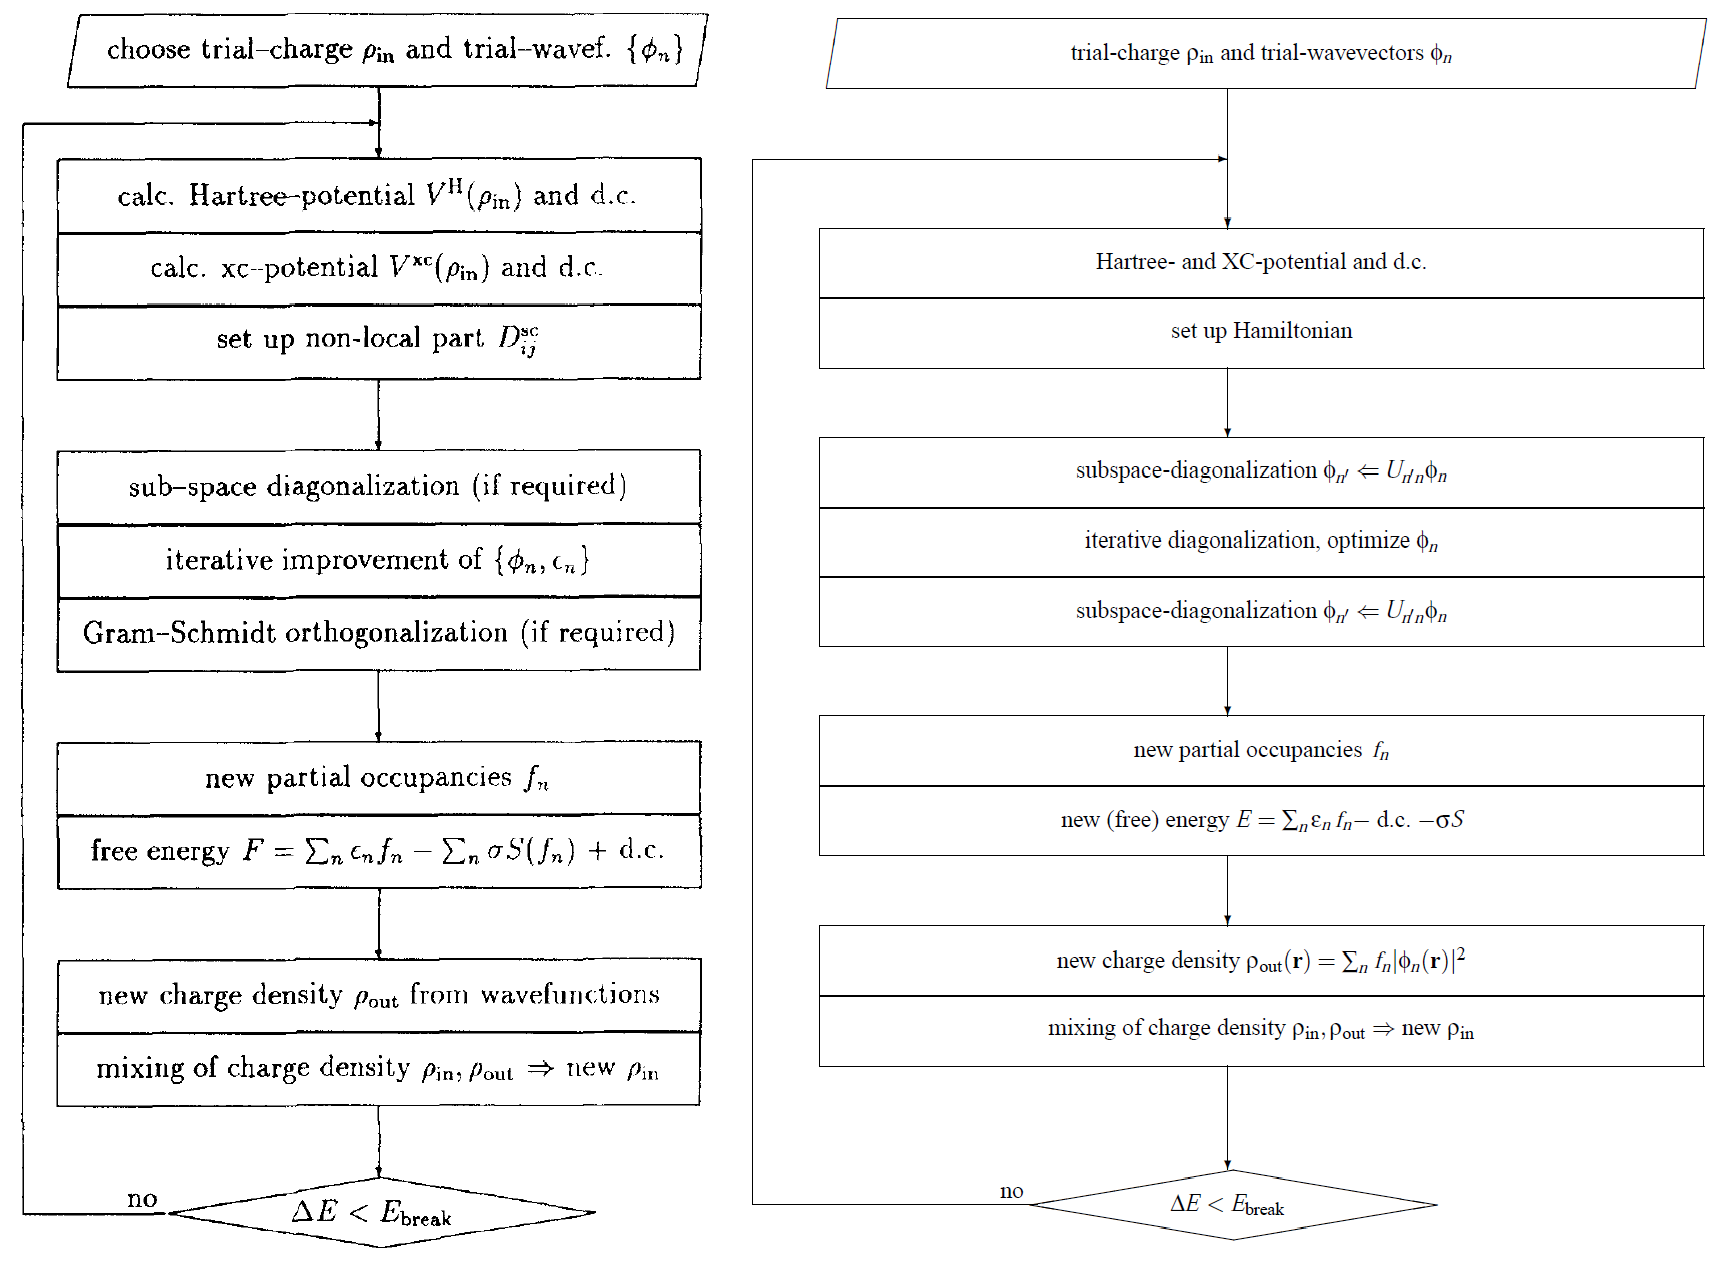
\includegraphics[height=2.7in,width=4.0in,viewport=0 0 1300 960,clip]{Figures/VASP_procedure-full.png}
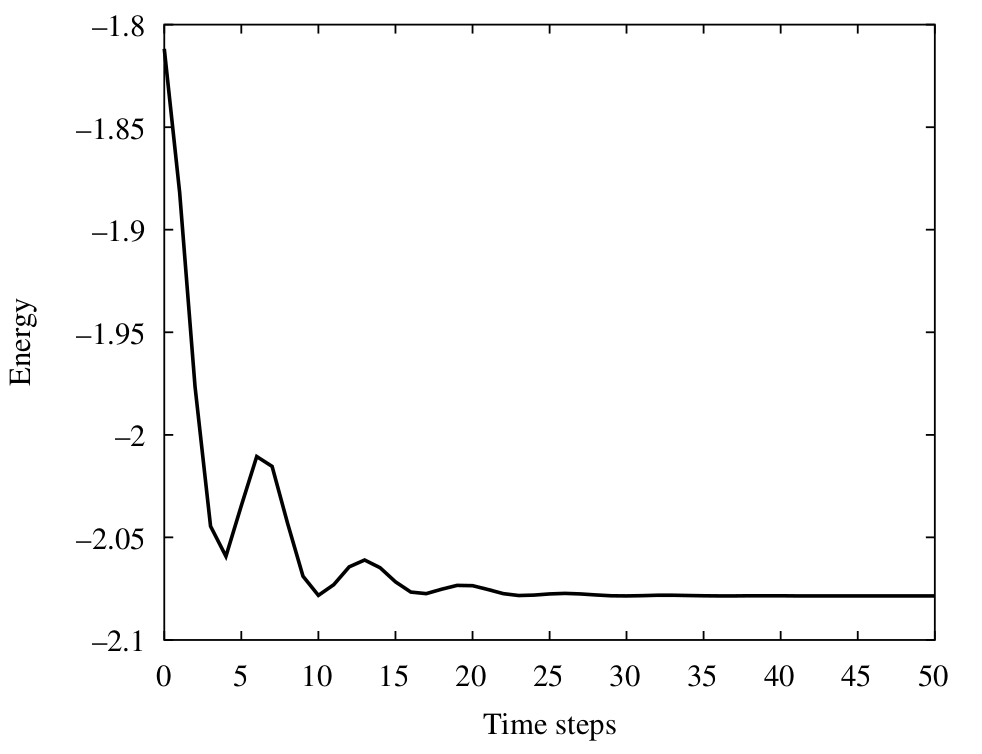
\includegraphics[height=1.5in,width=1.9in,viewport=0 0 740 600,clip]{Figures/Ab-initio-Ene.png}\\
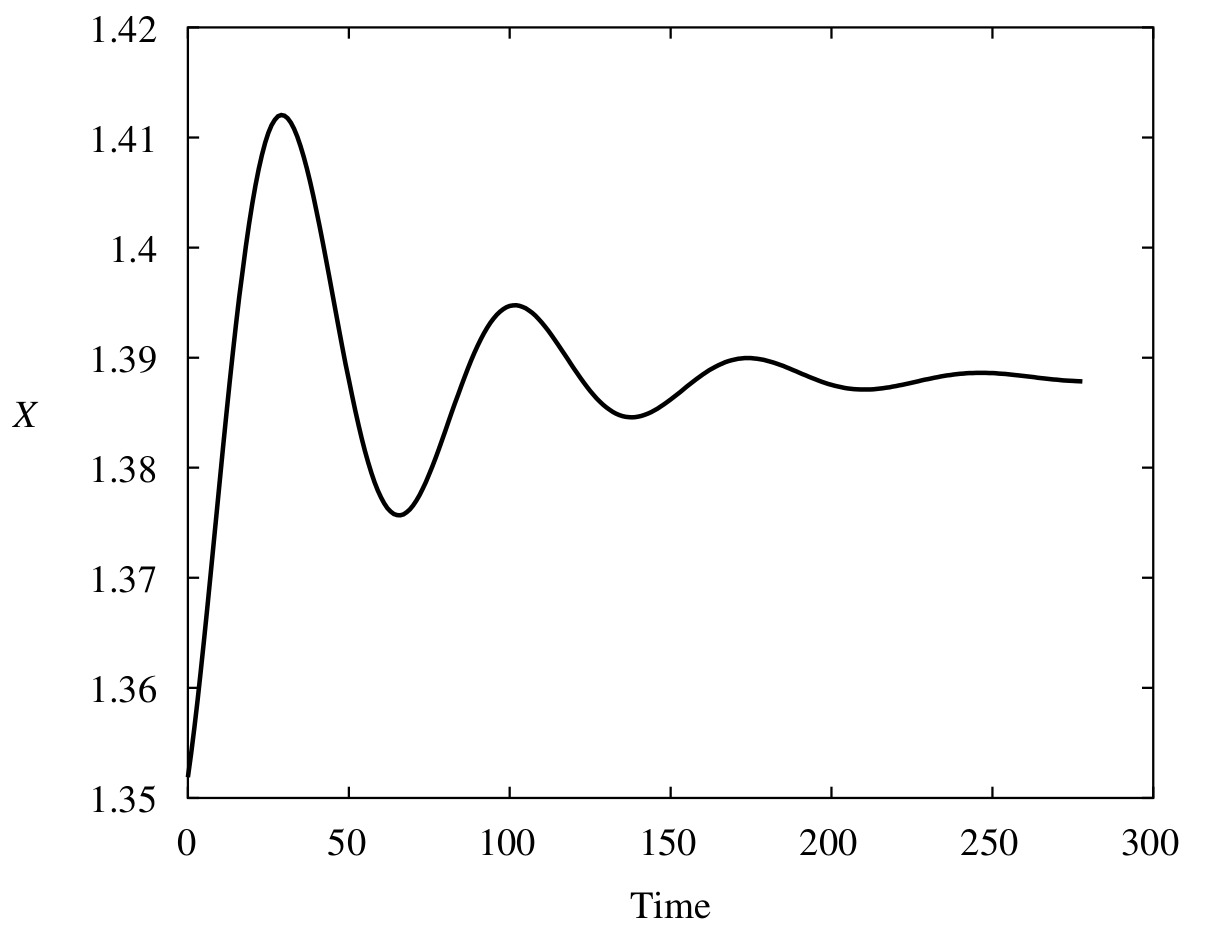
\includegraphics[height=1.5in,width=1.9in,viewport=0 0 1200 950,clip]{Figures/MD_H-R-rel.png}
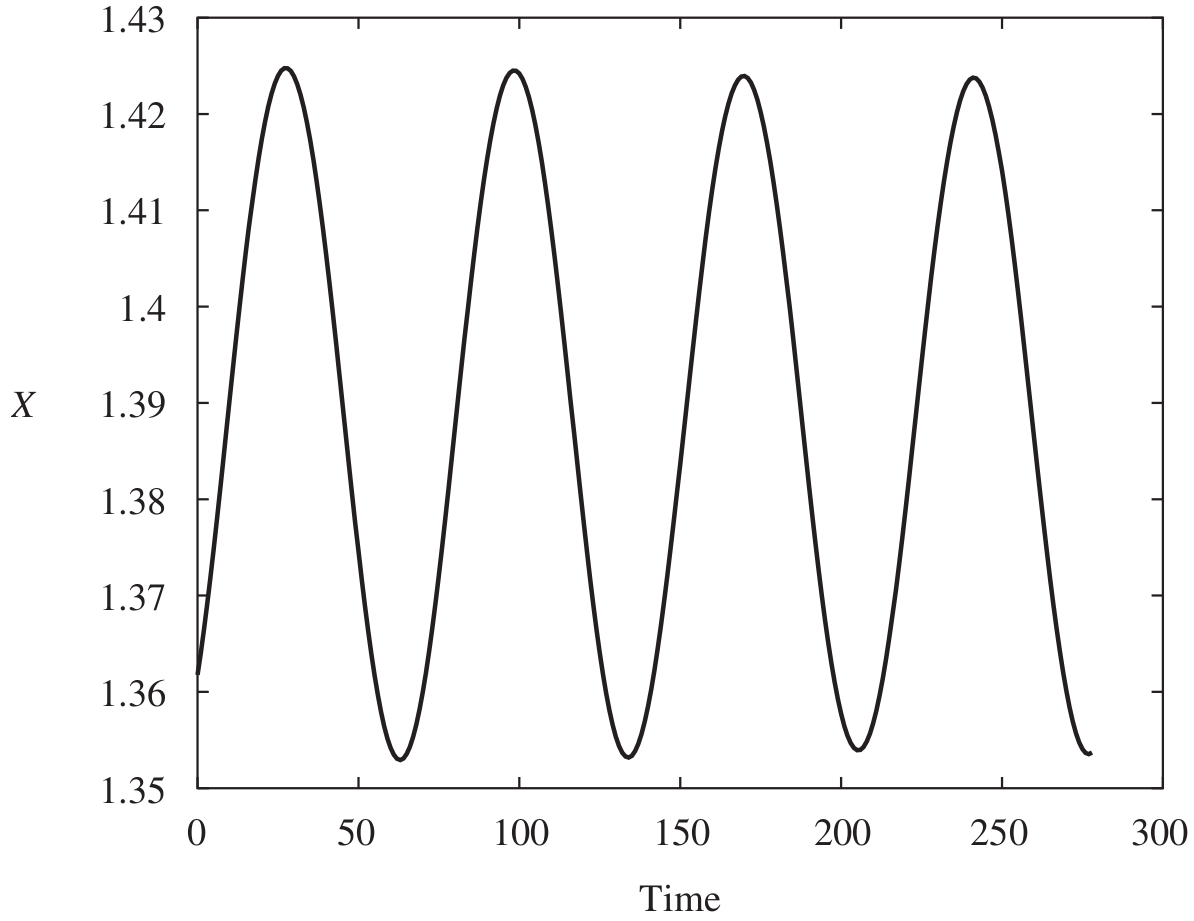
\includegraphics[height=1.5in,width=1.9in,viewport=0 0 1200 950,clip]{Figures/MD_H-R-MD.png}
\caption{\tiny \textrm{The Flow of calculation for the AIMD.}}%(与文献\cite{EPJB33-47_2003}图1对比)
\label{PAW_AIMD}
\end{figure} 
}


\frame
{
	\frametitle{波函数正交对计算的影响}
	{\fontsize{9.0pt}{5.2pt}\selectfont
	\textrm{Verlet}算法计算电子态波函数的运动方程
	\begin{displaymath}
		|\tilde\psi_k(t+h)\rangle=2|\psi_k(t)\rangle-|\psi_k(t-h)\rangle-\dfrac{2h^2}{\mu}(H|\psi_k(t)\rangle-\sum_l\Lambda_{kl}\psi_l)
	\end{displaymath}}
	当体系含有多个电子,\textrm{Langrage}乘子确保电子波函数彼此正交\\%,可有
	{\fontsize{7.0pt}{5.2pt}\selectfont
	实际上,存在多种正交方案
	\begin{itemize}
		\item 一次\textrm{unitary}变换产生一套正交轨道
			\begin{displaymath}
				\psi_k^{\prime}=\sum_lU_{kl}\psi_l
			\end{displaymath}
			这里基组$\{\psi_k^{\prime}\}$是正交的
		\item 一次波函数的\textrm{unitary}变化伴随\textrm{Lagtange}乘子的一次类似变换
			\begin{displaymath}
				\Lambda_{kl}^{\prime}=\sum_{mn}U_{km}^{\dagger}\Lambda_{mn}U_{nl}
			\end{displaymath}
	\end{itemize}
	不同的正交方案对应张开的空间相同,但张开空间的函数有所旋转
%	\begin{displaymath}
%		|\psi_k(t+h)\rangle=|\tilde\psi_k(t+h)\rangle+\sum_lX_{kl}|\psi_l(t)\rangle
%	\end{displaymath}
}\\
%	其中,{\fontsize{9.0pt}{5.2pt}\selectfont$X_{kl}=\dfrac{2h^2}{\mu}\Lambda_{kl}$},由此$|\psi_k(t+h)\rangle$正交\\
%	$X_{ij}$要求关于$\mathbf{X}$的矩阵方程
	{\fontsize{8.0pt}{5.2pt}\selectfont
	\textcolor{purple}{不同的旋转方式(不同的正交方案)会对\textrm{Verlet}算法的执行效率产生很大的影响}
%	\begin{displaymath}
%		\mathbf{X}\mathbf{X}^{\dag}+\mathbf{X}\mathbf{B}+\mathbf{B}^{\dag}\mathbf{X}^{\dag}=\mathbf{I}-\mathbf{A}
%	\end{displaymath}
}
%	能通过以下迭代快速收敛,这里{\fontsize{9.0pt}{5.2pt}\selectfont$A_{kl}=\langle\tilde\psi_k(t+h)|\tilde\psi_l(t+h)\rangle$},{\fontsize{9.0pt}{5.2pt}\selectfont$B_{kl}=\langle\psi_k(t)|\tilde\psi_l(t+h)\rangle$}
	{\fontsize{9.0pt}{5.2pt}\selectfont
%	\begin{displaymath}
%		\mathbf{X}^{(n+1)}=\frac12[\mathbf{I}-\mathbf{A}+\mathbf{X}^{(n)}(\mathbf{I}-\mathbf{B})+\mathbf{X}^{(n)}(\mathbf{I}-\mathbf{B}^{\dag})-\mathbf{X}^{n}\mathbf{X}^{(n){\dag}}]
%		\end{displaymath}
}
%	取初始{\fontsize{9.0pt}{5.2pt}\selectfont$\mathbf{X}=\frac12(\mathbf{I}-\mathbf{A})$}
}

%\subsection{电子态能量的最小化}
\frame[allowframebreaks]
{
	\frametitle{\textrm{CPMD}与平面波基}
	\begin{itemize}
		\item 推导总能对轨道自由度的受力
	{\fontsize{6.2pt}{5.2pt}\selectfont{
			\begin{displaymath}
				\begin{aligned}
					\dfrac{\partial E_{\mathrm{total}}}{\partial c_j^{\ast}(\vec K)}=&\dfrac{K^2}2c_j(\vec K)+\sum_{\vec K^{\prime}}V_{\mathrm{loc}}^{\ast}(\vec K-\vec K^{\prime})c_j(\vec K^{\prime})\\
					&+\sum_n\sum_{lm}F_{jlm}^n\mathrm{e}^{-\mathrm{i}\vec K\cdot\vec R_n}Y_{lm}(\hat{\vec K})h_{lm}^np_m^l(K)
				\end{aligned}
			\end{displaymath}
			这里$V_{\mathrm{loc}^{\mathrm{all}}}$是总局域势
			\begin{displaymath}
				V_{loc}(\vec K)=\sum_n\Delta V_{\mathrm{loc}}(\vec K)+V_{\mathrm{xc}}(\vec K)+4\pi\dfrac{n_{\mathrm{tot}}(\vec K)}{K^2}
			\end{displaymath}
		}}
		\item 推导总能对原子核的受力:\\
{\fontsize{6.2pt}{5.2pt}\selectfont{
			总能对原子位置坐标的梯度包括
			\begin{itemize}
{\fontsize{6.2pt}{5.2pt}\selectfont{
				\item 局域赝势部分的贡献
					\begin{displaymath}
						\nabla_{\vec R_n}E_{\mathrm{local}}=-\Omega\sum_{\vec K}\mathrm{i}\vec KV_{\mathrm{local,n}}(\vec K)\mathrm{e}^{-\mathrm{i}\vec K\cdot\vec R_n}n^{\ast}(\vec K)
					\end{displaymath}
				\item 非局域赝势部分的贡献
					\begin{displaymath}
						\nabla_{\vec R_n}E_{\mathrm{nonlocal}}=\sum_jf_j\sum_{l,m\varepsilon n}[(F_{jlm}^n)^{\ast}h_{lm}^n\nabla_{\vec R_n}F_{jlm}^n+\nabla_{\vec R_n}(F_{lm}^n)^{\ast}h_{lm}^nF_{lm}^n]
					\end{displaymath}
				\item 电子-核静电相互作用部分的贡献
					\begin{displaymath}
						\nabla_{\vec R_n}E_{\mathrm{ES}}=-\Omega\sum_{\vec K}\mathrm{i}\vec K\dfrac{n_{\mathrm{tot}}}{K^2}n_{\mathrm{core}}^n(\vec K)\mathrm{e}^{-\mathrm{i}\vec K\cdot\vec R_n}+\nabla_{\vec R_n}E_{\mathrm{ovrl}}
\end{displaymath}
				}}
			\end{itemize}
			其中
			\begin{displaymath}
				\nabla_{\vec R_n}F_{lm}^n=-\dfrac1{\sqrt{\Omega}}\sum_{\vec K}\mathrm{i}\vec K\mathrm{e}^{-\mathrm{i}\vec K\cdot\vec R_n}c_j^{\ast}(\vec K)Y_{lm}(\hat{\vec K})p_{lm}^l(\vec K)
			\end{displaymath}
			\begin{displaymath}
				\begin{aligned}
					\nabla_{\vec R_n}E_{\mathrm{ovrl}}=&\sideset{}{^{\prime}}\sum_{n^{\prime}}\sum_{\vec L}\bigg\{\dfrac{Z_nZ_{n^{\prime}}}{|\vec R_n-\vec R_{n^{\prime}}-\vec L|^3}\mathrm{erfc}\bigg[\dfrac{|\vec R_n-\vec R_{n^{\prime}}-\vec L|}{\sqrt{2(\xi_n^2+\xi_{n^{\prime}}^2)}}\bigg]\\
					&+\dfrac2{\sqrt{\pi}}\dfrac1{\sqrt{\xi_n^2+\xi_{n^{\prime}}^2}}\dfrac{Z_nZ_{n^{\prime}}}{|\vec R_n-\vec R_{n^{\prime}}-\vec L|^2}\mathrm{exp}\bigg[\dfrac{|\vec R_n-\vec R_{n^{\prime}}-\vec L|}{\sqrt{2(\xi_n^2+\xi_{n^{\prime}}^2)}}\bigg]\bigg\}\\
					&\times(\vec R_n-\vec R_{n^{\prime}}-\vec L)
				\end{aligned}
			\end{displaymath}
		}}
	\end{itemize}

}

\frame
{
	\frametitle{\textrm{CPMD}方法总结}
	\textrm{Car-Parinello~}方法基本思想
	\begin{itemize}
		\item 只对原子核位置考虑受力$-\dfrac{\partial E_{\mathrm{tot}}}{\partial\vec R_n}$作用
		\item 电子结构是通过某种最小化方法确定能量泛函$E_{\mathrm{tot}}[\rho(\vec r)]$的极值得到,而非\textrm{Born-Oppenheimer}近似下的自洽迭代
		\item \textrm{Verlet}算法确定核位移过程中,并不要求在每一步核位移时,电子步充分弛豫到当前结构的基态
	\end{itemize}
	在\textrm{Car-Parinello}方法中,电子结构的计算变成经典的优化问题:~电子密度迭代过程中,约束条件下最小化问题
	\begin{itemize}
		\item 电子本征态波函数彼此正交约束下迭代对角化(内循环):\\
			\textcolor{blue}{子空间旋转}:~不同的正交化方法对迭代计算的影响
		\item 电荷密度混合过程中电荷数守恒约束(外循环)
			\begin{displaymath}
				\sum\limits_{j=0}^i a_j=1
			\end{displaymath}
	\end{itemize}
}

%\frame
%{
%	\frametitle{统计系综}
%	系综(\textrm{Ensembles})是在一定的宏观条件下,由大量微观粒子组成的性质和结构完全相同的、处于各种运动状态的、各自独立的系统整体的集合\footnote{\fontsize{4.2pt}{2.2pt}\selectfont{简言之,系综是系统的集合(\textcolor{magenta}{系统}:~宏观相同,微观不同)。}}。\\
%	应用\textrm{Verlet}算法,完成单粒子运动的数值积分,可以得到动力学体系的\textrm{Hamiltonian}对应的能量,进而应用统计力学的统计系综,获得宏观体系的物理量
%\begin{figure}[h!]
%\centering
%\vspace*{-0.20in}
%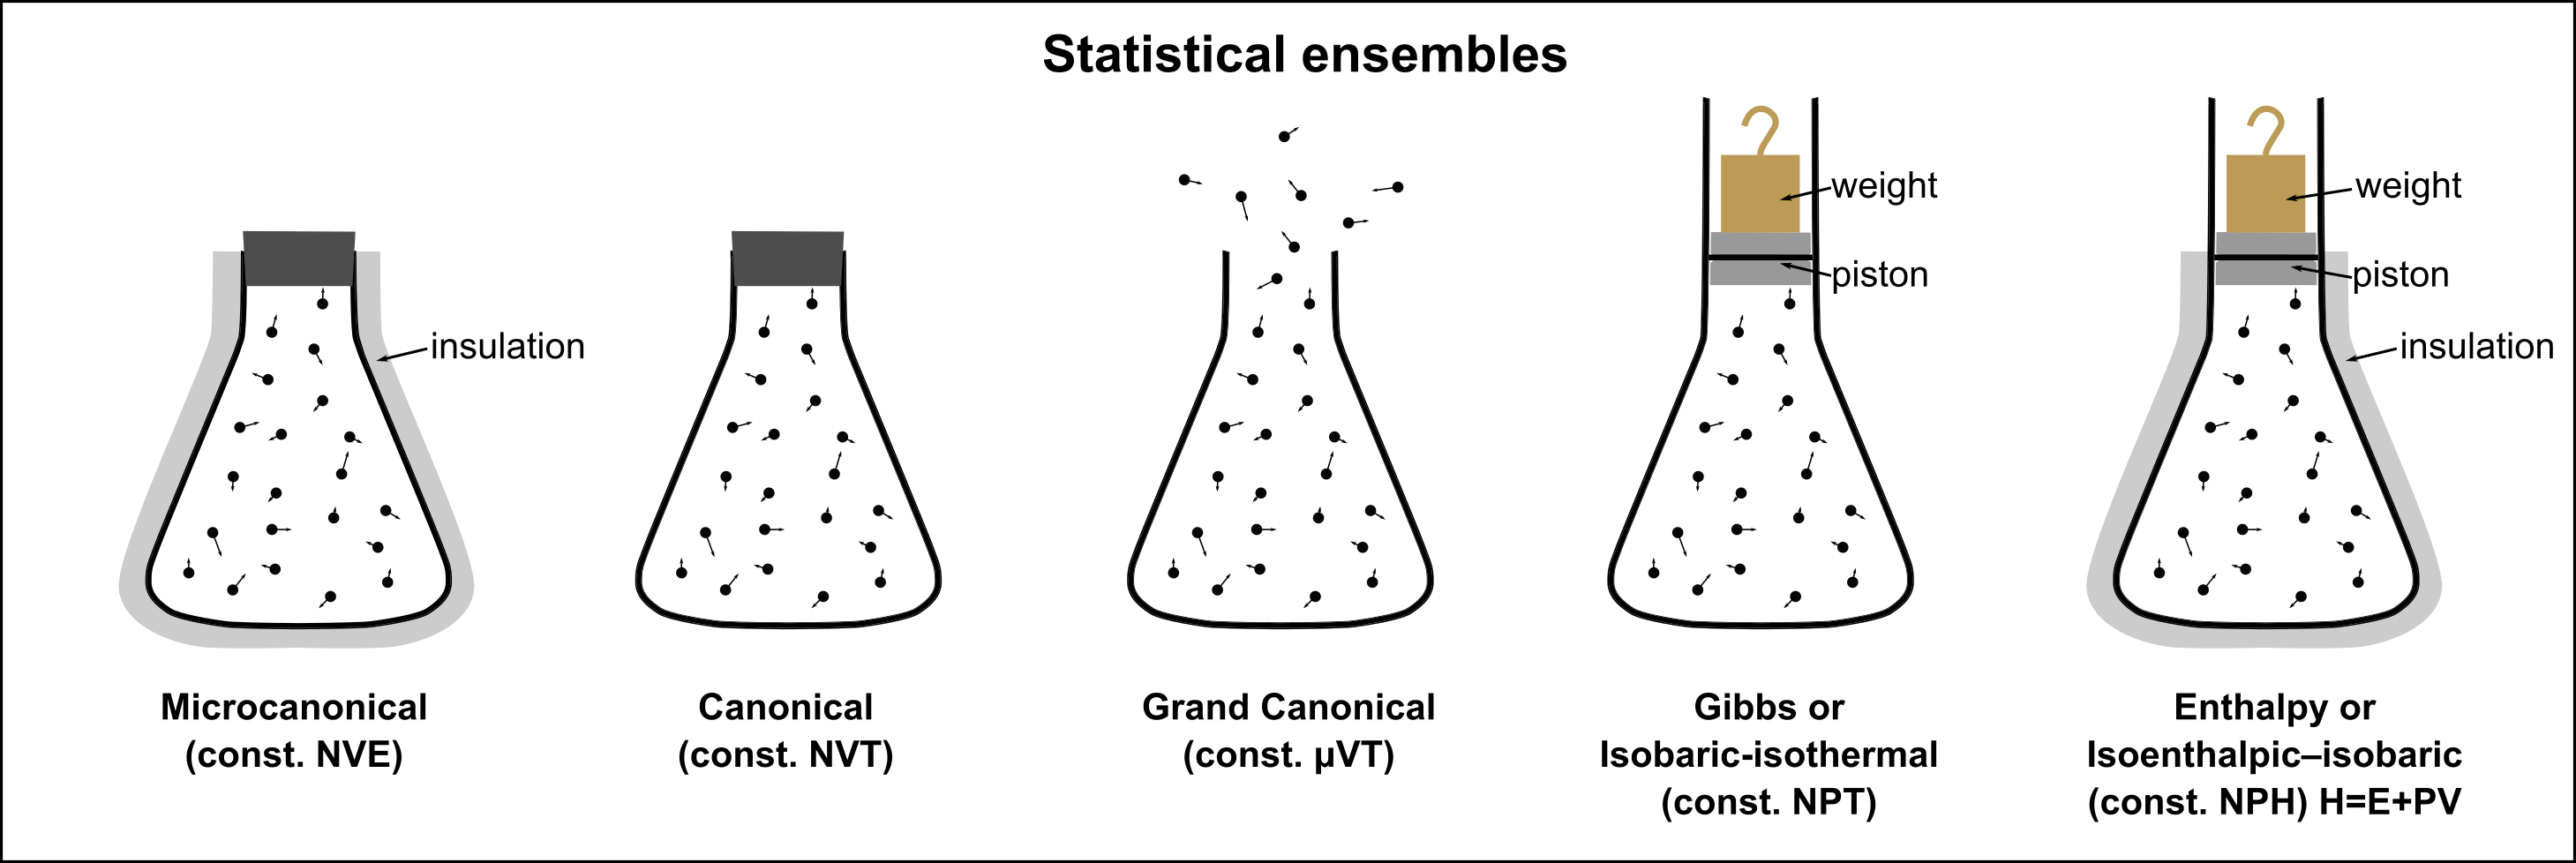
\includegraphics[height=1.60in,width=3.85in,viewport=0 0 1420 570,clip]{Figures/Statistical_Ensembles.png}
%%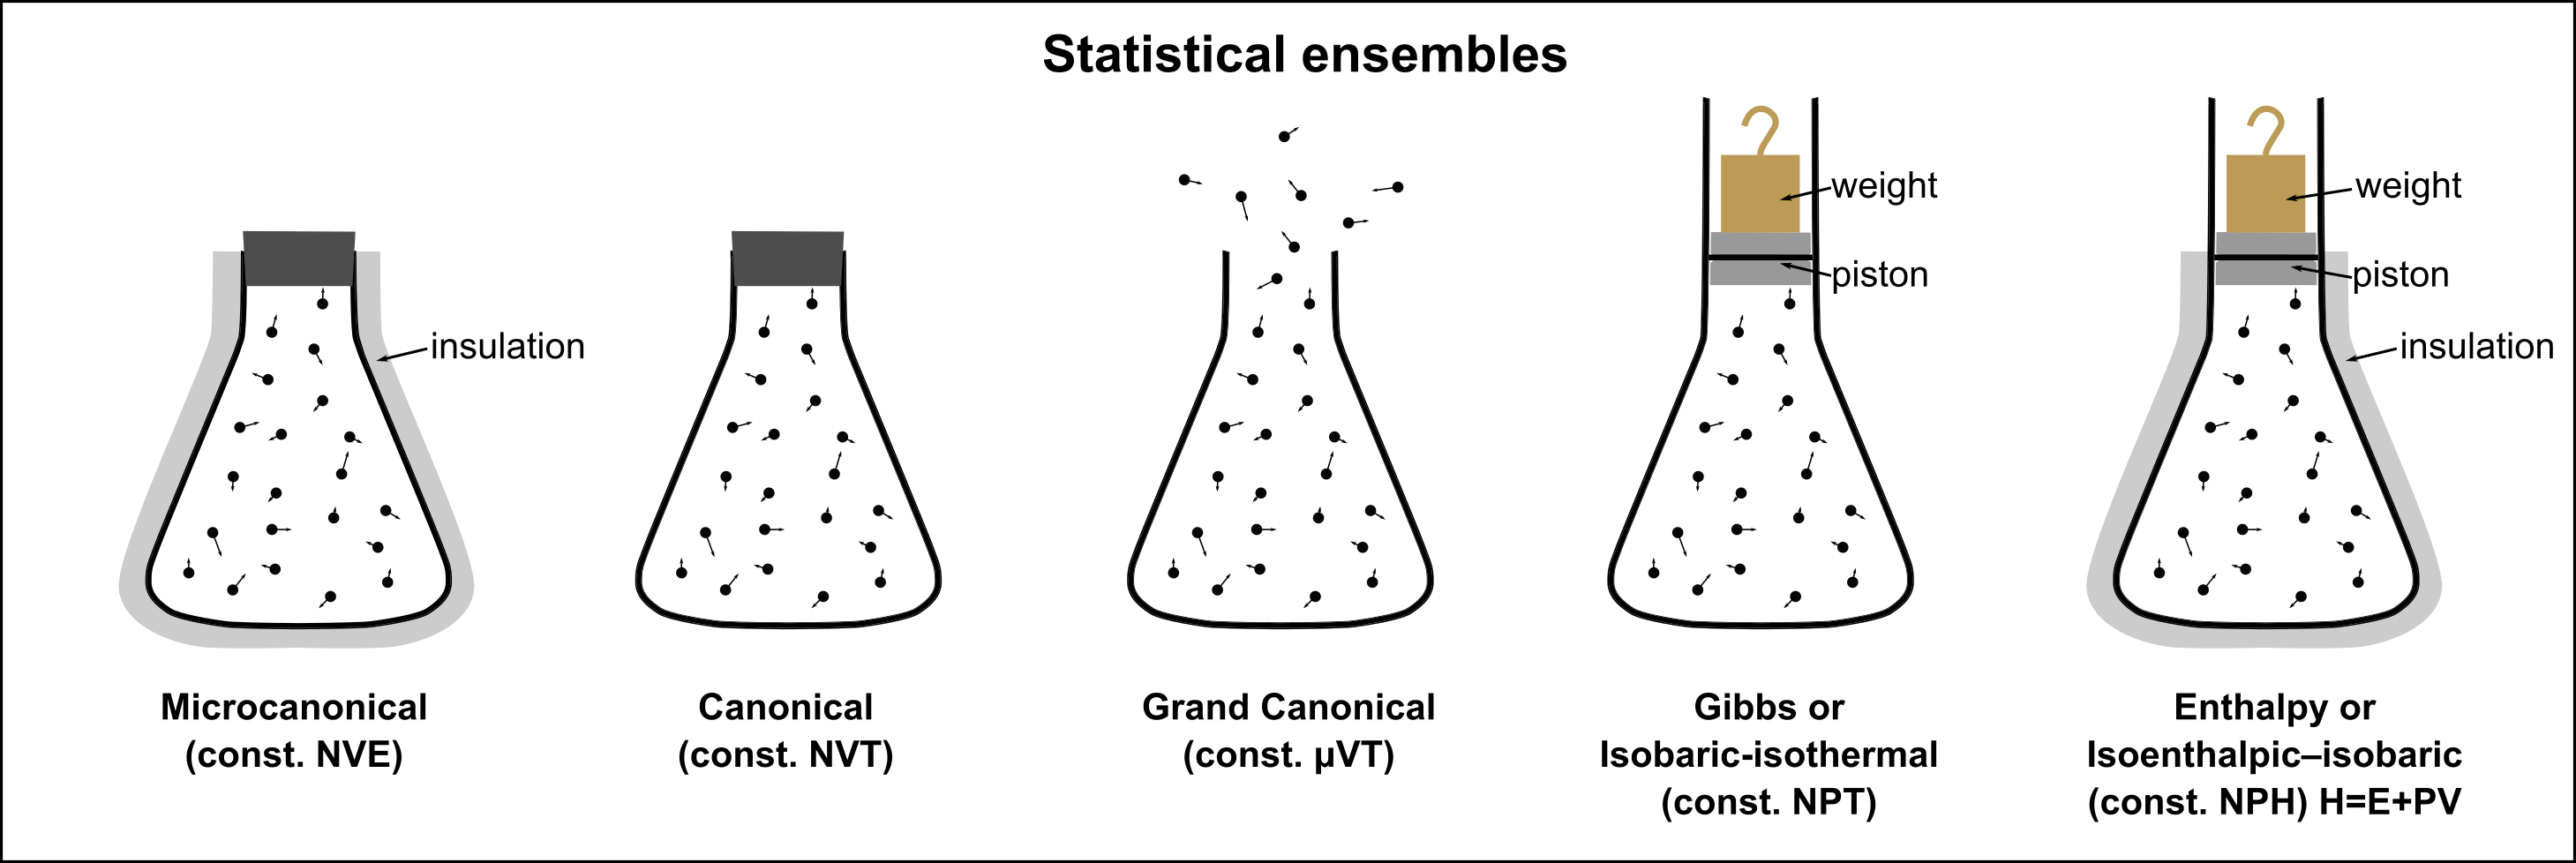
\includegraphics[height=1.30in,width=3.35in,viewport=0 0 1420 570,clip]{Figures/Statistical_Ensembles.png}
%%\caption{\tiny \textrm{The Statistical Ensembles.\footnote{\fontsize{3.5pt}{1.2pt}\selectfont{\textrm{canonical},汉译作“正则”,出自《楚辞\textperiodcentered 离骚》“皇揽揆余於初度兮,肇锡余以嘉名;~名余曰\textcolor{red}{正则}兮,字余曰灵均”,《楚辞章句》\upcite{Chucizhangju}:~“正,平也;~则,法也;~灵,神也;~均,调也。言正平可法则者,莫过于天;~养物均调者,莫过于地。高平曰原,故父伯庸名我为平以法天,字我为原以法地。言己上能安君,下能养民也。”,意思是说“正则”、“灵均”隐喻着某种意义,即平正是天的象征,原均是地的象征。因此正则的含义是“符合天道”,与\textrm{canonical}的意思\textrm{of, relating to, or forming a canon}意义一致。}}}}%(与文献\cite{EPJB33-47_2003}图1对比)
%\label{Statistical_Ensembles}
%\end{figure}
%}
%
%\frame
%{
%	\frametitle{第一原理分子动力学:~\textrm{CPMD}}
%	1985年\textrm{Car}和\textrm{Parrinello}在密度泛函理论基础上,将第一原理方法应用到分子动力学研究中,形成\textrm{Car-Parrinello Molecular dynamics~(CPMD)}
%	\begin{itemize}
%		\item 与\textrm{BOMD}不同,在\textrm{CPMD}中,电子自由度存在于经典\textrm{Lagrangian}中
%			\begin{displaymath}
%				\begin{aligned}
%					L_{\mathrm{CP}}(\{\psi_i\};~\mathbf{R},\dot{\mathbf{R}})=&\textcolor{blue}{\dfrac12\mu\sum_i\langle\dot{\psi}_i|\dot{\psi}_i\rangle}+\dfrac12\sum_{I=1}^NM_I\dot{\mathbf{R}}^2_I\\
%					-&\textcolor{red}{E}[\{\psi_i\};\mathbf{R}]\\
%					&+\sum_{ij}\Lambda_{ij}(\langle\psi_i|\psi_j\rangle-\delta_{ij})
%				\end{aligned}
%			\end{displaymath}
%			{\fontsize{6.2pt}{4.2pt}\selectfont{在经典\textrm{Lagrangian}中考虑电子自由度,人为地引入了傀电子质量参数$\mu$和傀轨道速度$\dot{\psi}_i$}}
%	\end{itemize}
%}
%
%\frame
%{
%	\frametitle{第一原理分子动力学:~\textrm{CPMD}}
%	\begin{itemize}
%		\item \textrm{CPMD}下的运动方程表示为
%			\begin{displaymath}
%				\begin{aligned}
%					M_I\ddot{\mathbf{R}}_I=&-\nabla_{\mathbf{R}_I}\bigg[E[\{\psi_i\};\mathbf{R}]\bigg|_{\{\langle\psi_i|\psi_j\rangle=\delta_{ij}\}}\bigg]\\
%					=&\textcolor{purple}{-\dfrac{\partial E}{\partial\mathbf{R}_I}}\textcolor{blue}{+\sum_{i,j}\Lambda_{ij}\dfrac{\partial}{\partial \mathbf{R}_I}\langle\psi_i|\psi_j\rangle}\\
%					\mu\ddot{\psi}_i(\vec r,t)=&-\dfrac{\delta E}{\delta\langle\psi_i|}+\sum_j\Lambda_{ij}|\psi_j\rangle\\
%					=&-\hat{H_{\mathrm{e}}}\langle\psi_j|+\sum_j\Lambda_{ij}|\psi_j\rangle
%				\end{aligned}
%			\end{displaymath}
%			{\fontsize{6.2pt}{4.2pt}\selectfont{$-\dfrac{\delta E}{\delta\langle\psi|}$表示经典力学框架下的电子受力,用来描述分子动力学范畴内电子自由度随原子核运动的情况 }}
%	\end{itemize}
%}

\frame
{
	\frametitle{\textrm{CPMD}计算的特点}
	\begin{itemize}
		\item 计算成本大大节约\\
			{\fontsize{8.2pt}{4.2pt}\selectfont{相比于\textrm{BOMD},\textrm{CPMD}无需在每个分子动力学时间步长执行电子自洽计算}}
		\item 计算时间步长不能太长\\
			{\fontsize{8.2pt}{4.2pt}\selectfont{绝热近似要求电子-核运动能量彼此分离,\textcolor{blue}{声子最高频率}$\omega_{\mathrm I}$必须远小于\textcolor{blue}{傀电子最低振动频率}$\omega_{\mathrm e}$
			\begin{displaymath}
				\omega_{\mathrm e}\propto\sqrt{\dfrac{\Delta E_{\mathrm{gap}}}{\mu}}
			\end{displaymath}
			$\Delta E_{\mathrm{gap}}$是\textrm{K-S}单粒子的带隙,许可最大时间步长$\Delta t_{\mathrm{max}}<1/\omega_{\mathrm{e}}$,大小主要由$\sqrt{\mu}$}}确定
		\item $\mu$物理上没有意义,但通过调节$\mu$可以平衡\textrm{AIMD}的效率和精度,一般选取$\mu$使得$\omega_{\mathrm{I}}<<\omega_{\mathrm{I}}$成立
		\item 对于金属/导体的\textrm{CPMD}计算,由于$\Delta E_{\mathrm{gap}}=0$,必须要求体系通过恒温条件平衡交换能或者泛函允许分数占据
		\end{itemize}
}

\subsection{含时密度泛函理论\rm{(TD-DFT)}}
\frame
{
	\frametitle{其它\textrm{AIMD}:~\textrm{PIMD}和\textrm{Ehrenfest~MD}}
	\begin{itemize}
		\item \textrm{Path Integral~MD~(PIMD)}\footnote{\fontsize{6.2pt}{4.2pt}\selectfont{基于量子统计的第一原理路径积分称为\textrm{Feynman}路径积分\textrm{(path integrals)}}}\\
			\textrm{PIMD}用量子力学计算电子和原子核运动,因此该方法比\textrm{BOMD}和\textrm{CPMD}方法精确,特别是对于含有轻元素体系——计算量也要大得多
		\item \textrm{Ehrenfest~MD}\\
			电子自由度通过求解含时\textrm{(Time-dependent)~Schr\"odinger}方程得到,当$\Delta t\rightarrow0$,自由度变化对应于电子的幺正传播\textrm{(unitary propagation)}\footnote{\fontsize{6.2pt}{4.2pt}\selectfont{\textrm{Ehrenfest~MD}的幺正变换确保波函数保持正交,但代价是积分时间步长必须极小,因此\textrm{Ehrenfest~MD}模拟时间尺度仅达\textrm{atto}$(10^{-18})$秒尺度}}
	\end{itemize}
	\textcolor{blue}{\textrm{CPMD}结合了\textrm{BOMD}与\textrm{Ehrenfest~MD}的优点}:
	\begin{itemize}
		\item 计算体系受力由总能对粒子位置的求导,并非求电子态的$\langle\Psi_0|\hat H_{\mathrm{e}}|\Psi_0\rangle$极小值
		\item 因为选择平面波基,$\vec F_{\mathrm{NSC}}$自然为0
	\end{itemize}
}

\frame
{\frametitle{含时\textrm{Schr\"odinger}方程}
对于核-电子体系,含时\textrm{Schr\"odinger}方程表示的动力学体系为
\begin{displaymath}
	\hat H\Psi(\vec r;\mathbf{R},t)=\mathrm{i}\hbar\dfrac{\partial}{\partial t}\Psi(\vec t;\mathbf{R},t)
\end{displaymath}
这里$\vec r=\{\vec r_1,\vec r_2,\cdots,\vec r_n\}$和$\mathbf{R}=\{\mathbf{R}_1,\mathbf{R}_2,\cdots,\mathbf{R}_I\}$分别表示电子与核的位置
\vskip 5pt
对于核-电子体系的动力学演化问题,同样需要考虑核-电子子体系和整体波函数的关系,对于电子体系,映射到无相互作用体系的思想就是含时\textrm{Kohn-Sham~(TDKS)}方程为核心的\textrm{TD-DFT}

\textrm{TD-DFT}分为两类
\begin{itemize}
	\item \textrm{LR~(Linear~Response)-TDDFT}:\\
		\textcolor{blue}{根据体系的电子结构得到体系的光谱信息}:~不产生体系的动力学演化信息
	\item \textrm{rt~(Real~Time)-TDDFT:}\\
		\textcolor{blue}{可用于演化体系,实现动力学模拟}
\end{itemize}
}

\frame
{
	\frametitle{第一原理分子动力学:~\rm{Enrenfest-MD}}
	\textrm{Ehrenfest}动力学要求体系总波函数$\Psi(\vec r;\mathbf{R},t)$随时间变化满足
	\begin{displaymath}
		\Psi(\vec r;\mathbf{R},t)=\psi(\vec r,t)\chi(\mathbf{R},t)\mathrm{exp}\bigg[\frac{\mathrm{i}}{\hbar}\int_{t_0}^t\mathrm{d}t^{\prime}E_{el}(t^{\prime})\bigg]
	\end{displaymath}
	指数部分称为波函数的相位项,写成
	\begin{displaymath}
		E_{el}(t)\iint\mathrm{d}\vec r\mathrm{d}\mathbf{R}~\psi^{\ast}(\vec r,t)\chi^{\ast}(\mathbf{R},t)H_{e,l}(\vec r;\mathbf{R})\psi(\vec r,t)\chi(\mathbf{R},t)
	\end{displaymath}
	注意:~电子波函数$\psi(\vec r,t)$不依赖于原子核的位置$\mathbf{R}$
	\vskip 3pt
	{\fontsize{6.2pt}{4.2pt}\selectfont{
电子-核体系的演化的含时自洽方程
\begin{displaymath}
	\begin{aligned}
		\mathrm{i}\hbar\frac{\partial\psi(\vec r,t)}{\partial t}=&-\frac{\hbar^2}2\sum_i\nabla_i^2\psi(\vec r,t)+\bigg[\mathrm{d}\mathbf{R}\chi^{\ast}(\mathbf{R},t)\hat{V}(\vec r;\mathbf{R})\chi(\mathbf{R},t)\bigg]\psi(\vec r,t)\\
		\mathrm{i}\hbar\frac{\partial\chi(\mathbf{R},t)}{\partial t}=&-\frac{\hbar^2}2\sum_{\gamma}\frac{\nabla_{\gamma}^2\chi(\mathbf{R},t)}{M_{\gamma}^{-1}}+\bigg[\mathrm{d}\vec r\psi^{\ast}(\vec {r},t)H_e(\vec r;\mathbf{R})\psi(\vec {r},t)\bigg]\chi(\vec R,t)
	\end{aligned}
\end{displaymath}
其中
\begin{displaymath}
	\hat{V}(\vec r;\mathbf{R})=-\sum_{\gamma}\frac{\hbar^2}{2M_{\gamma}}\nabla_{\gamma}^2+\sum_{i<j}\frac1{|\vec r_i-\vec r_j|}-\sum_{\gamma,i}\frac{Z_{\gamma}}{|\mathbf{R}_{\gamma}-\vec r_i|}+\sum_{\gamma<\zeta}\frac{Z_{\gamma}Z_{\zeta}}{|\mathbf{R}_{\gamma}|-|\mathbf{R}_{\zeta}|}
\end{displaymath} }}
}

\frame
{
	\frametitle{核运动方程}
	\textcolor{blue}{将原子核的波函数用极坐标形式表示
	\begin{displaymath}
		\chi(\mathbf{R},t)=A(\mathbf{R},t)\mathrm{exp}\bigg[\frac{\mathrm{i}}{\hbar}S(\mathbf{R},t)\bigg]
	\end{displaymath}}
	$\mathbf{A}(\mathbf{R},t)$是波函数的振幅,$\mathbf{S}(\mathbf{R},t)/\hbar$是相位
	\vskip 3pt
	代入原子核运动方程,在经典近似下(即取$\hbar\rightarrow0$),有
		\begin{displaymath}
			\frac{\partial S(\mathbf{R},t)}{\partial t}=-\frac12\sum_{\gamma}M_{\gamma}^{-1}(\nabla_{\gamma}S(\mathbf{R},t))^2\textcolor{magenta}{-\bigg[\int\mathrm{d}r\psi^{\ast}(\vec r,t)H_e(\vec r;\mathbf{R})\psi(\vec r,t)\bigg]}
		\end{displaymath}
		这是形如经典力学下的\textrm{Hamiloton-Jacobi~(HJ)}方程
\vskip 3pt
		方程表明核运动的量子体系在空间的径迹,可以用$\mathbf{S}(\mathbf{R},t)$在构象空间的偏微分方程描述
	}

\frame
{
	\frametitle{核运动方程}
	根据相空间中动量的定义$\mathbf{P}=\nabla_{\mathbf{R}}S(\mathbf{R})$,得到$\nabla_{\zeta}\mathbf{S}/M_{\zeta}=\mathbf{v}_{\zeta}$
	\vskip 3pt
	形如\textrm{HJ}的方程两侧对$\mathbf{R}_{\zeta}$取梯度$\nabla_{\zeta}$,并利用构象空间$(\mathbf{R},t)$中\textrm{Lagrangian}时间的全微分定义
		\begin{displaymath}
			\frac{\mathrm{d}}{\mathrm{d}t}\equiv\frac{\partial}{\partial t}+\sum_{\gamma}M_{\gamma}^{-1}\nabla_{\gamma}\mathbf{S}\cdot\nabla_{\gamma}
		\end{displaymath}
		可得到形如\textrm{Newton}方程的运动方程
		\begin{displaymath}
			\frac{\mathrm{d}\mathbf{P}_{\gamma}(t)}{\mathrm{d}t}=-\nabla_{\gamma}\bigg[\int\mathrm{d}\vec r\psi^{\ast}(\vec r,t)H_e(\vec r;\mathbf{R})\psi(\vec r,t)\bigg]
		\end{displaymath}
		或更简单的
		\begin{displaymath}
			M_{\gamma}\ddot{\mathbf{R}}_{\gamma}(t)=-\nabla_{\gamma}\bigg\langle H_e(\vec r;\mathbf{R}(t))\bigg\rangle
		\end{displaymath} 
}

\frame
{
	\frametitle{电子运动方程}
{\fontsize{8.2pt}{4.2pt}\selectfont{
	采用\textrm{Born-Oppenheimer}近似下,原子核波函数近似为
	\begin{displaymath}
		|\chi(\mathbf{R},t)|^2=\prod_{\gamma}\delta(\mathbf{R}_{\gamma}-\mathbf{R}_{\gamma}(t))
	\end{displaymath}
	电子体系的动力学演化方程
	\begin{displaymath}
		\mathrm{i}\hbar\frac{\partial\psi(\vec r;\mathbf{R(t)},t)}{\partial t}=H_e(\vec r;\mathbf{R}(t))\psi(\vec r;\mathbf{R}(t),t)
	\end{displaymath}
	\textrm{Hamiltonian}~$H_e(\vec r;\mathbf{R}(t))$和电子波函数$\psi(\vec r;\mathbf{R(t)},t)$参数化地依赖原子核位置$\mathbf{R}(t)$,使得电子运动与原子核运动耦合
	\vskip 3pt
	\textcolor{purple}{很多情况下,基于\textrm{DFT/TD-DFT}框架计算核-电子运动耦合方程中电子部分的贡献是合适的选择}
	\vskip 3pt
	\textcolor{blue}{根据\textrm{Runge-Gross}理论,体系电子密度演化函数为
	\begin{displaymath}
		\mathbf{A}[\rho]=\int_{t_0}^{t_1}\mathrm{d}t\bigg\langle\psi[\rho]\bigg|\mathrm{i}\hbar\frac{\partial}{\partial t}-\hat T-H_{ee}\bigg|\psi[\rho]\bigg\rangle
	\end{displaymath}}
	这里$H_{ee}$表示电子间相互作用,$\psi[\rho](t)$是由电荷密度确定的含时电子态波函数
}}
}

\frame
{
	\frametitle{含时\textrm{Kohn-Sham}方程}
{\fontsize{9.2pt}{4.2pt}\selectfont{
	电荷密度随时间演化函数用单电子\textrm{Kohn-Sham}波函数表示为
	\begin{displaymath}
		\begin{aligned}
			\mathbf{A}[\rho]=&\sum_i\int_{t_0}^{t_1}\mathrm{d}t\bigg\langle\phi_i(\vec r,t)\bigg|\mathrm{i}\hbar\frac{\partial}{\partial t}+\frac12\nabla^2\bigg|\phi_i(\vec r,t)\bigg\rangle\\
			&-H_{\mathrm{C}}[\rho(\vec r,t)]+\mathbf{A}_{\mathrm{XC}}[\rho(\vec r,t)]-\int\mathrm{d}\vec r\int_{t_0}^{t_1}\mathrm{d}t~v_{\mathrm{ext}}(\vec r,t)\rho(\vec r,t)
		\end{aligned}
	\end{displaymath}
	这里$H_{\mathrm{C}}(\vec r,t)$是\textrm{Hartree}能泛函
\vskip 3pt
在约束条件$\rho(\vec r,t)=\sum\limits_i|\phi_i(\vec r,t)|^2$下,通过变分法可得含时\textrm{Kohn-Sham~(TDKS)}方程
\begin{displaymath}
	\begin{aligned}
		\mathrm{i}\hbar\frac{\partial}{\partial t}\phi_i(\vec r,t)=&-\dfrac12\nabla^2\phi_i(\vec r,t)+v_i[\phi,\psi_0](\vec r,t)\phi_i(\vec r,t)\qquad i=1,2,3,\cdots,N\\
		v_i[\rho,\psi_0](\vec r,t)=&v_{\mathrm{ext}}(\vec r,t)+v_{\mathrm{H}}(\vec r,t)+\frac{\delta\mathbf{A}_{\mathrm{XC}}[\rho,\psi_0](\vec r,t)}{\delta\rho(\vec r,t)}
	\end{aligned}
\end{displaymath}
其中
\begin{displaymath}
	v_{\mathrm{ext}}(\vec r,t)=-\sum_{\gamma}\frac{Z_{\gamma}}{\vec r-\mathbf{R}_{\gamma}}+\delta_{\mathrm{app}}(\vec r,t)
\end{displaymath}
}}
}

\frame
{
	\frametitle{含时\textrm{Kohn-Sham}方程}
	对交换-相关项,考虑绝热近似\footnote{\fontsize{6.2pt}{4.2pt}\selectfont{绝热近似下,交换-相关泛函不随时间变化}}
\begin{displaymath}
	\mathbf{A}_{\mathrm{XC}}[\rho]=\int\mathrm{d}r\int_{t_0}^{t_1}\mathrm{d}t~\rho(\vec r,t)\epsilon_{\mathrm{XC}}[\rho(\vec r)]\bigg|_{\rho(\vec r)\leftarrow\rho(\vec r,t)}
\end{displaymath}

另外一种基于\textrm{DFT/TD-DFT}框架求解电子运动方程的方案,是用定态\textrm{Kohn-Sham}轨道$\{\phi_p^{\mathrm{opt}}(\vec r;\mathbf{R}(t))\}$来展开\textrm{TDKS}轨道,有
\begin{displaymath}
	\phi_i(\vec r,t)=\sum_{j}^{\infty}c_{ip}(t)\phi_p^{\mathrm{opt}}(\vec r;\mathbf{R}(t))
\end{displaymath}

\textrm{Ehrenfest-MD}的特点
\begin{itemize}
	\item \textrm{Ehrenfest-MD}是体系会在一个平均意义上的轨迹演化:\\
		可能不在任何一个确定的势能面上, 而在某两个甚至多个势能面加权的平均位置
	\item 不同状态的轨迹所对应的真实体系演化的物理图像相差很大:\\
		平均的\textrm{Ehrenfest}的轨迹的物理意义就会变得模糊
\end{itemize}
}

\frame
{
	\frametitle{\textrm{surface~hopping-MD}}
	总波函数的分解形式并不唯一,除了\textrm{Ehrenfest-MD}的形式,还可以按照\textrm{Born-Huang}的表达式来分解:
	\begin{displaymath}
		\Psi(\vec r;\mathbf{R},t)=\sum_i^{\infty}\chi_i(\mathbf{R},t)\psi_i(\vec r;\mathbf{R})
	\end{displaymath}
	这里$\{\psi(\vec r;\mathbf{R})\}$是一套完整的标准正交-归一的电子态波函数,是\textcolor{red}{定态}\textrm{Schr\"odinger}方程的解
	\begin{displaymath}
		H_e(\vec r,\mathbf{R})\psi_i(\vec r;\mathbf{R})=E_i^{e}(\mathbf{R})\psi_i(\vec r;\mathbf{R})
	\end{displaymath}
满足$\langle\psi_j|\psi_i\rangle=\delta_{ij}$
\vskip 5pt
因此,核-电子运动方程可以写成
\begin{displaymath}
	\mathrm{i}\hbar\frac{\partial}{\partial t}\chi_j(\mathbf{R},t)=\bigg[-\sum_{\gamma}\frac{\hbar^2}{2M_{\gamma}}\nabla_{\gamma}^2+E_j^{e}(\mathbf{R})\bigg]\chi_j(\mathbf{R},t)+\sum_i^{\infty}\mathbf{F}_{ji}\chi_i(\mathbf{R},t)
\end{displaymath}
}

\frame
{
	\frametitle{\textrm{surface~hopping-MD}}
其中
\begin{displaymath}
	\begin{aligned}
		\mathbf{F}_{ji}(\mathbf{R})=&\int\mathrm{d}\vec r~\psi_j^{\ast}(\vec r;\mathbf{R})\bigg[-\sum_{\gamma}\frac{\hbar^2}{2M_{\gamma}}\nabla_{\gamma}^2\bigg]\psi_i(\vec r;\mathbf{R})\\
		&+\sum_{\gamma}\frac1{M_{\gamma}}\bigg\{\mathrm{d}\vec r\psi_j^{\ast}(\vec r;\mathbf{R})[-\mathrm{i}\hbar\nabla_{\gamma}]\psi_i(\vec r;\mathbf{R})\bigg\}\times[-\mathrm{i}\hbar\nabla_{\gamma}]
	\end{aligned}
\end{displaymath}
是非绝热耦合\textrm{(nonadiabatic coupling, NACs)}的贡献:
\begin{itemize}
	\item 第一项来自于核动能算符
	\item 第二项来自于动量算符
\end{itemize}
{\fontsize{8.2pt}{4.2pt}\selectfont{一般情况下, 当非对角元有贡献时, 可理解为\textcolor{red}{原子核的运动引起不同电子态之间的耦合}(\textcolor{blue}{同时会伴随声子的吸收和释放})}}

$\mathbf{F}_{ji}(\mathbf{R})$的表达式中还包含从电子态$i$到$j$的贡献,这两个电子态分别是能量$E_i^{e}(\mathbf{R})$和$E_j^{e}(\mathbf{R})$的电子本征态。这是该方法称为\textrm{surface~hopping-MD}的原因
}

\frame
{
	\frametitle{\textrm{BOMD}}
	在\textrm{Born-Oppenheimer}近似下,$\mathbf{F}_{ji}(\mathbf{R})$仅对角项有贡献
	\begin{displaymath}
		\mathbf{F}_{jj}(\mathbf{R})=\int\mathrm{d}\vec r~\psi_j^{\ast}(\vec r;\mathbf{R})\bigg[-\sum_{\gamma}\frac{\hbar^2}{2M_{\gamma}}\nabla_{\gamma}^2\bigg]\psi_i(\vec r;\mathbf{R})
	\end{displaymath}
	因此核与电子运动完全解耦,核在电子贡献的势能面$E_j^{e}(\mathbf{R})$上,遵从单粒子运动方程
	\begin{displaymath}
		\mathrm{i}\hbar\frac{\partial}{\partial t}\chi_j(\mathbf{R},t)=\bigg[-\sum_{\gamma}\frac{\hbar^2}{2M_{\gamma}\nabla_{\gamma}^2+E_j^{e}(\mathbf{R})+\mathbf{F}_{jj}(\mathbf{R})}\bigg]\chi_j(\mathbf{R},t)
	\end{displaymath}
	\textcolor{blue}{$\mathbf{F}_{jj}(\mathbf{R})$一般比较小,可以忽略}
\vskip 5pt
与\textrm{Ehrenfest-MD}中类似,\textcolor{blue}{如果核波函数表示为极坐标形式:
\begin{displaymath}
	\chi_j(\mathbf{R},t)=\mathbf{A}_j(\mathbf{R},t)\mathrm{exp}\bigg[\frac{\mathrm{i}}{\hbar}\mathbf{S}_j(\mathbf{R},t)\bigg]
\end{displaymath}}
}

\frame
{
	\frametitle{\textrm{BOMD}的核运动方程}
{\fontsize{7.2pt}{4.2pt}\selectfont{
核运动方程为
\begin{displaymath}
	\begin{aligned}
		\frac{\partial\mathbf{S}_j(\mathbf{R},t)}{\partial t}=&\frac{\hbar^2}2\sum_{\gamma}M_{\gamma}^{-1}\frac{\nabla_{\gamma}^2\mathbf{A}_j(\mathbf{R},t)}{\mathbf{A}_j(\mathbf{R},t)}-\frac12\sum_{\gamma}M_{\gamma}^{-1}(\nabla_{\gamma}\mathbf{S}_j(\mathbf{R},t))^2-E_j^{e}(\mathbf{R})\\
		\frac{\partial\mathbf{A}_j(\mathbf{R},t)}{\partial t}=&-\sum_{\gamma}M_{\gamma}^{-1}\nabla_{\gamma}\mathbf{A}_j(\mathbf{R},t)\cdot\nabla_{\gamma}\mathbf{S}_j(\mathbf{R},t)-\frac12\sum_{\gamma}M_{\gamma}^{-1}\mathbf{A}_j(\mathbf{R},t)\nabla_{\gamma}^2\mathbf{S}(\mathbf{R},t)
	\end{aligned}
\end{displaymath}
经典近似下,取$\hbar\rightarrow0$,则有
\begin{displaymath}
	\frac{\partial\mathbf{S}_j(\mathbf{R},t)}{\partial t}=-\frac12\sum_{\gamma}M_{\gamma}^{-1}(\nabla_{\gamma}\mathbf{S}_j(\mathbf{R},t))^2-E_j^{e}(\mathbf{R})
\end{displaymath}
取$\nabla_{\gamma}\mathbf{S}_j|_{(\mathbf{R}(t)}=\mathbf{P}_j^{\gamma}(t)$
得到经典的原子核在电子态$j$中演化的运动方程
\begin{displaymath}
	\begin{aligned}
		M_{\gamma}\ddot{\mathbf{R}}_j^{\gamma}(t)=&-\nabla_{\gamma}E_j^{e}(\mathbf{R}(t))\\
		=&-\mathop{\nabla_{\gamma}}\limits_{\mathrm{min}\psi_j}\big\langle\psi_{\gamma}|H_e(r,\mathbf{R(t)})|\psi_j\big\rangle
	\end{aligned}
\end{displaymath}
}}
}

\frame
{
	\frametitle{非绝热\textrm{Bohmian}动力学\textrm{(NABMD)}}
	针对激发态,不能简单地采取\textrm{Born-Oppenheimer}近似
\vskip 5pt	
{\fontsize{8.2pt}{4.2pt}\selectfont{
	核-电子耦合运动方程应写成
	\begin{displaymath}
		\begin{aligned}
			\mathrm{i}\hbar\frac{\partial\chi_j(\mathbf{R},t)}{\partial t}=&-\sum_{\gamma}\frac{\hbar^2}{2M_{\gamma}}\nabla_{\gamma}^2\chi_j(\mathbf{R},t)+E_j^{e}(\mathbf{R})\chi_j(\mathbf{R},t)\\
			&+\sum_{\gamma i}\frac{\hbar^2}{2M_{\gamma}}\mathbf{D}_{ji}^{\gamma}\chi_i(\mathbf{R},t)-\sum_{\gamma,i\neq j}\mathbf{d}_{ji}^{\gamma}(\mathbf{R})\cdot\nabla_{\gamma}\chi_i(\mathbf{R},t)
		\end{aligned}
	\end{displaymath}
	这里
	\begin{displaymath}
		\mathbf{d}_{ji}^{\gamma}(\mathbf{R})=\int\mathrm{d}\vec r~\psi^{\ast}_j(\vec r;\mathbf{R})\nabla_{\gamma}\psi_i(\vec r;\mathbf{R})
	\end{displaymath}
	是一阶非绝热耦合系数
	\begin{displaymath}
		\mathbf{D}_{ji}^{\gamma}(\mathbf{R})=\int\mathrm{d}\vec r~\psi^{\ast}_j(\vec r;\mathbf{R})\nabla_{\gamma}^2\psi_i(\vec r;\mathbf{R})
	\end{displaymath}
	是二阶非绝热耦合系数\\
因此核运动波函数的演化方程为
}}
}

\frame
{
	\frametitle{非绝热\textrm{Bohmian}动力学\textrm{(NABMD)}}
{\fontsize{6.2pt}{4.2pt}\selectfont{
	根据核波函数的演化形式,可有核运动的方程
	\begin{displaymath}
		\begin{aligned}
			\frac{\partial\mathbf{S}_j(\mathbf{R},t)}{\partial t}=&\sum_{\gamma}\frac1{2M_{\gamma}}(\nabla_{\gamma}\mathbf{S}_j(\mathbf{R},t))^2\textcolor{red}{+E_j^{e}(\mathbf{R})}\textcolor{blue}{-\sum_{\gamma}\frac{\hbar^2}{2M_{\gamma}}\frac{\nabla_{\gamma}^2\mathbf{A}_j(\mathbf{R},t)}{\mathbf{A}_j(\mathbf{R},t)}}\\
			&\textcolor{purple}{+\sum_{\gamma i}\frac{\hbar^2}{2M_{\gamma}}\mathbf{D}_{ji}^{\gamma}(\mathbf{R})\frac{\nabla_{\gamma}^2\mathbf{A}_j(\mathbf{R},t)}{\mathbf{A}_j(\mathbf{R},t)}\Re\bigg[\mathrm{e}^{\mathrm{i}\phi_{ij}(\mathbf{R},t)}\bigg]}\\
			&\textcolor{purple}{-\sum_{\gamma,i\neq j}\frac{\hbar^2}{M_{\gamma}}\cdot\frac{\nabla_{\gamma}\mathbf{A}_i(\mathbf{R},t)}{\mathbf{A_j(\mathbf{R},t)}}\Re\bigg[\mathrm{e}^{\mathrm{i}\phi_{ij}(\mathbf{R},t)}\bigg]}\\
			&\textcolor{purple}{+\sum_{\gamma,i\neq j}\frac{\hbar}{M_{\gamma}}\frac{\mathbf{A}_i(\mathbf{R},t)}{\mathbf{A}_j(\mathbf{R},t)}\mathbf{d}_{ji}^{\gamma}(\mathbf{R})\cdot\nabla_{\gamma}\mathbf{S}_i(\mathbf{R},t)\times\Im\bigg[\mathrm{e}^{\mathrm{i}\phi_{ij}(\mathbf{R},t)}\bigg]}\\
			\frac{\partial\mathbf{A}_j(\mathbf{R},t)}{\partial t}=&-\sum_{\gamma}\frac{\hbar}{M_{\gamma}}\nabla_{\gamma}\mathbf{A}_j(\mathbf{R},t)\cdot\nabla_{\gamma}\mathbf{S}_j(\mathbf{R},t)\textcolor{blue}{-\sum_{\gamma}\frac{\hbar}{2M_{\gamma}}\mathbf{A}_j(\mathbf{R},t)\nabla_{\gamma}^2\mathbf{S}(\mathbf{R},t)}\\
			&\textcolor{purple}{+\sum_{\gamma i}\frac{\hbar^2}{2M_{\gamma}}\mathbf{D}_{ji}^{\gamma}(\mathbf{R})\mathbf{A}_i(\mathrm{R},t)\Im\bigg[\mathrm{e}^{\mathrm{i}\phi_{ij}(\mathbf{R},t)}\bigg]}\\
			&\textcolor{purple}{-\sum_{\gamma,i\neq j}\frac{\hbar^2}{M_{\gamma}}\mathbf{d}_{ji}^{\gamma}(\mathbf{R})\cdot\nabla_{\gamma}\mathbf{A}_i(\mathbf{R},t)\Im\bigg[\mathrm{e}^{\mathrm{i}\phi_{ij}(\mathbf{R},t)}\bigg]}\\
			&\textcolor{purple}{-\sum_{\gamma,i\neq j}\frac{\hbar}{M_{\gamma}}\mathbf{A}_i(\mathbf{R},t)\mathbf{d}_{ji}^{\gamma}(\mathbf{R})\cdot\nabla_{\gamma}\mathbf{S}_i(\mathbf{R},t)\times\Re\bigg[\mathrm{e}^{\mathrm{i}\phi_{ij}(\mathbf{R},t)}\bigg]}
		\end{aligned}
	\end{displaymath}
	其中$\phi_{ij}(\mathbf{R},t)=\frac1{\hbar}\big(\mathbf{S}_i(\mathbf{R},t)-\mathbf{S}_j(\mathbf{R},t)\big)$
}}
}

\frame
{
	\frametitle{非绝热\textrm{Bohmian}动力学\textrm{(NABMD)}}
	同样类似地,对相位$\mathbf{S}(\mathbf{R},t)$,引入动量定义$\nabla_{\beta}\mathbf{S}_j(\mathbf{R},t)|_{\mathbf{R(t)}}=\mathbf{P}_j^{\beta}(t)$,核波函数的相位演化方程可以写成
	\begin{displaymath}
		M_{\beta}\frac{\mathrm{d}^2\mathbf{R}_{\beta}(t)}{(\mathrm{d}t^j)^2}=-\nabla_{\beta}\bigg[E_j^{e}(\mathbf{R}(t))+\textcolor{blue}{\mathbf{Q}_j(\mathbf{R}(t),t)}+\textcolor{purple}{\sum_i\mathbf{D}_{ji}(\mathbf{R}(t),t)}\bigg]
	\end{displaymath}
	该方程描述了\textcolor{blue}{群体变量$\mathbf{R}(t)$}构成的流体,其分量$\mathbf{R}_{\beta}$随时间的演化\\
	其中全微分定义为
	\begin{displaymath}
		\mathrm{d}/\mathrm{d}t^j=\partial/\partial t+\sum_{\gamma}\nabla_{\gamma}\mathbf{S}_j(\mathbf{R},t)/M_{\gamma}\cdot\nabla_{\gamma}
	\end{displaymath}
	\begin{itemize}
		\item \textcolor{blue}{$\mathbf{Q}_j(\mathbf{R}(t),t)$}是量子势\\
			它描述了单电子态下的量子效应,引入非局域属性
		\item \textcolor{purple}{$\sum\limits_{ji}\mathbf{D}_{ji}(\mathbf{R}(t),t)$}是非绝热量子势\\
			它包含一阶和二阶非绝热耦合系数,使得电子态之间发生迁移
	\end{itemize}
}

\frame
{
	\frametitle{\textrm{TSH}方法}
{\fontsize{8.2pt}{4.2pt}\selectfont{
	\textrm{Tully}等将上述精确表达式保留到$\mathcal{O}(\hbar)$到一阶则有
	\begin{displaymath}
		\begin{aligned}
			\frac{\partial\mathbf{S}_j(\mathbf{R},t)}{\partial t}=&\sum_{\gamma}\frac1{2M_{\gamma}}(\nabla_{\gamma}\mathbf{S}_j(\mathbf{R},t))^2+E_j^{e}(\mathbf{R})\\
			&\textcolor{purple}{+\sum_{\gamma,i\neq j}\frac{\hbar}{M_{\gamma}}\frac{\mathbf{A}_i(\mathbf{R},t)}{\mathbf{A}_j(\mathbf{R},t)}\mathbf{d}_{ji}^{\gamma}(\mathbf{R})\cdot\nabla_{\gamma}\mathbf{S}_i(\mathbf{R},t)\times\Im\bigg[\mathrm{e}^{\mathrm{i}\phi_{ij}(\mathbf{R},t)}\bigg]}\\
			\frac{\partial\mathbf{A}_j(\mathbf{R},t)}{\partial t}=&-\sum_{\gamma}\frac{\hbar}{M_{\gamma}}\nabla_{\gamma}\mathbf{A}_j(\mathbf{R},t)\cdot\nabla_{\gamma}\mathbf{S}_j(\mathbf{R},t)\\
			&-\sum_{\gamma}\frac{\hbar}{2M_{\gamma}}\mathbf{A}_j(\mathbf{R},t)\nabla_{\gamma}^2\mathbf{S}_j(\mathbf{R},t)\\
			&\textcolor{purple}{-\sum_{\gamma,i\neq j}\frac{\hbar}{M_{\gamma}}\mathbf{A}_i(\mathbf{R},t)\mathbf{d}_{ji}^{\gamma}(\mathbf{R})\cdot\nabla_{\gamma}\mathbf{S}_i(\mathbf{R},t)\times\Re\bigg[\mathrm{e}^{\mathrm{i}\phi_{ij}(\mathbf{R},t)}\bigg]}
		\end{aligned}
	\end{displaymath}
	被称为\textrm{Trajectory Surface-Hopping~(TSH)}方法
	\vskip 5pt
	\textrm{TSH}方法是介于完全绝热近似和完全精确的\textrm{NABDY}方法之间的处理方案
}}
}

\frame
{
	\frametitle{\textrm{TSH}方法:~准经典部分}
{\fontsize{8.2pt}{4.2pt}\selectfont{
	\textcolor{blue}{核体系波函数演化过程的准经典部分}构成构象空间$(\mathbf{R},t)$的轨迹\textrm{(trajectory)}

	在\textrm{TSH}方法中,$\mathbf{S}_j(\mathbf{R},t)$可以视为作用量,因此体系的轨迹由最小作用原理确定,即$\mathbf{S}(\mathbf{R},\mathbf{P},t)=0$。与经典力学的相空间描述类似,假设不同初始态对应的粒子演化轨迹彼此独立(轨迹独立假设,\textrm{ITA}),\textcolor{red}{核波函数的概率密度(振幅的平方)可用穿过单位空间微元的轨迹数量的比例来计算},即
	\begin{displaymath}
		\bigg(\mathbf{A}_j^{\mathrm{CL}}(\mathbf{R}(t),t)\bigg)^2=\frac{N_j(\mathbf{R}(t),\mathrm{d}V,t)}{N_t}\frac1{\mathrm{d}V}
	\end{displaymath}
	其中$N_j(\mathbf{R}(t),\mathrm{d}V,t)$表示穿过体积微元$\mathrm{d}V\equiv\mathrm{d}^{3N_n}\mathbf{R}$的径迹总数
	\vskip 3pt
	\textcolor{blue}{注意:~这里给出的核经典轨迹由与非绝热耦合系数$\mathbf{d}_{ji}^{\gamma}(\mathbf{R}(t))$无关部分确定}
\vskip 3pt
	因此可有
	\begin{displaymath}
		\begin{aligned}
			-\frac{\partial\mathbf{S}_j^{\mathrm{CL}}(\mathbf{R},t)}{\partial t}=&\sum_{\gamma}\frac1{2M_{\gamma}}(\nabla_{\gamma}\mathbf{S}_j(\mathbf{R},t))^2+E_j^{e}(\mathbf{R})\\
			\frac{\partial\mathbf{A}_j^{\mathrm{CL}}(\mathbf{R},t)}{\partial t}=&-\sum_{\gamma}\frac1{M_{\gamma}}\nabla_{\gamma}\mathbf{A}_j^{\mathrm{CL}}(\mathbf{R},t)\cdot\nabla_{\gamma}\mathbf{S}_j^{\mathrm{CL}}(\mathbf{R},t)\\
			&-\sum_{\gamma}\frac1{2M_{\gamma}}\mathbf{A}_j^{\mathrm{CL}}(\mathbf{R},t)\nabla_{\gamma}^2\mathbf{S}_j^{\mathrm{CL}}(\mathbf{R},t)
		\end{aligned}
	\end{displaymath}
}}
}

\frame
{
	\frametitle{\textrm{TSH}方法:~准经典部分}
	上述方程确定了核运动的相位准经典部分$\mathbf{S}_j^{\mathrm{CL}}(\mathbf{R},t)$和振幅的准经典部分$\mathbf{A}_j^{\mathrm{CL}}(\mathbf{R},t)$的演化过程,不难看出其与\textrm{Newton}运动方程等价
\begin{displaymath}
	\frac{\mathrm{d}\mathbf{P}_j^{\beta}(t)}{\mathrm{d}t^j}=-\nabla_{\beta}E_j^{e}(\mathbf{R}(t))
\end{displaymath}
其中
\begin{displaymath}
	\mathbf{P}_j(t)=\nabla\mathbf{S}_j^{\mathrm{CL}}(\mathrm{R},t)|_{\mathbf{R}(t)}
\end{displaymath}

\textcolor{red}{在此基础上,考虑非绝热耦合项的贡献,原子核将沿经典轨迹运动时感受到量子效应引起的附加力}

这种附加作用会使得经典概率密度$\bigg(A_j^{\mathrm{CL}}(\mathbf{R}(t),t)\bigg)^2$在电子态间传播(即体系可以在不同势能面之间跃迁)
}

\frame
{
	\frametitle{\textrm{TSH}方法:~量子部分}
{\fontsize{8.2pt}{4.2pt}\selectfont{
	定义核运动的量子相位$\mathbf{S}_i^{\mathrm{QM}}(\mathbf{R}(t),t)$和量子振幅$\mathbf{A}_j^{\mathrm{QM}}(\mathbf{R}(t),t)$,其演化方程由非决人耦合项贡献确定,即
	\begin{displaymath}
		\begin{aligned}
			-\frac{\partial\mathbf{S}_j^{\mathrm{QM}}(\mathbf{R},t)}{\partial t}=&E_j^{e}(\mathbf{R})\textcolor{purple}{+\sum_{\gamma,i\neq j}\frac{\hbar}{M_{\gamma}}\frac{\mathbf{A}_i^{\mathrm{QM}}(\mathbf{R},t)}{\mathbf{A}_j^{\mathrm{QM}}(\mathbf{R},t)}}\\
			&\textcolor{purple}{\times\mathbf{d}_{ji}^{\gamma}(\mathbf{R})\cdot\dot{\mathbf{R}}_{\gamma}(t)\Im\bigg[\mathrm{e}^{\mathrm{i}\phi_{ij}^{\mathrm{QM}}(\mathbf{R},t)}\bigg]}\\
			\frac{\partial\mathbf{A}_j^{\mathrm{QM}}(\mathbf{R},t)}{\partial t}=&\textcolor{purple}{-\sum_{\gamma,i\neq j}\frac{\hbar}{M_{\gamma}}\mathbf{A}_i^{\mathrm{QM}}(\mathbf{R},t)}\\
			&\textcolor{purple}{\times\mathbf{d}_{ji}^{\gamma}(\mathbf{R})\cdot\dot{\mathbf{R}}_{\gamma}(\mathbf{R}(t))\Re\bigg[\mathrm{e}^{\mathrm{i}\phi_{ij}^{\mathrm{QM}}(\mathbf{R},t)}\bigg]}
		\end{aligned}
	\end{displaymath}
	其中
	\begin{displaymath}
		\phi_{ij}^{\mathrm{QM}}(\mathbf{R(t)},t)=\frac1{\hbar}\bigg(\mathbf{S}_i^{\mathrm{QM}}(\mathbf{R}(t),t)-\mathbf{S}_j^{\mathrm{QM}}(\mathbf{R}(t),t)\bigg)
	\end{displaymath}
	这是极坐标形式下的\textrm{Tully-TSH}方程
}}
}

\frame
{
	\frametitle{\textrm{TSH}方法:~量子部分}
	定义
\begin{displaymath}
	C_j(\mathbf{R}(t),t)=\mathbf{A}_j^{\mathrm{QM}}(\mathbf{R}(t),t)\mathrm{exp}\bigg[\frac{\mathrm{i}}{\hbar}\mathbf{S}_j^{\mathrm{QM}}(\mathbf{R}(t),t)\bigg]
\end{displaymath}
则有
\begin{displaymath}
	\begin{aligned}
		\mathrm{i}\hbar\frac{\partial C_j(\mathrm{R}(t),t)}{\partial t}=&C_j(\mathbf{R}(t),t)E_n^{e}(\mathbf{R}(t))\\
		&-\mathrm{i}\hbar\sum_i(\mathbf{d_{ji}}(\mathbf{R}(t)))\cdot\dot{\mathbf{R}}(t)C_i(\mathbf{R}(t,t))
	\end{aligned}
\end{displaymath}
严格说,量子相位$\mathbf{S}_j^{\mathrm{QM}(\mathbf{R}(t),t)}$,量子振幅$\mathbf{A}_j^{\mathrm{QM}(\mathbf{R}(t),t)}$ 和$C_j(\mathbf{R}(t,t))$都不是经典构象空间$(\mathbf{R},t)$的描述量,然而它们依然可以近似与经典轨迹相对应

在\textrm{TSH}动力学中,准经典部分和量子部分的方程同时求解,并认为只要统计轨迹足够多,将有
\begin{displaymath}
	\bigg(\mathbf{A}_j^{\mathrm{CL}}(\mathbf{R},t),t\bigg)^2=\bigg(\mathbf{A}_j^{\mathrm{QM}}(\mathbf{R},t),t\bigg)^2
\end{displaymath}
}

\frame
{
	\frametitle{\textrm{TSH}方法:~跃迁几率}
	\textrm{Tully}给出$t$时刻统计随后$\Delta t$时间内由$j$向$i$跃迁几率的表达式
			\begin{displaymath}
				p_{i\leftarrow j}^{[\alpha]}(t,t+\Delta t)=-2\int_t^{t+\Delta t}\mathrm{d}\tau\frac{\Re\bigg[C_i^{[\alpha]}(\tau)C_j^{[\alpha]\ast}(\tau)\dot{\mathbf{R}}(\tau)\cdot\mathbf{d}_{ij}(\mathbf{R}(\tau))\bigg]}{C_j^{[\alpha]}(\tau)C_j^{[\alpha]\ast}(\tau)}
			\end{displaymath}
			实际计算中可采用\textrm{Monte-Carlo}的思想来确定态间跃迁,比如生成随机数$\zeta\in[0,1]$,只有当满足
			\begin{displaymath}
				\sum_{k\leqslant i-1}p_{k\leftarrow j}^{[\alpha]}<\zeta<\sum_{k\leqslant i}p_{k\leftarrow j}^{[\alpha]}
			\end{displaymath}
			会认为体系中出现$j$向$i(i\neq j)$的跃迁
			\vskip 5pt
			\textrm{TSH}是严格的\textrm{NABDY}的基础上引入假设:
	\begin{itemize}
		\item 每个电子态$j$下, 核动力学可以分为经典分量和量子分量%分别由对应的相位和振幅描述
		\item \textrm{Tully}引入跃迁几率$P_{i\leftarrow j}^{[\alpha]}$,
			使得经典振幅和量子振幅的平方一致
	\end{itemize}
}
\frame
{
	\frametitle{平衡态统计基础}
	系综(\textrm{Ensembles})是在一定的宏观条件下,由大量微观粒子组成的性质和结构完全相同的、处于各种运动状态的、各自独立的系统整体的集合。简言之,系综是给定宏观条件下,所有微观状态的集合。
%	应用\textrm{Verlet}算法,完成单粒子运动的数值积分,可以得到动力学体系的\textrm{Hamiltonian}对应的能量,进而应用统计力学的统计系综,获得宏观体系的物理量
	\vskip 3pt
	\textcolor{blue}{等概率原理}\textrm{(Principle of equal weights)}:\\
	一个热力学体系有相同的概率到达每个可能经历的微观态。\\
	等概率原理导出\textrm{Boltzmann}分布
	\begin{displaymath}
		P_j=\dfrac{\mathrm{e}^{-\beta\varepsilon_j}}Q
	\end{displaymath}
	这里$Q$称为配分函数\textrm{(partition function)}
	\begin{displaymath}
		\begin{aligned}
			Q=&\sum_i\mathrm{e}^{(-\beta\varepsilon_i)}\\
			\beta=&1/k_{\mathrm{B}}T
		\end{aligned}
	\end{displaymath}
	物理量的系综平均
	\begin{displaymath}
		\langle A\rangle=\sum_jA_j\mathrm{e}^{(-\beta\varepsilon_j)}/Q
	\end{displaymath}
}

\frame
{
	\frametitle{常用统计系综}
	{\fontsize{8.2pt}{4.2pt}\selectfont{应用\textrm{Verlet}算法,完成单粒子运动的数值积分,可以得到动力学体系的\textrm{Hamiltonian}对应的能量,基于统计系综,可获得体系的宏观物理量}}
\begin{figure}[h!]
\centering
\vspace*{-0.05in}
%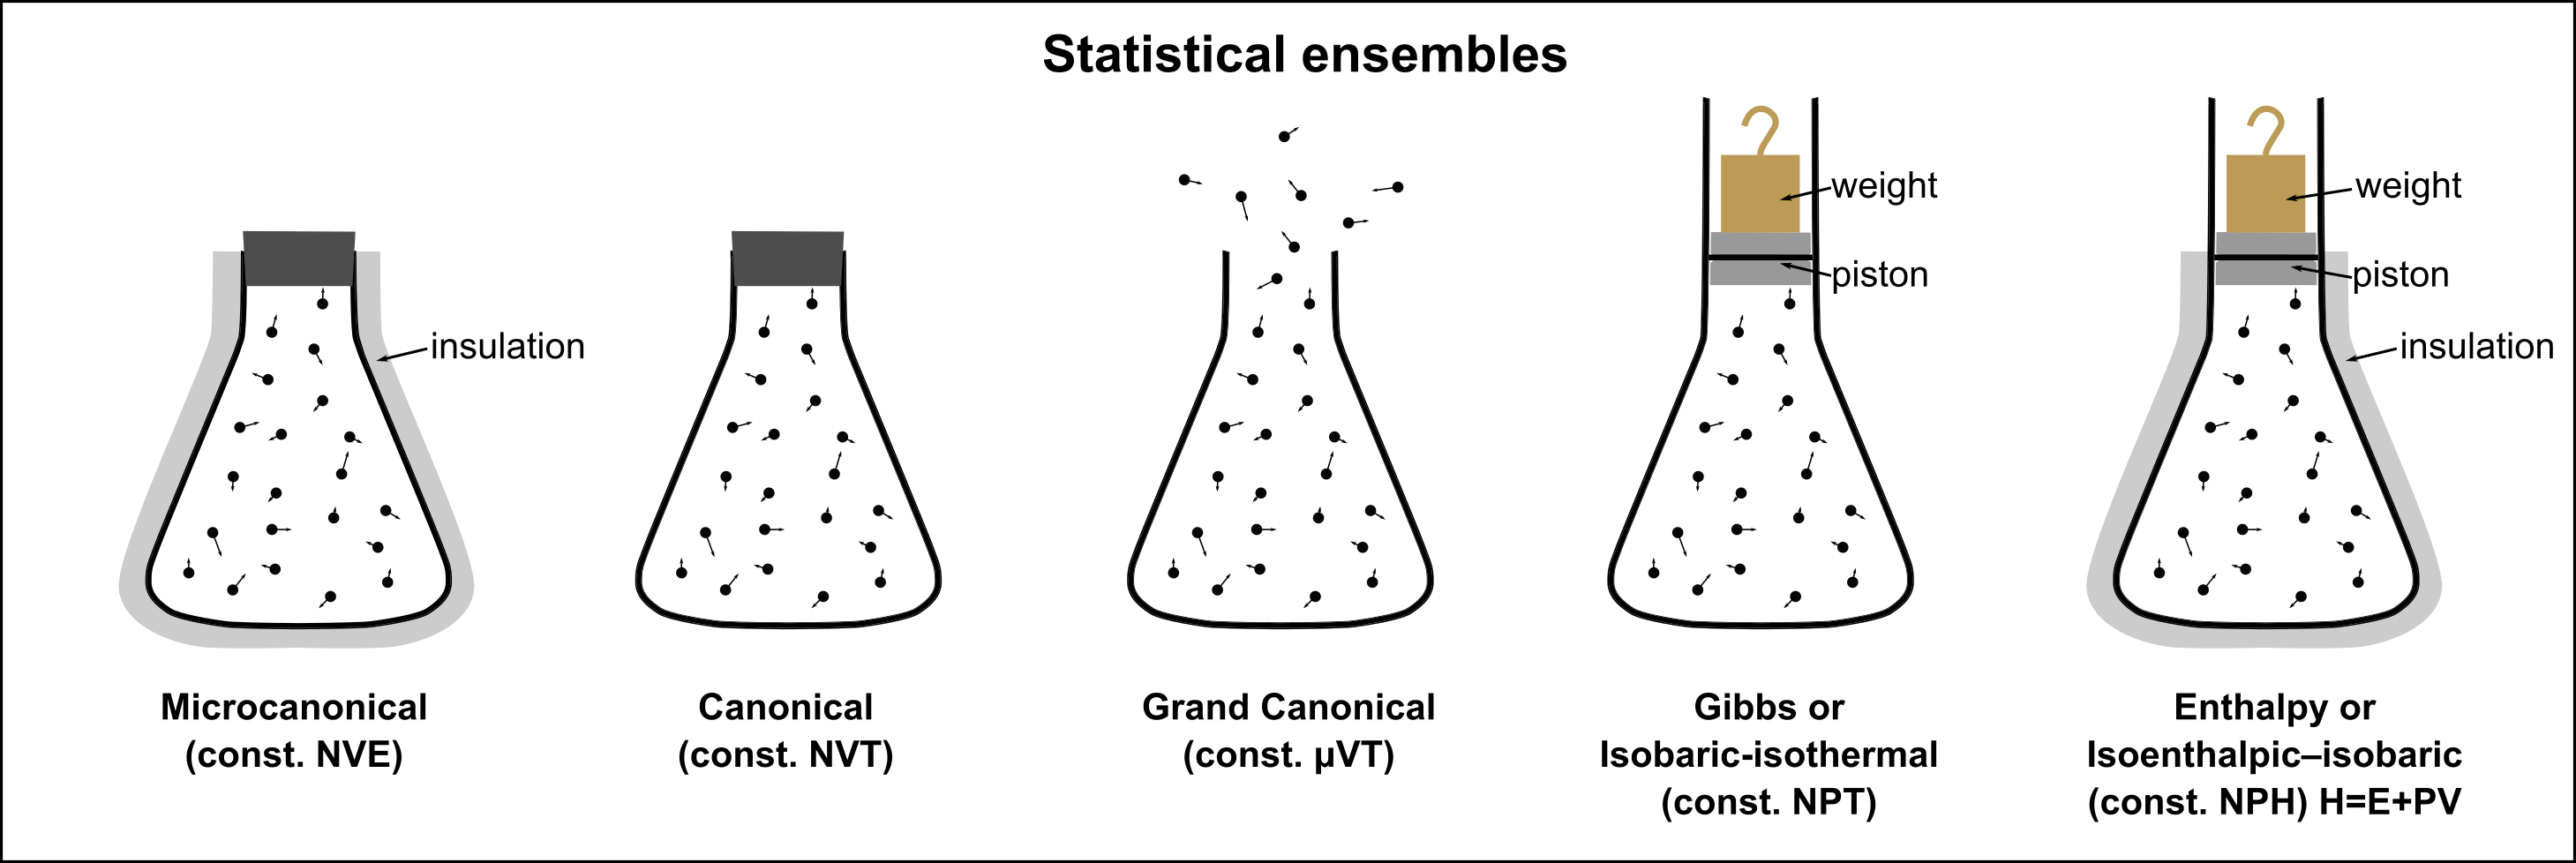
\includegraphics[height=1.60in,width=3.85in,viewport=0 0 1420 570,clip]{Figures/Statistical_Ensembles.png}
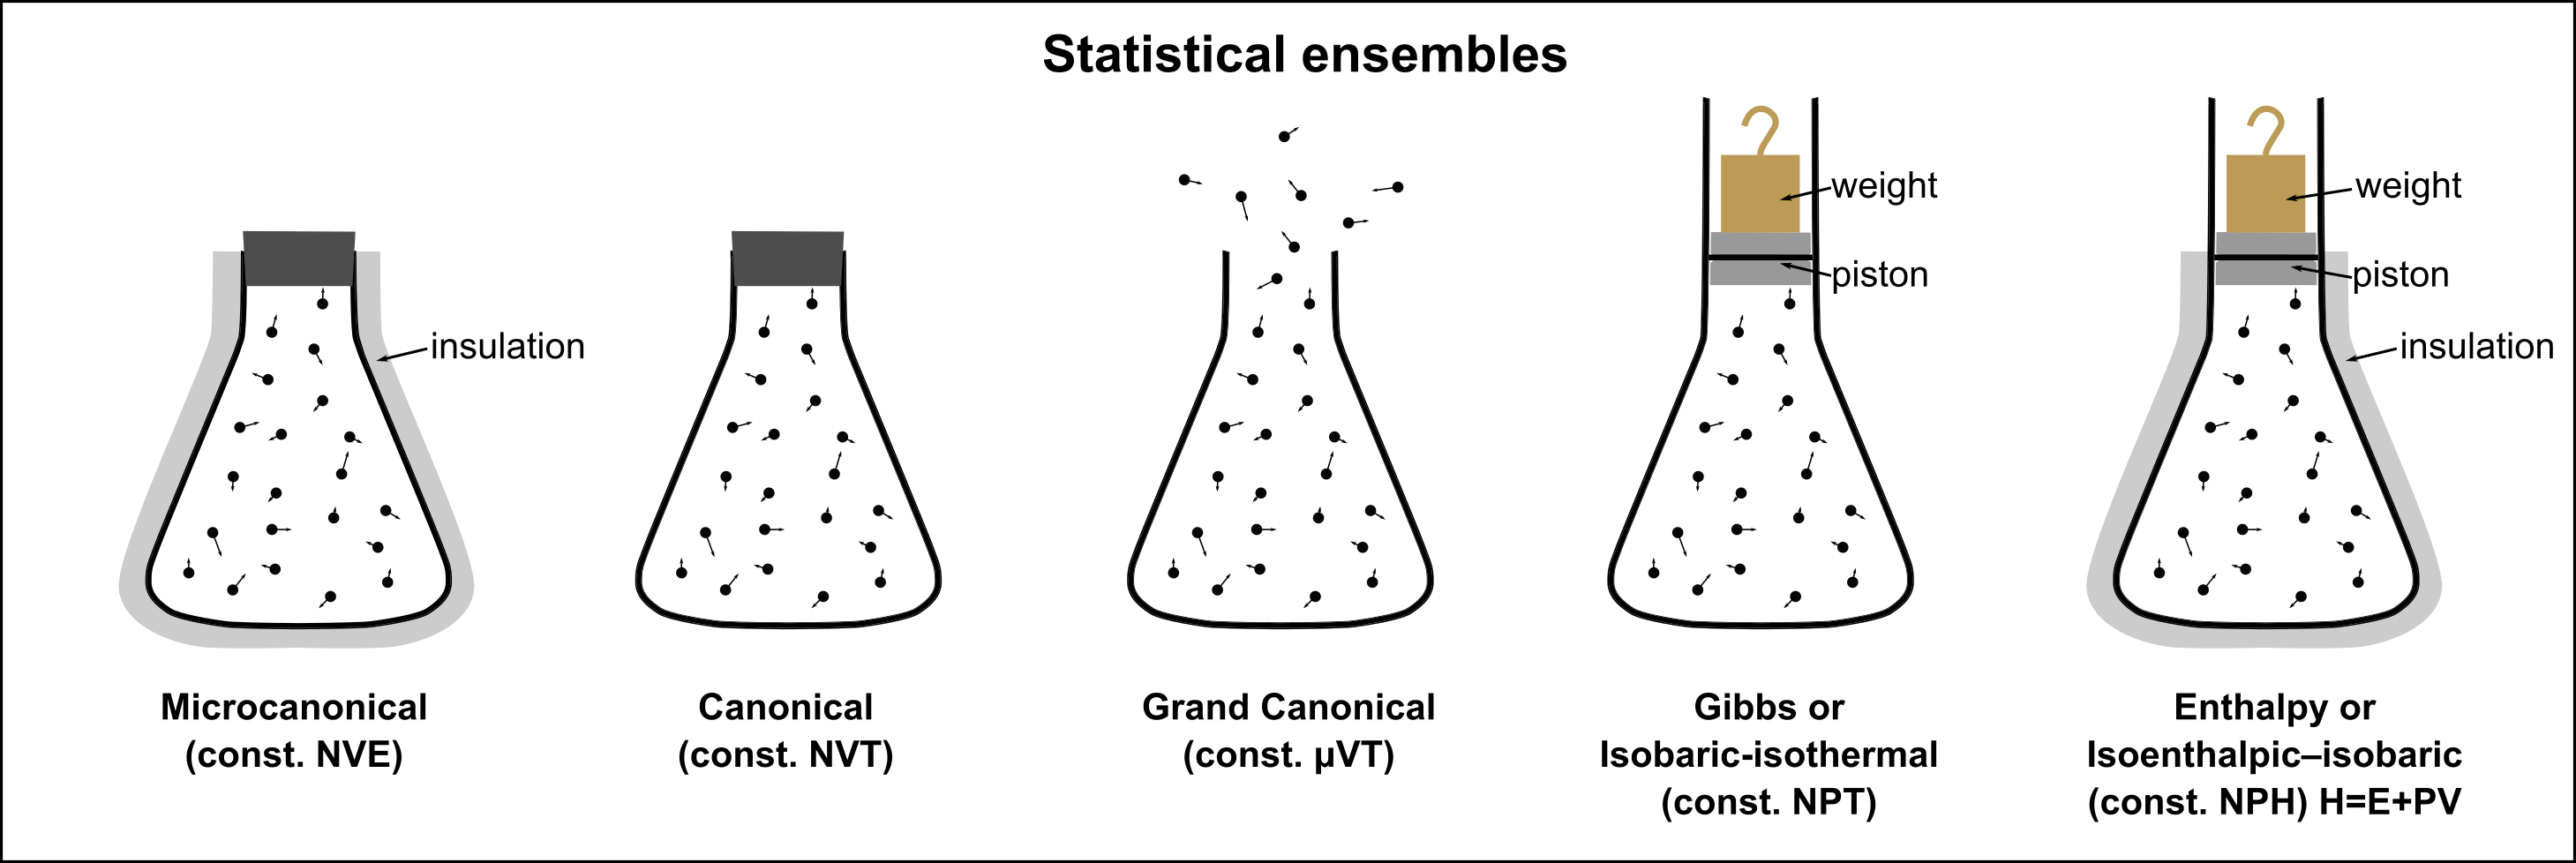
\includegraphics[height=1.20in,width=3.75in,viewport=0 0 1420 470,clip]{Figures/Statistical_Ensembles.png}
\caption{\tiny \textrm{The Statistical Ensembles.}}%(与文献\cite{EPJB33-47_2003}图1对比)
\label{Statistical_Ensembles}
\end{figure}
\vskip -15pt
\begin{itemize}
		{\fontsize{6.2pt}{1.2pt}\selectfont{
		\item 微正则系综\textrm{(Mircocanonical Ensemble)}%\footnote{\fontsize{4.5pt}{1.2pt}\selectfont{\textrm{canonical},汉译作``正则'',出自《楚辞\textperiodcentered 离骚》``皇揽揆余於初度兮,肇锡余以嘉名;~名余曰\textcolor{red}{正则}兮,字余曰灵均'',《楚辞章句》\upcite{Chucizhangju}:~``正,平也;~则,法也;~灵,神也;~均,调也。言正平可法则者,莫过于天;~养物均调者,莫神于地。高平曰原,故父伯庸名我为平以法天,字我为原以法地。言己上之能安君,下之能养民也。''意思是说``正则''、``灵均''隐喻着某种意义,即平正是天的象征,原均是地的象征。因此正则的含义是``\textcolor{blue}{符合天道}'',与\textrm{canonical}的意思\textrm{of, relating to, or forming a canon}意义一致。}}
			:~\textrm{NVE}皆为常数
		\item 正则系综\textrm{(Canonical Ensemble)}:~\textrm{NVT}皆为常数
		\item 巨正则系综\textrm{(Grandcanonical Ensemble)}:~\textrm{$\mu$VT}皆为常数,粒子数不固定
		\item 等压-等温系综\textrm{(Isobaric-Isothermal Ensemble)}:~\textrm{NPT}皆为常数
		\item 等焓-等压系综\textrm{(Isoenthalpic-Isobaric Ensemble)}:~\textrm{NPH}皆为常数
		\item 等张力-等温系综\textrm{(Isotension-Isothermal Ensemble)}:~容器形状可变 }}
\end{itemize}
}

\frame
{
	\frametitle{常用热力学量}
	\begin{itemize}
{\fontsize{7.8pt}{1.2pt}\selectfont{
		\item 动能 ~$E_{\mathrm{k}}=\bigg\langle\sum\limits_{i=1}^N\dfrac12m_iv_i^2\bigg\rangle$
		\item 势能 ~$E_{\mathrm{p}}=\bigg\langle\sum\limits_{i=1}^NE_{\mathrm{p}i}\bigg\rangle$
		\item 温度 ~$T=\dfrac1{\mathrm{d}Nk_{\mathrm{B}}}\bigg\langle\sum\limits_{i=1}^Nm_iv_i^2\bigg\rangle$ ~~~~ 其中$\mathrm{d}$是空间维度
		\item 压强 ~$p=\dfrac{k_{\mathrm{B}}TN}{V}+\dfrac1{\mathrm{d}V}\bigg\langle\sum\limits_{i<j}\vec f_{ij}\cdot\vec r_{ij}\bigg\rangle$
		\item 焓 ~$H=E+pV$ ~~~~ 相当于\textrm{NPT}下的有效总内能
		\item 熵 ~$S=k_{\mathrm{B}}\ln\Omega(N,V,E)$ ~~~~ $\Omega$是系统的总的微观状态数
		\item \textrm{Helmholtz}自由能:~\textcolor{blue}{\textrm{NVT}下的自由能}
			\begin{displaymath}
				F=E-TS=-k_{\mathrm{B}}T\ln{Q}
			\end{displaymath}
		\item \textrm{Gibbs}自由能:~\textcolor{blue}{\textrm{NPT}下的自由能}
			\begin{displaymath}
				G=F+pV=E-TS+pV
			\end{displaymath}
		\item 化学势 ~$\mu=\dfrac{\partial G}{\partial N}\bigg|_{T,p}=\dfrac{\partial F}{\partial N}\bigg|_{T,V}$}}
	\end{itemize}
}

\section{{\rm LAMMPS}软件基础}
\subsection{{\rm LAMMPS}软件}
\frame
{
	\frametitle{\textrm{LAMMPS}简介}
	\textcolor{blue}{\textrm{LAMMPS}}:\\
	\textrm{Large-scale Atomic/Molecular Massively Parallel Simulator}\\
	美国能源部的两个实验室和三个公司联合开发\\
	由\textrm{Sandia}国家实验室发布
	\begin{itemize}
			\setlength{\itemsep}{10pt}
		\item 固态、液态、气态的经典分子动力学模拟
		\item 易于扩展:~方便引入新的力场、原子类型和边界条件
		\item 开发语言:~\textrm{C++-MPI/FFT}
		\item 支持\textrm{GPU}计算,支持\textrm{OpenMP}
		\item 脚本可支持一个或多个模拟进程
	\end{itemize}
}

\frame
{
	\frametitle{模型\textrm{(atom\_style)}}
	\begin{itemize}
		\item 原子或简单分子
		\item 粗粒化粒子~(如有机高分子模型:~小球-弹簧模型)
		\item \textrm{United-atom}高分子或有机分子
		\item 全原子高分子:~有机分子、蛋白质、\textrm{DNA}
		\item 金属:~金属单质、合金
		\item 颗粒物质
		\item 粗粒化介观模型
		\item 有限尺度球和椭球粒子
		\item 有限尺度\textrm{line segment~(2d)}与三角\textrm{(3d)}粒子
		\item 偶极粒子
		\item 硬球粒子
		\item 上述模型的组合
	\end{itemize}
}

\frame[allowframebreaks]
{
	\frametitle{各类力场}
	\begin{itemize}
{\fontsize{9.5pt}{2.2pt}\selectfont{
		\item \textcolor{blue}{二体势}:~\textrm{Lennard-Jones, Buckingham, Morse, Born-Mayer-Huggins, Yukawa, soft, COMPASS,hydrogen bond, tabulated}
		\item \textcolor{blue}{带点二体势}:~\textrm{Coulomb}势,点电荷-电偶极矩作用
		\item \textcolor{blue}{多体势}:~\textrm{EAM, Finnis/Sinclair EAM, modified EAM~(MEAM), embedded ion method~(EIM), EDIP, ADP, Stillinger-Weber, Tersoff, REBO, AIREBO, ReaxFF, COMB}
		\item \textcolor{blue}{电子力场}:~\textrm{eFF, AWPMD}
		\item \textcolor{blue}{粗粒化势}:~\textrm{DPD, GayBerne, REsquared, colloidal, DLVO}
		\item \textcolor{blue}{介观势}:~\textrm{granular, Peridynamics, SPH}
		\item \textcolor{magenta}{Bond potentials}:~\textrm{harmonic, FENE, Morse, nonlinear, class 2, quartic (breakable)}
		\item \textcolor{magenta}{Angle potentials}:~\textrm{harmonic, CHARMM, cosine, cosine/squared, cosine/periodic, class 2~(COMPASS)}
		\item \textcolor{magenta}{Dihedral potentials}:~\textrm{harmonic, CHARMM, multi-harmonic, helix, class 2~(COMPASS), OPLS}
		\item \textcolor{magenta}{Improper potentials}:~\textrm{harmonic, cvff, umbrella, class 2~(COMPASS)}
		\item \textcolor{purple}{高分子势}:~\textrm{all-atom, united-atom,bead-spring, breakable}
		\item \textcolor{purple}{水分子势}:~\textrm{TIP3P, TIP4P, SPC}
		\item \textcolor{purple}{隐含溶液势}:~\textrm{hydrodynamic lubrication, Debye}
		\item \textcolor{blue}{\textrm{KIM archive of potentials}}
		\item \textcolor{purple}{长程势}:~\textrm{Ewald, Wolf, PPPM~(similar to particle-mesh Ewald), Ewald/N for long-range Lennard-Jones}
		\item 与常用力场\textrm{CHARMM, AMBER, DREIDING, OPLS, GROMACS, COMPASS}格式兼容}}
	\end{itemize}
}

\frame
{
	\frametitle{初始构型}
	\begin{itemize}
		\item \textcolor{blue}{read\_data}:\\
			从构型文件中读入原子坐标
		\item \textcolor{blue}{lattice}:\\
			确定空间格子类型
		\item \textcolor{blue}{create\_atoms}:\\
			在格点上摆放原子
		\item \textcolor{blue}{delete\_atoms}:\\
			在给定构型上删除成组原子
		\item \textcolor{blue}{displace\_atoms}:\\
			移动已有原子位置
		\item \textcolor{blue}{replicate}:\\
			复制已有构型,可多次复制
	\end{itemize}
}

\frame
{
	\frametitle{系综与约束\textrm{(fix)}条件}
	\begin{itemize}
		\item 空间二维或三维的系统
		\item 正交或非正交晶系(含三斜晶系)
		\item \textrm{NVE, NVT, NPT, NPH, Parinello/Rahman}积分器
		\item 针对原子组群可以指定不同的热耦
		\item 通过\textrm{Nose/Hoover}或者\textrm{Berendsen}压耦控制压强
		\item 模拟容器的变形(拉伸或剪切)
		\item 谐振函数约束的力(回复力)
		\item 刚体约束,\textrm{SHAKE}算法固定键长和键角
		\item 化学键的断裂、形成与交换
		\item 各类边界条件
		\item 非平衡态分子动力学模拟
	\end{itemize}
}

\frame
{
	\frametitle{积分算法}
	\begin{itemize}
		\item \textcolor{blue}{run}:\\
			运行\textrm{run}命令,执行(积分)模拟过程
		\item \textcolor{blue}{run\_style}:\\
			配套\textrm{run}命令使用,不一定需要
		\item \textrm{velocity-Verlet}积分器
		\item \textrm{Brown}运动积分
		\item 刚体积分
		\item \textcolor{blue}{minimize}:\\
			共轭梯度或最陡下降法进行能量优化
		\item \textrm{rRESPA}多等级时间步长
		\item \textcolor{blue}{return}:\\
			\textrm{return}命令,重新运行模拟过程
	\end{itemize}
}

\frame
{
	\frametitle{数据输出}
	\begin{itemize}
		\item \textcolor{green}{log}:\\
			\textrm{log}文件输出热力学信息\\
文本文件输出原子坐标、速度等基本信息
\item \textcolor{green}{restart}:\\
	二进制重启文件
\item 并行输出的文件流
\item 热力学量~(能量、压力等等状态函数)
\item 用户定义的计算
\item 热力学量的时间平均
\item \textrm{XYZ, XTC, DCD, CFG}和自定义格式的原子构型
	\end{itemize}
}

\frame
{
	\frametitle{\textrm{LAMMPS}的文件}
	\begin{itemize}
			\setlength{\itemsep}{10pt}
			\item \textcolor{blue}{\textrm{Input File}}:~文本文件\\由\textrm{LAMMPS}完成模拟所执行的全部命令
			\item \textcolor{blue}{\textrm{Log File}}:~文本文件\\模拟过程中的热力学数据的输出
			\item \textcolor{blue}{\textrm{Dump File}}:~原子的受力,也被称为原子性质快照\textrm{(sanapshot of atom properties)}
			\item \textcolor{blue}{\textrm{Restart File}}:~二进制文件\textrm{(binary checkpoint file)}\\包含重启模拟所需的全部数据
			\item \textcolor{blue}{\textrm{Data File}}:~文本文件\\包含用于启动计算或重启计算的数据 
	\end{itemize}
}

\frame
{
	\frametitle{多重交换模型}
	\begin{itemize}
			\setlength{\itemsep}{10pt}
		\item \textrm{Nudged elastic band}:\\
			寻找局域最优的反应路径
		\item \textrm{Parallel replica dynamics}:\\
			通过多个短模拟估算单个跃迁事件所需的时间
		\item \textrm{Temperature accelerated dynamics}:\\
			通过高温模拟以加速动力学过程
		\item \textrm{Parallel tempering (replica exchange)}:\\
			同时执行不同问题的模拟,通过高温的模拟辅助低温模型提高采样效率
	\end{itemize}
}

\frame
{
	\frametitle{前后处理与可视化工具}
	\textrm{\textcolor{blue}{LAMMPS}}提供了各种串行的前后处理的工具软件
\vskip 15pt
	\textcolor{brown}{\textrm{Pizzaa.py}}软件包:\\\
	包括创建输入文件、分析、绘制数据图和计算结果可视化等功能
\vskip 15pt
分子构型绘图软件 
	\begin{itemize}
			\setlength{\itemsep}{8pt}
		\item \textcolor{red}{xmakemol}:\\
			简单软件,方法绘制矢量图~(只能用\textrm{XYZ}格式的输入文件)
		\item \textcolor{red}{VMD}:\\
			\textrm{UIUC}的\textrm{Klaus Schulten}组开发,与\textrm{\textcolor{blue}{NAMD}}配套使用\\
			\textrm{VMD}功能强大,有自己的\textrm{script}语言,能完成简单的\textrm{MD}模拟辅助功能,特别适合针对生物体系的作图
	\end{itemize}
}

\frame
{
	\frametitle{\textrm{LAMMPS}的特殊功能}
	\begin{itemize}
			\setlength{\itemsep}{5pt}
		\item 随机转动动力学
		\item 实时可视化和交互分子动力学模拟
		\item 有限元方法实现的原子与连续模型的耦合
		\item 通过\textrm{POEMS}库实现耦合刚体的积分
		\item 巨正则系综\textrm{$\mu$VT}的\textrm{Monte-Carlo}模拟插入和删除粒子
		\item 低密度流体的\textrm{Monte-Carlo}直接模拟
		\item \textcolor{blue}{Peridynamics}:\\
			应用近场动力学方法完成介观尺度粒子模拟
		\item \textrm{Targeted MD}与\textrm{Steered MD}
	\end{itemize}
}

\frame
{
	\frametitle{\textrm{LAMMPS}不具备的功能}
	\begin{itemize}
			\setlength{\itemsep}{10pt}
			\item %\textrm{\textcolor{blue}{LAMMPS}}
				没有提供图形界面用以执行模拟命令
		\item 没有自带的分子模型建模工具
		\item 没有默认设定通用的力场参数
		\item 无法对复杂的模拟结果进行深入分析
		\item 没有自带的模拟结果可视化工具\\
			必须借助诸如\textcolor{red}{xmakemol}或\textcolor{red}{VMD}等外部软件
		\item 无法对输出数据直接作图
	\end{itemize}
}

\subsection{{\rm LAMMPS}的输入文件格式}
\frame[allowframebreaks]
{
	\frametitle{构型文件}
	\begin{itemize}
		\item $\ast\ast\ast\ast\ast\ast\ast\ast$ ~~~~~~~~~~~~~~~~~~  标题
			\vskip 8pt
		\item \textrm{XXX} \textcolor{blue}{\textrm{atoms}} ~~~~~~~~~~~~~~~~~~ 体系的总原子数
		\item \textrm{XXX} \textcolor{blue}{\textrm{bonds}} ~~~~~~~~~~~~~~~~~~ 体系的总键数
		\item \textrm{XXX} \textcolor{blue}{\textrm{angles}} ~~~~~~~~~~~~~~~~~~ 体系的总角度数
		\item \textrm{XXX} \textcolor{blue}{\textrm{dihedrals}} ~~~~~~~~~~~~~~ 体系的总二面角数
		\item \textrm{XXX} \textcolor{blue}{\textrm{impropers}} ~~~~~~~~~~~~~ 体系的总\textrm{improper dihedral}数
\vskip 8pt
		\item \textrm{XXX} \textcolor{blue}{\textrm{atom types}} ~~~~~~~~~~~~ 体系的原子类型数
		\item \textrm{XXX} \textcolor{blue}{\textrm{bond types}} ~~~~~~~~~~~~ 体系的化学键类型数
		\item \textrm{XXX} \textcolor{blue}{\textrm{angle types}} ~~~~~~~~~~~~ 体系的键角类型数
		\item \textrm{XXX} \textcolor{blue}{\textrm{dihedral types}} ~~~~~~~~ 体系的二面角类型数
		\item \textrm{XXX} \textcolor{blue}{\textrm{improper types}} ~~~~~~~~ 体系的\textrm{improper dihedral}类型数
			\vskip 8pt
		\item \textrm{XXX ~ XXX} \textcolor{blue}{\textrm{~ xlo ~ xhi}} ~~~~~ 模拟盒子在$x$方向的范围
		\item \textrm{XXX ~ XXX} \textcolor{blue}{\textrm{~ ylo ~ yhi}} ~~~~~ 模拟盒子在$y$方向的范围
		\item \textrm{XXX ~ XXX} \textcolor{blue}{\textrm{~ zlo ~ zhi}} ~~~~~ 模拟盒子在$z$方向的范围
			\vskip 8pt
		\item \textcolor{blue}{\textrm{Masses}}
			\vskip 2pt
		\{\textrm{atom-type ~ mass}\}
			\vskip 8pt
		\item \textcolor{blue}{\textrm{Pair Coeffs}}
			\vskip 2pt
		\{\textrm{pair-type ~ p1 ~ p2 ~ p3 ~ p4}\}
			\vskip 8pt
		\item \textcolor{blue}{\textrm{Bond Coeffs}}
			\vskip 2pt
		\{\textrm{bond-type ~ p1 ~ p2}\}
			\vskip 8pt
		\item \textcolor{blue}{\textrm{Angle Coeffs}}
			\vskip 2pt
		\{\textrm{angle-type ~ p1 ~ p2}\}
			\vskip 8pt
		\item \textcolor{blue}{\textrm{Dihedral Coeffs}}
			\vskip 2pt
		\{\textrm{dihedral-type ~ p1 ~ p2 ~p3}\}
			\vskip 8pt
		\item \textcolor{blue}{\textrm{Improper Coeffs}}
			\vskip 2pt
		\{\textrm{improper-type ~ p1 ~ p2 ~p3}\}
			\vskip 8pt
		\item \textcolor{blue}{\textrm{Atoms}}
			\vskip 2pt
	 	\{\textrm{atom-ID ~ molecule-ID ~ atom-type ~ q ~ x ~ y ~ z}\}
			\vskip 8pt
		\item \textcolor{blue}{\textrm{Velocities}}
			\vskip 2pt
		\{\textrm{atom-ID ~ vx ~ vy ~ vz}\}
			\vskip 8pt
		\item \textcolor{blue}{\textrm{Bonds}}
			\vskip 2pt
		\{\textrm{bond-ID ~ bond-type ~ atom-ID1 ~ atom-ID2}\}
			\vskip 8pt
		\item \textcolor{blue}{\textrm{Angles}}
			\vskip 2pt
		\{\textrm{angle-ID ~ angle-type ~ atom-ID1 ~ atom-ID2 ~ atom-ID3}\}
			\vskip 8pt
		\item \textcolor{blue}{\textrm{Dihedrals}}
			\vskip 2pt
		\{\textrm{dihedral-ID ~ dihedral-type ~ atom-ID1 ~ atom-ID2 ~ atom-ID3 ~ atom-ID4}\}
			\vskip 8pt
		\item \textcolor{blue}{\textrm{Impropers}}
			\vskip 2pt
		\{\textrm{improper-ID ~ improper-type ~ atom-ID1 ~ atom-ID2 ~ atom-ID3 ~ atom-ID4}\}
	\end{itemize}
}

\frame[allowframebreaks]
{
	\frametitle{参数文件}
	\begin{itemize}
		\item \#~$\ast\ast\ast\ast\ast\ast\ast\ast$ ~~~~~~~~~~~~ 标题
			\vskip 4pt
		\item \textcolor{blue}{units} ~ $\ast\ast\ast$ ~~~~~~~~~~~~~~~~ 能量单位
		\item \textcolor{blue}{atom\_style} ~ $\ast\ast\ast$ ~~~~~~~~ 原子构型格式
		\item \textcolor{blue}{boundary} ~ $\ast\ast\ast$ ~~~~~~~~~~~ 周期边界条件
		\item \textcolor{blue}{pair\_style} ~ $\ast\ast\ast$ ~~~~~~~~~~ 非成键相互作用的函数形式
		\item \textcolor{blue}{pair\_modify} ~ $\ast\ast\ast$ ~~~~~~~ 修改非成键相互作用的函数形式
		\item \textcolor{blue}{bond\_style} ~ $\ast\ast\ast$ ~~~~~~~~ 化学键类型
		\item \textcolor{blue}{angle\_style} ~ $\ast\ast\ast$ ~~~~~~~~ 键角类型
		\item \textcolor{blue}{dihedral\_modify} ~ $\ast\ast\ast$ ~~ 二面角类型
		\item \textcolor{blue}{improper\_style} ~ $\ast\ast\ast$ ~~~~ \textrm{improper dihedral}类型
		\item \textcolor{blue}{kspace\_style} ~ $\ast\ast\ast$ ~~~~~~ 长程力算法
			\vskip 4pt
		\item \textcolor{blue}{read\_data} ~ $\ast\ast\ast$ ~~~~~~~~~ 指定读入数据文件名
		\item \textcolor{blue}{neighbor} ~ $\ast\ast\ast$ ~~~~~~~~~~~ 设定\textrm{neighbor list}参数
		\item \textcolor{blue}{neigh\_modify} ~ $\ast\ast\ast$ ~~~~~ 原子类型格式
			\vskip 4pt
		\item \textcolor{blue}{timestep} ~ $\ast\ast\ast$ ~~~~~~~~~~~ 时间步长;~单位取决于\textrm{units}的设置
			\vskip 4pt
		\item \textcolor{blue}{thermo\_style} ~ $\ast\ast\ast$ ~~~~~ 输出文件的数据内容
		\item \textcolor{blue}{thermo} ~ \textrm{XXX} ~~~~~~~~~~~~ 输出数据间隔
			\vskip 4pt
		\item \textcolor{blue}{fix} ~ $\ast\ast\ast$ ~~~~~~~~~~~~~~~~~~~ 设定模拟系综及参数等
			\vskip 4pt
		\item \textcolor{blue}{dump} ~ $\ast\ast\ast$ ~~~~~~~~~~~~~~~ 设定输出构型文件名及参数
			\vskip 4pt
		\item \textcolor{blue}{run} ~ \textrm{XXX} ~~~~~~~~~~~~~~~~~ 输运行的总步长
			\vskip 4pt
		\item \textcolor{blue}{write restart} ~ $\ast\ast\ast$ ~~~~~~~ 断点保存的文件名
	\end{itemize}
}

\subsection{{\textrm LAMMPS}命令}
\frame[allowframebreaks]
{
	\frametitle{\textrm{LAMMPS}命令的特点和分类}
	\textrm{LAMMPS}命令的特点
	\begin{itemize}
		\item \textrm{LAMMPS}采用逐行解释执行命令形式
		\item \textcolor{blue}{命令}都用\textcolor{red}{小写字母}表示,\textcolor{blue}{文件名}和\textcolor{blue}{变量}都用\textcolor{red}{大写字母}表示
		\item 特殊字符的含义:~\textcolor{purple}{\&}:~续行;~\textcolor{purple}{\#}:~注释;~\textcolor{purple}{\$}:~变量
	\end{itemize}
	\textrm{LAMMPS}命令的分类
	\begin{itemize}
			\setlength{\itemsep}{10pt}
		\item 初始化命令:\\
			\textcolor{blue}{atom\_modify},\textcolor{blue}{atom\_style},\textcolor{blue}{boundary},\textcolor{blue}{dimension},\textcolor{blue}{newton},\\\textcolor{blue}{processors},\textcolor{blue}{units}
		\item 初始构型命令:\\
			\textcolor{blue}{create\_atoms},\textcolor{blue}{create\_box},\textcolor{blue}{lattice},\textcolor{blue}{read\_data},\textcolor{blue}{read\_dump},\\\textcolor{blue}{read\_restart},\textcolor{blue}{region},\textcolor{blue}{replicate}
		\item 力场命令:\\
			\textcolor{blue}{angle\_coeff},\textcolor{blue}{angle\_style},\textcolor{blue}{bond\_coeff},\textcolor{blue}{bond\_style},\textcolor{blue}{dielectric},\\
			\textcolor{blue}{dihedral\_coeff},\textcolor{blue}{dihedral\_style},\textcolor{blue}{improper\_coeff},\textcolor{blue}{improper\_style},\\
			\textcolor{blue}{kspace\_modify},\textcolor{blue}{kspace\_style},\textcolor{blue}{pair\_coeff},\textcolor{blue}{pair\_style},\textcolor{blue}{pair\_write},\\
			\textcolor{blue}{special\_bonds}
		\item 设置命令:\\
			\textcolor{blue}{communicate},\textcolor{blue}{group},\textcolor{blue}{mass},\textcolor{blue}{min\_modify},\textcolor{blue}{min\_style},\textcolor{blue}{neigh\_modify},\\\textcolor{blue}{neighbor},\textcolor{blue}{rest\_timestep},\textcolor{blue}{run\_style},\textcolor{blue}{set},\textcolor{blue}{timestep},\textcolor{blue}{velocity}
		\item \textrm{Fix}命令:\\
			\textcolor{blue}{fix},\textcolor{blue}{fix\_modify},\textcolor{blue}{unfix}
		\item \textrm{Compute}命令:\\
			\textcolor{blue}{compute},\textcolor{blue}{compute\_modify},\textcolor{blue}{uncompute}
		\item 设置命令:\\
			\textcolor{blue}{dump},\textcolor{blue}{dump\_image},\textcolor{blue}{dump\_modify},\textcolor{blue}{restart},\textcolor{blue}{thermo},\textcolor{blue}{thermo\_modify},\\\textcolor{blue}{thermo\_style},\textcolor{blue}{undump},\textcolor{blue}{write\_restart}
		\item 运行命令:\\
			\textcolor{blue}{delete\_atoms},\textcolor{blue}{delete\_bonds},\textcolor{blue}{displace\_atoms},\textcolor{blue}{change\_box},\textcolor{blue}{minimize},\\\textcolor{blue}{neb\_prd},\textcolor{blue}{return},\textcolor{blue}{run},\textcolor{blue}{temper}
		\item 其它命令:\\
			\textcolor{blue}{clear},\textcolor{blue}{echo},\textcolor{blue}{if},\textcolor{blue}{include},\textcolor{blue}{jump},\textcolor{blue}{label},\textcolor{blue}{log},\textcolor{blue}{next},\textcolor{blue}{print},\textcolor{blue}{shell},\textcolor{blue}{variable}
	\end{itemize}
}

\frame
{
	\frametitle{}
	\begin{itemize}
		\item \textcolor{magenta}{Fix}命令:~设置模拟系综、算法、条件、参数等
	\end{itemize}
\begin{figure}[h!]
\centering
\vspace*{-0.1in}
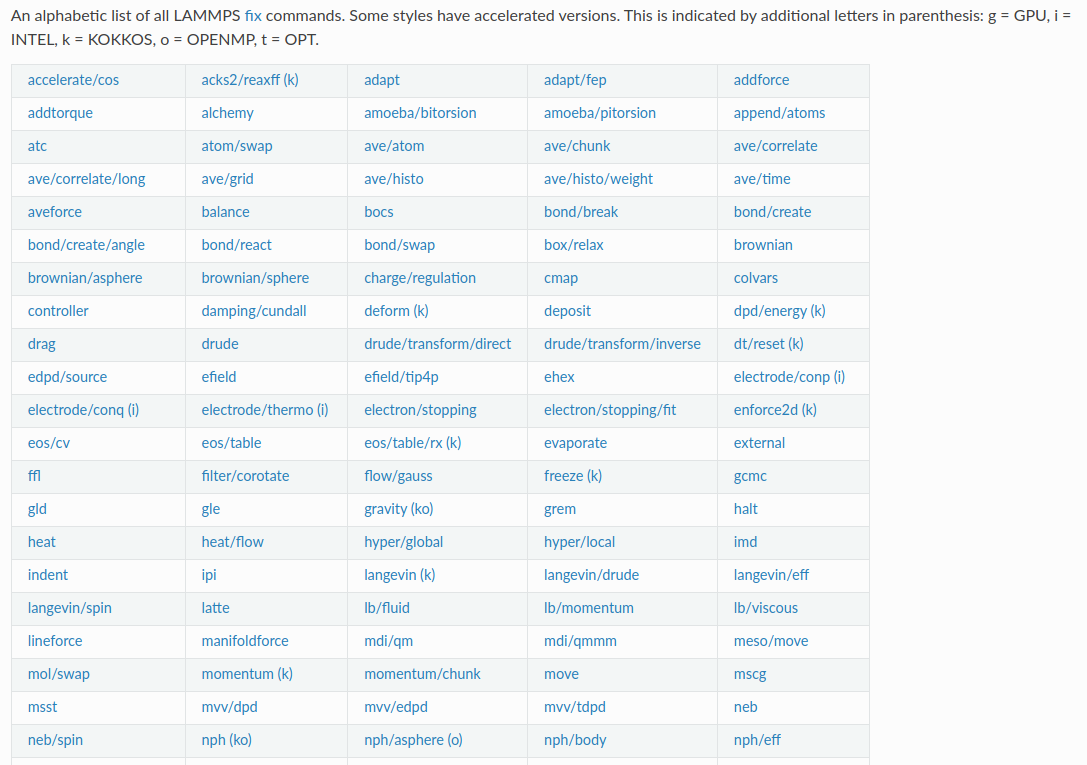
\includegraphics[height=2.4in,width=3.4in,viewport=0 0 1100 760,clip]{Figures/LAMMPS-fix_command.png}
%\caption{\fontsize{5.5pt}{2.2pt}\selectfont{\textrm{The structure factor of argon calculating from a radial distribution function.}}}%(与文献\cite{EPJB33-47_2003}图1对比)
\label{LAMMPS-Fix}
\end{figure}
}

\frame
{
	\frametitle{}
	\begin{itemize}
		\item \textcolor{magenta}{Compute}命令:~设置实时运行中完成的数据处理运算
	\end{itemize}
\begin{figure}[h!]
\centering
\vspace*{-0.1in}
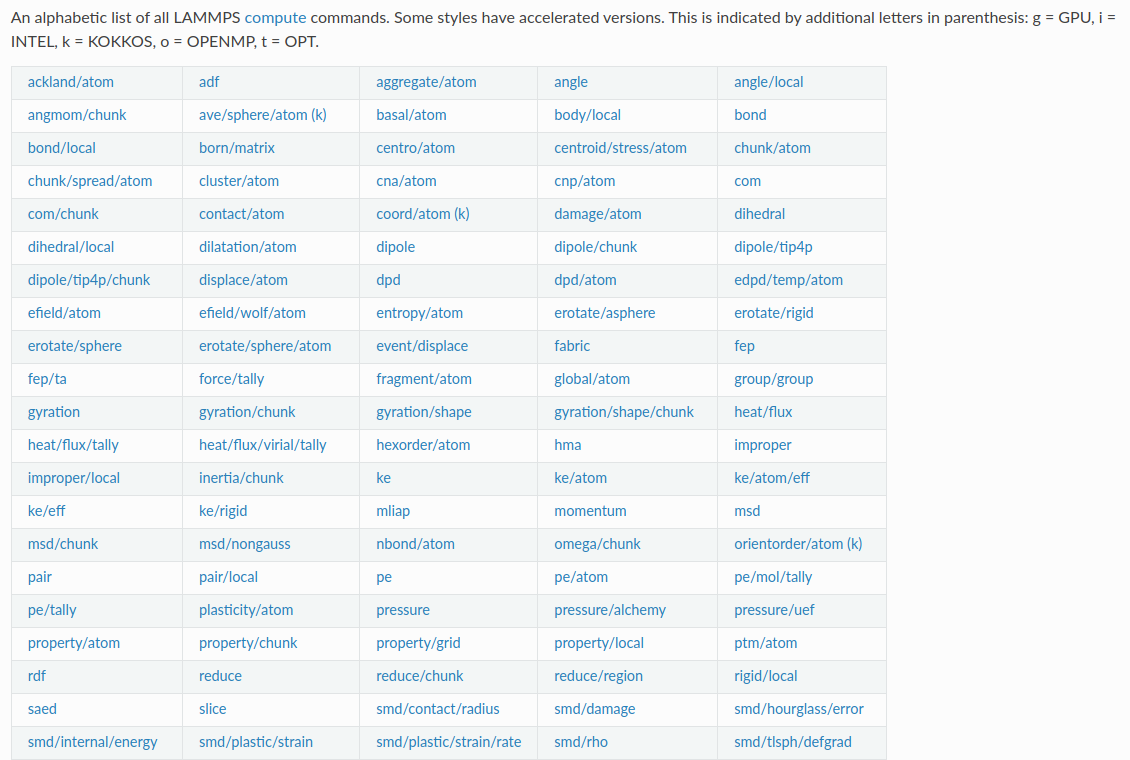
\includegraphics[height=2.4in,width=3.4in,viewport=0 0 1150 760,clip]{Figures/LAMMPS-compute_command.png}
%\caption{\fontsize{5.5pt}{2.2pt}\selectfont{\textrm{The structure factor of argon calculating from a radial distribution function.}}}%(与文献\cite{EPJB33-47_2003}图1对比)
\label{LAMMPS-Compute}
\end{figure}
}

\frame
{
	\frametitle{}
	\begin{itemize}
		\item \textcolor{magenta}{Pair\_style}:~非成键相互作用的设置
	\end{itemize}
\begin{figure}[h!]
\centering
\vspace*{-0.1in}
\includegraphics[height=2.2in,width=3.4in,viewport=0 0 1100 760,clip]{Figures/LAMMPS-Pair_style-command.png}
%\caption{\fontsize{5.5pt}{2.2pt}\selectfont{\textrm{The structure factor of argon calculating from a radial distribution function.}}}%(与文献\cite{EPJB33-47_2003}图1对比)
\label{LAMMPS-Pair_style}
\end{figure}
}

\frame
{
	\frametitle{}
	\begin{itemize}
		\item \textcolor{magenta}{Bond\_style}:~化学键的设置
\begin{figure}[h!]
\centering
\vspace*{-0.1in}
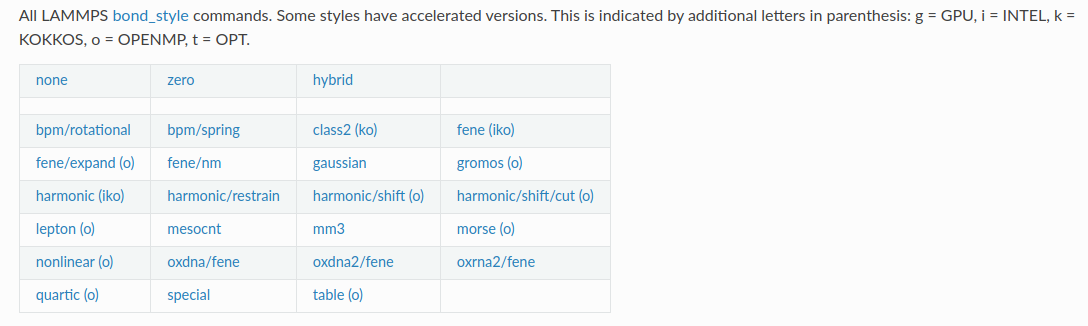
\includegraphics[height=1.0in,width=3.4in,viewport=0 0 1100 350,clip]{Figures/LAMMPS-bond_style-command.png}
%\caption{\fontsize{5.5pt}{2.2pt}\selectfont{\textrm{The structure factor of argon calculating from a radial distribution function.}}}%(与文献\cite{EPJB33-47_2003}图1对比)
\label{LAMMPS-bond_style}
\end{figure}
		\item \textcolor{magenta}{Angle\_style}:~键角的设置
\begin{figure}[h!]
\centering
\vspace*{-0.1in}
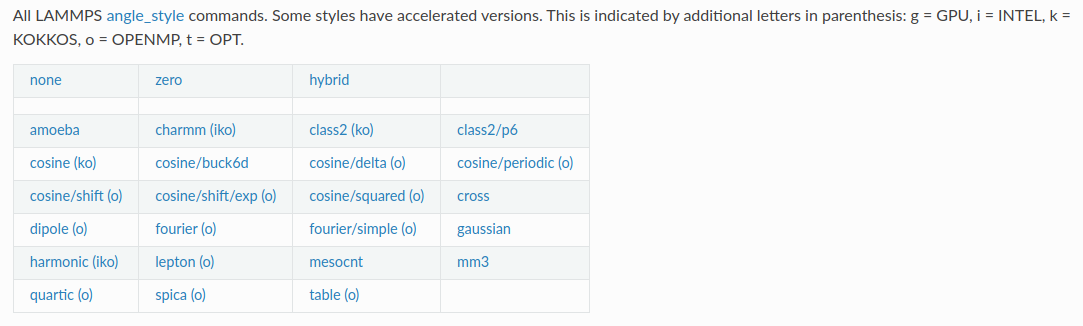
\includegraphics[height=1.0in,width=3.4in,viewport=0 0 1100 350,clip]{Figures/LAMMPS-angle_style-command.png}
%\caption{\fontsize{5.5pt}{2.2pt}\selectfont{\textrm{The structure factor of argon calculating from a radial distribution function.}}}%(与文献\cite{EPJB33-47_2003}图1对比)
\label{LAMMPS-angle_style}
\end{figure}
	\end{itemize}
}

\frame
{
	\frametitle{}
	\begin{itemize}
		\item \textcolor{magenta}{Dihedral\_style}:~二面角的设置
\begin{figure}[h!]
\centering
\vspace*{-0.10in}
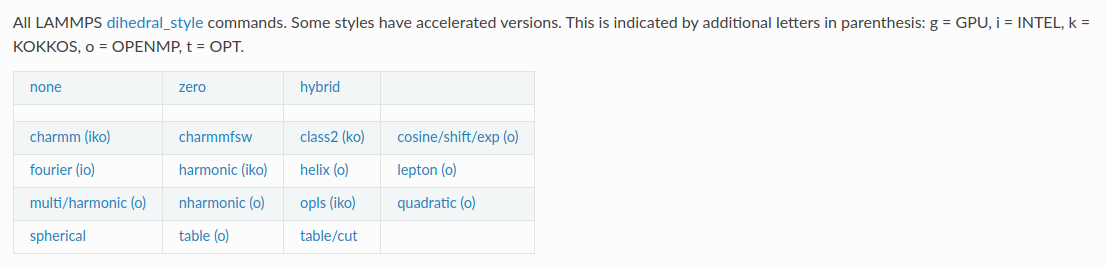
\includegraphics[height=0.8in,width=3.4in,viewport=0 0 1100 290,clip]{Figures/LAMMPS-dihedral_style-command.png}
%\caption{\fontsize{5.5pt}{2.2pt}\selectfont{\textrm{The structure factor of argon calculating from a radial distribution function.}}}%(与文献\cite{EPJB33-47_2003}图1对比)
\label{LAMMPS-dihedral_style}
\end{figure}
		\item \textcolor{magenta}{Improper\_style}:~\textrm{Improper dihedral}的设置
\begin{figure}[h!]
\centering
\vspace*{-0.10in}
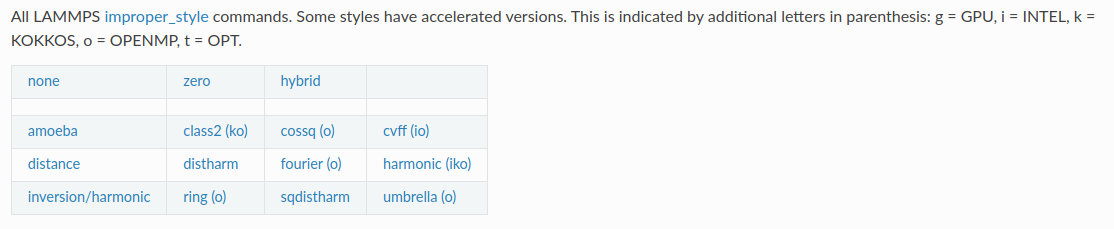
\includegraphics[height=0.8in,width=3.4in,viewport=0 0 1100 280,clip]{Figures/LAMMPS-improper_dihedral-command.png}
%\caption{\fontsize{5.5pt}{2.2pt}\selectfont{\textrm{The structure factor of argon calculating from a radial distribution function.}}}%(与文献\cite{EPJB33-47_2003}图1对比)
\label{LAMMPS-improper_dihedral}
\end{figure}
	\end{itemize}
}

\frame
{
	\frametitle{}
	\begin{itemize}
		\item \textcolor{magenta}{Kspace\_style}长程力算法命令
\begin{figure}[h!]
\centering
\vspace*{-0.10in}
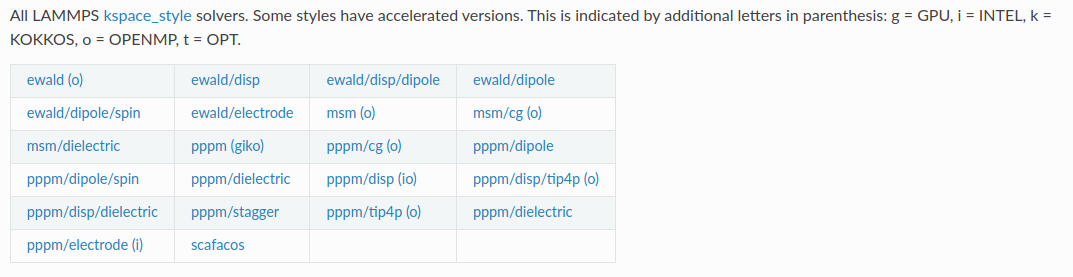
\includegraphics[height=0.9in,width=3.4in,viewport=0 0 1100 300,clip]{Figures/LAMMPS-kspace_style-command.png}
%\caption{\fontsize{5.5pt}{2.2pt}\selectfont{\textrm{The structure factor of argon calculating from a radial distribution function.}}}%(与文献\cite{EPJB33-47_2003}图1对比)
\label{LAMMPS-kspace_style}
\end{figure}
		\item 另外还有很多扩展命令:~对应于相应的扩展软件包
	\end{itemize}
}
%------------------------------------------------------------------------Reference----------------------------------------------------------------------------------------------
		\frame[allowframebreaks]
{
\frametitle{主要参考文献}
\begin{thebibliography}{99}
{\tiny
	\bibitem{CMS6-15_1996}\textrm{G. Kresse and J. Furthm\"uller \textit{Comput. Mat. Sci.}, \textbf{6} (1996), 15}
	\bibitem{PRB54-11169_1996}\textrm{G. Kresse and J. Furthm\"uller \textit{Phys. Rev.} B, \textbf{54} (1996), 11169}
	\bibitem{PRL55-2471_1985}\textrm{R. Car and M. Parrinello \textit{Phys. Rev.} Lett., \textbf{55} (1985), 2471}
	\bibitem{JCP27-1208_1957}\textrm{B.J. Alder, T.E. Wainwright. \textit{J. Chem. Phys.} \textbf{27} (1957), 1208}
	\bibitem{PRB47-10142_1993}\textrm{K. Laasonen and A. Pasquarello and R. Car and C. Lee and D. Vanderbilt \textit{Phys. Rev.} B, \textbf{47} (1993), 10142}
	\bibitem{Chucizhangju}[东汉]王逸~撰. \textit{楚辞章句}\:上海古籍出版社, 上海, 2017
	\bibitem{Elect_Stru}\textrm{Richard. M. Martin. \textit{Electronic Structure: Basic Theory and Practical Methods} (Cambridge University Press, Cambridge, England, 2004)}
	\bibitem{Comp_Phys}\textrm{J. M. Thijssen. \textit{Computational Physics (2nd Edition)} (Cambridge University Press, Cambridge, England, 2007)}
        \bibitem{Singh}\textrm{D. J. Singh. \textit{Plane Wave, PseudoPotential and the LAPW method} (Kluwer Academic, Boston,USA, 1994)}					%
	\bibitem{Lammps_turtorial}{\fzsong 王延颋}, \textrm{LAMMPS}教程~中科院超算中心培训, 北京, \textrm{2012}
}
\end{thebibliography}
%\nocite*{}
}
%-----------------------------------------------------------------------------------------------------------------------------------------------------------------------%
